\documentclass[12pt]{report}
\usepackage{graphicx}
\usepackage{amssymb}
\usepackage{bm}
\usepackage{mathtools}
\usepackage{amsmath}
\usepackage{commath}
\usepackage{amsthm}
\usepackage{enumitem}
\usepackage{float} 
\usepackage{array}
\usepackage{outlines}
\usepackage{setspace}
\usepackage[colorinlistoftodos]{todonotes}
\setlist[enumerate,1]{label=\roman*)}
\setlist[enumerate,2]{label=\alph*)}
\newtheorem{theorem}{Theorem}
\newtheorem{corollary}{Corollary}
\newtheorem{lemma}{Lemma}
\newtheorem{remark}{Remark}
\newtheorem{definition}{Definition}
\newtheorem{prop}{Proposition}
\newcommand*\diff{\mathop{}\!\mathrm{d}}
\usepackage{tikz}
\usetikzlibrary{arrows,shapes,trees, calc}
\usepackage{titlesec}
\usepackage{lipsum}

\title{The PDE polluted atmosphere model: a mathematical justification of a meteorological approach}
\begin{document}
\maketitle
\newpage
\tableofcontents
\newpage

%%% *** INTRODUCTION *** %%%
\chapter*{Introduction}\addcontentsline{toc}{chapter}{Introduction} \label{Introduction}

The key aspects of capturing the dynamics of either water flow in oceanography or atmospheric changes in meteorology are the following two fundamental concepts that underlie many modern asymptotic models aiming to describe them. The first one is that both above mentioned phenomena can be viewed as a fluid dynamics process, and as such, they are best described by the Navier-Stokes equations. The second is the notion of the so-called shallow domains. This latter is a widely used concept in the field of large-scale geophysical fluids and its main idea is to take advantage of their approximately flat structure when modelling them with the Navier-Stokes equations. Essentially, the basic principle is to exploit the fact that when we are working on domains such as the ocean or the atmosphere, we are working on an "almost" two-dimensional set, and thus we can significantly simplify the model in the vertical direction, or even eliminate the third dimension and arrive to a limit model in two dimensions.
A common practice for example is to depth-integrate the Navier-Stokes equations for big lakes and seas and obtain the shallow water equations.
Our approach is different, we keep the vertical velocity and will arrive to a three dimensional limit model.
We incorporate the shallowness into the model via introducing the

\[ \epsilon = \frac{\text{characteristic depth}}{\text{characteristic width}} \]

aspect ratio --- this leads to a scaled version of the Navier-Stokes equation also known as the anisotropic system, which is the first one of the two main models we work with in the thesis. The second one is the hydrostatic model, a concept we arrive to following the aforementioned general ideas which suggest that it is natural to take the limit model as $\epsilon$ goes to zero.

In this work we consider the phenomena of a contaminant being emitted into, mixing with the homogeneous and clean air. This topic is found in the intersection of heavily applied fields such as mathematical fluid dynamics, atmosphere modelling, and meteorology; for a profound insight see e.g. the books \cite{arya2001introduction}, \cite{pedlosky2013geophysical} and \cite{temam2001navier}.

We define a self-contained model describing the atmospheric flow combined with the pollution effects and investigate the asymptotic behaviour of the weak and strong solutions of the anisotropic system in two different coordinate systems. In more detail, we construct a generic model that serves as a fundamental background throughout the thesis, and according to the specific scenario we are dealing with, we apply custom configurations to this root model on the level of boundary conditions and initial conditions. The base model itself utilises classical concepts as its foundation and it merges them with relatively new or more specific ideas. On the one hand, we use general and well-known approaches such as the wind flow being modelled by the incompressible anisotropic Navier-Stokes equations, and using a convection-diffusion equation to describe the pollution effect. On the other hand, the model also incorporates notions like using a Gaussian pulse as a source term (\cite{zhuk2016source}), and rescaling the diffusivity parameters according to the largely different horizontal and vertical scales (similarly to the way the viscosity terms are scaled in \cite{azerad2001mathematical}).

The first coordinate system we consider is what is called the geophysical rotating frame, i.e. a classical Cartesian coordinate system where the $x, y, z$ axes represent the directions towards east, north, and upwards, respectively. We show that the weak solutions of the scaled Navier-Stokes equations described in the geophysical frame converge to a weak solution of the hydrostatic limit model --- in other words, taking the limit we arrive to a justification of the primitive equations including both wind velocity and pollution concentration. Since the polluted atmosphere as a merged physical phenomena can naturally be seen as the air-analogous version of the salty sea, with this convergence result we are providing an expansion of the main theorem of \cite{azerad2001mathematical} in the sense that we obtain a result describing the atmospheric flow combined with pollution effects, while the authors of \cite{azerad2001mathematical} provide a similar result for the ocean excluding salinity.

There is another naturally distinctive viewpoint for fixing the orientation of the coordinate system to model air pollution processes: we obtain a more sophisticated model with the introduction of the notions of downwind and crosswind, and by matching the horizontal axes according to these meteorological parameters (see \cite{goyal2011mathematical}). Migrating convergence results from the geophysical coordinate system to this latter is not trivial. As a result of an additional $\epsilon$ term in the downwind-matching scenario, certain boundedness and regularity features that are satisfied for the geophysical rotating frame are at the same time not valid for the downwind-matching Cartesian coordinate system.

We overcome this issue by assuming some medium-level changes in the initial and boundary conditions and we show that the aforementioned weak convergence result still holds true in the downwind-matching coordinate system. As in this scenario the advection is dominant compared to diffusion effects along the $x$ axis, this approach on the one hand naturally contributes to the simplification of the limit model. On the other hand it brings an additional $\epsilon$ term in the Laplacian of the concentration equation, and along with this the challenge of proving a weak convergence result for the product of the vertical velocity and the concentration. The difficulty is due to the phenomena of the $\norm{\partial_1 c^\epsilon}$ term being replaced by $\| \sqrt{\epsilon} \partial_1 c^\epsilon \|$ in the energy inequality. As the a priori estimates extracted from the energy inequality serve as fundamental building blocks of the proof, having a weakened, $\epsilon$-including version of one of the estimates has significant consequences for the verification process --- we lose the strong convergence of the concentration function. This is resolved by using a more regular initial horizontal velocity function, namely we require ${\mathbf{u}_h}_0 \in H^1.$ The stronger initial regularity will naturally result in a $\mathbf{u}^\epsilon$ function with stronger regularities, allowing us to pass to the field of strong solutions for the velocity part of the solution, and thus will compensate the lost $H^1$ regularity of the concentration function $c^\epsilon.$ We mention that we will also use slightly different, stricter boundary conditions for the concentration function --- these additional assumptions too are motivated by the presence of the new $\epsilon$ term in the energy inequality.

We investigate the connection between the anisotropic and hydrostatic downwind-matching models on the level of strong solutions as well. The higher order of derivatives due to considering strong solutions would mean more complicated integral terms on the domain's boundary, hence in this case we describe a method (see also \cite{cao2014local}) that justifies the definition of a domain that is periodic not just along the horizontal variables, but in the vertical direction as well (note that this, considering the natural structure of the atmosphere, is not trivial). Concerning the regularity of the initial data, our proofs require $c_0$ to be in $H^2(\Omega)$ and ${\mathbf{u}_h}_0$ to be in $H^3(\Omega)$ --- the relatively high regularity of the initial horizontal velocity is necessary due to the presence of the additional $\epsilon$ multiplier in the $K_x$ diffusion term. In other words, similarly to the phenomena described for the weak solutions, in this case we also need to tailor our proofs carefully at the points where the downwind-matching coordinate choice affects the estimates: it is these modifications that require higher level of regularities. In more detail, following otherwise standard procedures of multiplying the equations by Laplacians and integrating on $\Omega,$ in this specific coordinate system we obtain only $\epsilon \norm{\partial_{11} c^\epsilon}$ on the equation's left-hand side. This means that the usual strategy of bringing high-order terms multiplied by a Young inequality coefficient to the left-hand side will not work in the case of the downwind-matching coordinate system. We overcome this issue by constructing different types of estimates where the $\epsilon$-free $\partial_{11} c^\epsilon$ term does not appear in the final bound, and by exploiting the increased $H^3$ regularity of ${\mathbf{u}_h}_0$ --- in the spirit of \cite{li2019primitive} this guarantees an increased regularity for the velocity solutions as well.

\bigskip
\textbf{Plan of the thesis:}

\begin{itemize}

  \item Chapter \ref{state_of_art_and_models}, on the one hand, aims to give an overview of the state of art regarding the two main systems we use in atmosphere modelling --- in Section \ref{state_of_art_foundations_section} we collect the most significant existence and uniqueness results known in the field of the primitive equations and the anisotropic Navier-Stokes system. On the other hand, this chapter also focuses on providing a detailed description of the specific modelling choices we made and the importance of the coordinate systems we are working with. Specifically, we define the notion of the geophysical and downwind-matching coordinate systems, the physical model of the polluted atmosphere and the scaling process leading to the anisotropic and hydrostatic equations. Sections \ref{eqsdescribingatmpluspollution_gfc} and \ref{eqsdescribingatmpluspollution_dwmc} contain the development of the geophysical and downwind-matching atmosphere models, respectively.

  \item In Chapter \ref{geophysicalchapter} we describe a convergence result connecting the hydrostatic and anisotropic models in the geophysical coordinate system. In Section \ref{weakformulationmainresult} we introduce the function spaces we work in, and we present the weak formulation and the main theorem. The main theorem's proof is described in Section \ref{proof}, while in Section \ref{existenceweakhydrostatic} we present an existence result for the hydrostatic equations of the polluted atmosphere. Finally, we examine the phenomena from a different viewpoint, and by means of an open-source computing platform -- FEniCS, a collection of software components providing tools for working with finite-element variational formulations -- we visualise the convergence results. The numerical simulations were obtained in collaboration with Professor Omar Lakkis from the University of Sussex, the results are found in Section \ref{visualizationFEM}.
  
  \item Chapter \ref{DWMCchapter} is dedicated to state and prove convergence results in the downwind-matching coordinate system. In Section \ref{sectionWS} we describe the main convergence result regarding weak solutions, while in Section \ref{sectionSTRONGsol_convergence} we elaborate the analogous result for strong solutions. Eventually, in order to make the strong convergence result of the latter section complete, in Section \ref{strongexistencesection} we prove an existence theorem on strong solutions regarding the hydrostatic system in the section.

\end{itemize}

The theorems we prove in each chapter are our original work.

The research of DD and NJ leading to these results has received funding from the European Union's Horizon 2020 Research and Innovation Programme under the Marie Sklodowska-Curie Grant Agreement No 642768 (Project Name: ModCompShock).

\chapter*{Notations} \addcontentsline{toc}{chapter}{Notations} \label{Notations}

\begin{enumerate}

\item $\epsilon = \frac{\text{characteristic depth}}{\text{characteristic width}} = $ the aspect ratio,
\item $\nu = $ viscosity,
\item $\Omega^\epsilon, \Omega = $ the original and the rescaled ($\epsilon$-independent) domain, respectively,
\item $\nabla$ stands for the gradient vector; specifically, $(\partial_x, \partial_y, \partial_z)$ before, and $(\partial_1, \partial_2, \partial_3)$ after rescaling,
\item $\nabla_\nu = (\nu_x^{1/2} \partial_x, \nu_y^{1/2} \partial_y, \nu_z^{1/2} \partial_z)$ on $\Omega^\epsilon$, $\nabla_\nu = (\nu_1^{1/2} \partial_1, \nu_2^{1/2} \partial_2, \nu_3^{1/2} \partial_3)$ on the rescaled domain $\Omega,$
\item $ \Delta_\nu$ stands for the anisotropic Laplacian operators $\nu_x \partial^2_{xx} + \nu_y \partial^2_{yy}  + \nu_z \partial^2_{zz}$ and $\nu_1 \partial^2_{11} + \nu_2 \partial^2_{22}  + \nu_3 \partial^2_{33}$ on the original and rescaled domains, respectively,
\item $\mathbf{g}$ represents the force due to gravity, which also includes the centrifugal effect,
\item $\varphi = $ the gravity potential term, i.e. $\mathbf{g} = \nabla \varphi,$
\item $\mathbf{\omega}$ represents the Earth rotation angular speed,
\item $\phi = l(y) = $ latitude, $f = $ the module of the Earth rotation vector
\item $\alpha = -2 f \sin(\theta)\cos(\phi), \beta = 2 f \cos(\theta) \cos(\phi), \gamma = 2 f \sin(\phi),$
%\item $\mathbf{c}(\mathbf{u}) = (\mathbf{c}_h (\mathbf{u}), c_3 (\mathbf{u}_h)) = ( -\gamma u_2^\epsilon + \epsilon \beta u_3^\epsilon, \alpha \epsilon u^\epsilon_3 - \gamma u_1^\epsilon, \alpha u^\epsilon_2 - \beta u_1^\epsilon),$ the Coriolis force terms 
\item $\mathbf{K}$ represents the diagonal diffusion matrix,
\item $( \cdot,\cdot) = $ the scalar product in $L^2(\Omega)^d, d \geq 1$ or the duality $L^p (\Omega)$, $L^{p'} (\Omega),$
\item $< \cdot,\cdot>_{\Gamma} = $ the scalar product or duality on the boundary curve $\Gamma$ ($H^{-1/2}(\Gamma)$, $H^{1/2}(\Gamma)$),
\item $\mathbf{u}_h$ = the horizontal velocity components $(u_1, u_2),$
\item $b(\mathbf{u}_h)$ = $- \gamma (u_2 , u_1),$
\item $\Delta_d = K_2 \partial_{22}^2 + K_3 \partial_{33}^2$
\item $\nabla_d = (\partial_2, \partial_3)$ ($d$ stands for directions in which we have diffusion),
\item $L^p_t L^q_x$ is the abbreviated notation for $L^p (0, T; L^q(\Omega)),$
\item $\kappa$ stands for a generic constant that can vary from line to line,
\item $\zeta$ is the constant of the generalised Young inequality (may vary from line to line, it is chosen to be as small as necessary in the given case)
\item $a \lesssim b \Leftrightarrow a \leq \kappa b$ for some constant $\kappa$

\end{enumerate}

\chapter{The mathematical models of the polluted atmosphere} \label{state_of_art_and_models}

The aim of this chapter is to provide a comprehensive, general overview of the most significant concepts, modelling equations and challenging aspects in the mathematics of atmosphere modelling, and at the same time, more specifically, to describe in detail the process of obtaining the systems we are analysing in the thesis.

\section{The fundamental concepts and state of art in the mathematics of meteorology} \label{state_of_art_foundations_section}

We begin by presenting the basic ideas, approaches, and well-known results in this field regarding the fluid velocity.

\subsection{The 3D Navier-Stokes equations}

The general equations governing the motion of the atmosphere are the hydrodynamic equations equations with Coriolis force. The equations of geophysical fluid dynamics are the equations governing the motion of the atmosphere and the ocean, and are derived from the conservation equations from physics, namely conservation of mass, momentum, energy, and some other components such as salt for the ocean, humidity (or chemical pollutants) for the atmosphere.

The equations governing the air velocity $\mathbf{v}$ and pressure $q$ in the atmosphere are the incompressible Navier-Stokes equations. Here we use the so-called Boussinesq approximation (i.e. the we assume that $\rho$ is constant), more specifically the density is taken to be identically equal to one, thus we have:

\begin{equation} \label{originalEQ-V}
  \partial_t \mathbf{v} + (\mathbf{v} \cdot \nabla)\mathbf{v} -\Delta_{\nu} \mathbf{v} + \nabla q + 2 \mathbf{w} \times \mathbf{v}= \mathbf{g} \text{ in } \Omega_{\epsilon} \times (0,T)
\end{equation}
    
\begin{equation} \label{originalEQ-I}
  \nabla \cdot \mathbf{v} = 0 \text{ in } \Omega_{\epsilon} \times (0,T).
\end{equation}

Incompressibility: \cite{boyer2012mathematical}, relevant for fluids in standard conditions and for gases for low-speed flows. In particular, since essentially a new equation is added to the flow that the velocity has to satisfy, for incompressible flows the pressure is related differently to the other thermodynamical variables. The velocity function can be solved independently in this case, finally the pressure can be defined using the known velocity. In particular, observe that the pressure function is defined only up to a constant, in other words, it is only the pressure gradient that has a physical meaning. (it is more of a pressure fluctuation and not an absolute pressure) div-free, low Mac number

In the following we collect some of the main results currently available on the solutions of the Navier-Stokes equations. Here we use a standard terminology: the weak solutions are those with finite kinematic energy ($L^\infty L^2 \cap L^2 H^1$ boundedness), and the strong solutions are those with finite enstrophy ($L^\infty H^1 \cap L^2 H^2$ regularity). The more precise definitions and regularities of solutions will be given later.

\textbf{State of art of the Navier-Stokes equations} (see \cite{temam2001navier}, \cite{constantin1988navier}):
\begin{enumerate}[label=\arabic*)]
  \item Since Leray's fundamental work \cite{leray1934mouvement} in 1934 the existence of weak solutions is well-known.
  \item For an initial velocity $\mathbf{v}_0 \in H^1_x$ in 3D the Navier-Stokes equations have a unique local in time strong solution.
  \item The existence of global strong solutions in three dimensions is an open problem (except for some specific cases, see for example \cite{li2019primitive}).
\end{enumerate}

\subsection{The primitive equations}

The complete resulting flow is extremely complex, the full system is not used in applications. Meteorological observations and historical data show that on a global scale the atmosphere satisfies an equilibrium equation well known as the hydrostatic balance. This important relationship between altitude and pressure is the foundation of the so-called primitive equations which is a reduced system, used instead of the original ones. Based on its good accuracy, the PEs are well accepted as a fundamental equations of the atmosphere, and it is considered as a good starting point for studying complicated atmospheric phenomena, weather prediction, and climate change. These equations were proposed by Richardson in 1922. \cite{lions1992new}

In many cases it is undesirable to solve the complete Navier-Stokes system because some physical phenomena can be neglected.

REPHRASE-C The basic equations of conservation of mass and momentum, that is the three-dimensional compressible Navier?Stokes equations contain however too much information and we can not hope to numerically solve these equations with enough accuracy in a foreseeable future. Owing to the difference of sizes of the vertical and horizontal dimensions, both in the atmosphere and in the ocean (10 to 20 kms versus several thousands of kilometres), the most natural simplification leads to the so-called Primitive Equations (PEs) which we study in this article.
The primitive equations are based on the so-called hydrostatic approximation, in which the conservation of momentum in the vertical direction is replaced by the simpler, hydrostatic equation (see e.g. equation (2.25)).
As far as we know, the primitive equations were essentially introduced by L. F. Richardson (1922)
the PEs, which are now the core of many Global Circulation Models (GCM) or Ocean Global Circulation Models (OGCM)
the PEs are the central component for the dynamics of the air or the water.
In this hierarchy of models for geophysical fluid dynamics, let us add also the Shallow Water equation corresponding essentially to a vertically integrated form of the Navier?Stokes equations;
As we indicate hereafter, the primitive equations although physically simpler are, in fact, slightly more complicated than the incompressible Navier?Stokes equations. ????
The mathematical study of the primitive equations was initiated by J. L. Lions, R. Temam, and S. Wang in the early 1990s. They produced a mathematical for- mulation of the PEs which resembles that of the Navier?Stokes due to J. Leray, and obtained the existence for all time of weak solutions; see Section 2, and the original articles \cite{lions1992new}, \cite{lions1992equations}, \cite{lions1995mathematical}, in the list of references. Further works, conducted during the 1990s and more especially during the past few years, have improved and supplemented the early results of \cite{lions1992new}, \cite{lions1992equations}, \cite{lions1995mathematical} by a set of results which, essentially, brings the mathematical theory of the PEs to that of the 3D incompressible Navier?Stokes equations, despite the added complexity mentioned above; this added complexity is overcome by a non-isotropic treatment of the equations (of certain nonlinear terms), in which the horizontal and vertical directions are treated differently.
In summary the following results are now available.

\textbf{State of art of the primitive equations} (see \cite{temam2005some}, \cite{cao2007global}, \cite{li2019primitive}):
\begin{enumerate}[label=\arabic*)]
  \item Weak solutions exist for all time (in both 2D and 3D).
  \item The uniqueness of weak solutions has been shown in space dimension two, the 3D uniqueness is unresolved.
  \item In both space dimensions two and three we have the global existence and uniqueness of strong solutions. The global existence in 3D is a relatively new result of \cite{cao2007global}.
\end{enumerate}

corresponding to the so-called $\beta$-plane approximation -- we concentrate our efforts on the corresponding $\beta$-plane case (in Cartesian coordinates)

other coordinate choices: spherical, p-coordinates where z becomes p: $(\theta, \varphi, p).$

The approximate relation is highly accurate for the large-scale ocean and it is considered as a fundamental equation in oceanography.

\subsection{The anisotropic Navier-Stokes equation}

In order to create connection we need to use the shallowness characteristic of the domain.

The relationship. Two fundamental properties of the atmosphere, the hydrostatic pressure and shallowness are inseparable: the hydrostatic pressure is a direct result of the shallowness, as we show.

\section{The anisotropic and hydrostatic models of the polluted atmosphere}

A local domain on the surface of the rotating Earth. Common concepts shared by the two models.

\subsection{The polluted atmosphere model in geophysical coordinates} \label{eqsdescribingatmpluspollution_gfc}

We begin by choosing a coordinate system, set the domain we start with and an appropriate set of equations describing both atmosphere motions and the effect of pollution. We ignore large scale effects such as the curvature of the Earth. For describing the effect of pollution we use a continuity equation written in Cartesian coordinates for the concentration.

We fix a local Cartesian coordinate system where the axes are independent from the wind ($x, y$ and $z$ are oriented towards east, north, and upwards, respectively). Other possibilities and considerations regarding choosing the coordinate system are described briefly in the concluding remarks.

The domain we consider is a local slice of the atmosphere filled with homogeneous air that we assume to be incompressible, and a pollutant of concentration $C,$ therefore it is defined by the set

\begin{equation}
  \Omega_{\epsilon} = \{(x,y,z) \in \mathbb{R}^3 ; (x,y) \in \omega, 0 < z < \epsilon h(x,y) \},
\end{equation}

where $\omega$ is a Lipschitz-domain in $\mathbb{R}^2$, $h$ is a nonnegative Lipschitzian application, and $\epsilon$ incorporates the shallowness of the domain.

The equations governing the air velocity $\mathbf{v}$ and pressure $q$ in the atmosphere are the incompressible Navier-Stokes equations, in which we use different viscosities according to vertical or horizontal directions, and the density is taken to be identically equal to one:

\begin{equation} \label{originalEQ-V}
  \partial_t \mathbf{v} + (\mathbf{v} \cdot \nabla)\mathbf{v} -\Delta_{\nu} \mathbf{v} + \nabla q + 2 \mathbf{w} \times \mathbf{v}= \mathbf{g} \text{ in } \Omega_{\epsilon} \times (0,T)
\end{equation}
    
\begin{equation} \label{originalEQ-I}
  \nabla \cdot \mathbf{v} = 0 \text{ in } \Omega_{\epsilon} \times (0,T)
\end{equation}

Contaminants emitted into the atmosphere are transported by the wind, mixed and dispersed by turbulent behaviour, and deposited onto the ground by gravity. The dispersion of pollutants is commonly modelled by a diffusive equation of the form
    
\begin{equation} \label{diffusive}
  \partial_t P + \mathbf{v} \cdot \nabla P = \nabla \cdot (\mathbf{K} \nabla P) + Q,
\end{equation}

where $P$ is the pollution concentration and $\mathbf{K}$ is the $3 \times 3$ diffusion matrix --- the diagonal terms represent the strength of the diffusion in the $x, y, z$ directions, while the non-diagonal terms reflect the correlation of random motions between each pair of principal directions.

Here $Q$ represents the sources of the pollutant in the atmosphere i.e. its emission, removal from the atmosphere by dry and wet deposition, and chemical reactions.
    
Now, we perform a vertical scaling to make the domain independent of $\epsilon.$

    \[x=x_1, \quad y=x_2, \quad z=\epsilon x_3. \]
    
    For simplicity of notation we will use $\partial_i = \partial_{x_i} $ for $i = 1,2,3.$
    
    We have the following new, $\epsilon$ - independent domain
    
    \[ \Omega =  \{(x_1,x_2,x_3) \in \mathbb{R}^3 ; (x_1,x_2) \in \omega, 0 < x_3 < h (x_1 , x_2) \}.\]
    
     The corresponding scaling regarding the kinematic, pressure and viscosity terms are
     
    \[v_1 = u_1^{\epsilon}, \quad v_2 = u_2^{\epsilon}, \quad v_3 = \epsilon u_3^{\epsilon}, \quad p = p^{\epsilon}, \]
    \[\nu_x = \nu_1, \quad \nu_y = \nu_2 , \quad \nu_z = \epsilon ^ 2\nu_3, \]
    
    where the later embodies the different eddy viscosity hypothesis that we mentioned earlier, and $p$ is the pressure term including the gravity potential $\varphi,$ i.e., $p = q - \varphi$. Basically the scaling of the viscosity parameters can be heuristically deduced from the viscosity dimensions: $\text{typical length}^2 / \text{typical time}$, more details on the subject can be found in \cite{besson1992some}, \cite{azerad2001mathematical}.
    
    Note that from this point we have $\nabla = (\partial_1, \partial_2, \partial_3) $ and $ \Delta_\nu = \nu_1 \partial^2_{11} + \nu_2 \partial^2_{22}  + \nu_3 \partial^2_{33} $. 
    
    We use an analogous rescaling methodology for the diffusivity constants in (\ref{diffusive}),
    
\begin{gather}
 \begin{bmatrix} K_{xx} & K_{xy} & K_{xz} \\ K_{yx} & K_{yy} & K_{yz} \\ K_{zx} & K_{zy} & K_{zz} \end{bmatrix}
 =
  \begin{bmatrix}
    M_{11} & M_{12} & \epsilon M_{13} \\ M_{21} & M_{22} & \epsilon M_{23} \\ \epsilon M_{31} & \epsilon M_{32} & \epsilon^2 M_{33}
  \end{bmatrix}
\end{gather}

Here we emphasise that the diffusivity matrix $\mathbf{M}$ is assumed to have the coercivity property

\begin{equation} \label{coercivity}
  \lambda \norm{x}^2 \leq (\mathbf{M} x, x)
\end{equation}

for all $x \in \mathbb{R}^3$ with the coercivity constant $\lambda > 0.$ In other words we require that $\lambda = \min {\lambda_i} > 0$ where $\lambda_i$ are the eigenvalues of $\mathbf{M}.$

Finally we obtain the rescaling equations for the pollution concentration and the source term by considering their physical dimensions, namely: $\text{typical molar density} / \text{typical volume},$ from which we deduce

    \[ P = \frac{1}{\epsilon} C^\epsilon, \quad Q = \frac{1}{\epsilon} S^\epsilon. \]

In this model we will use localised point sources as suggested in \cite{zhuk2016source} and we use what is called a parametrised nascent delta function (a Gaussian impulse, specifically) to describe the source term $S^\epsilon$.

Let us consider a gas plume with intensity $I$ originating at emission coordinates $\mathbf{x}_s$ beginning at time $t_s$. At the beginning we assume zero concentration.
An abrupt gas emission is modelled by a source term represented as a product of an approximated delta function $\delta_\kappa (\mathbf{x} - \mathbf{x}_s)$ (centered at $\mathbf{x}_s$ with a constant parameter $\kappa$) and a Heaviside function $s$ (switching from 0 to $I$ at time $t_s.$)
In fact, this source term models the continuous emission of the gas at constant rate and fixed location.
Basically $s(t;t_s)$ is a function which activates the source, namely $s(t;t_s) := IH(t - t_s)$ where $H(\cdot)$ is the Heaviside step function and $0 \leq t_s \leq T.$ We arrive to the complete source term model of the form

\begin{equation} \label{approxsourceterm}
  S_\kappa (t, t_s, x, x_s) = s(t; t_s) \delta_\kappa (\mathbf{x} - \mathbf{x_s}),
\end{equation}

while in the limit model the source term $S$ naturally stands for the $\delta$ distribution.
    
Eventually, as we mentioned before, we use a Gaussian approximated delta function to represent the source, so it is convenient to reformulate (\ref{approxsourceterm}) in terms of $\epsilon$, which is the standard deviation parameter of the distribution describing the source. Thus, we choose $\kappa$ to be $\epsilon$ and the following function will give shape to the source term:

\[\delta_\epsilon (\mathbf{x}-\mathbf{x_s}) = \gamma \epsilon^{-3} e ^ {\frac{-(\mathbf{x}-\mathbf{x_s})^2}{\epsilon^2}};\]

and finally

\begin{equation} \label{sourcedefinition}
  S^\epsilon = I H(t-t_s) \gamma \epsilon^{-3} e ^ {\frac{-(\mathbf{x}-\mathbf{x_s})^2}{\epsilon^2}},
\end{equation}

where $\gamma$ is a normalising constant. Later we will take the limit as $\epsilon$ goes to zero, and the above setting will result in having the $\delta$ distribution representing the hydrostatic source term, which is a physically natural choice.
    
    Putting this condition and the previously described rescaling terms together to the original equations (\ref{originalEQ-V})-(\ref{diffusive}), we arrive to the merged anisotropic equations of the polluted atmosphere above inland surface:
  
    \begin{equation} \label{ANSC1_coordinates_GFC}
    \partial_t u^\epsilon _1 + \mathbf{u}^\epsilon \cdot \nabla u^\epsilon _1 -\Delta_\nu u^\epsilon _1 -\alpha u_2^\epsilon + \epsilon \beta u_3^\epsilon + \partial_1 p^\epsilon = 0 \text{ in } \Omega \times (0,T)
    \end{equation}
    
    \begin{equation} \label{ANSC2_coordinates_GFC}
    \partial_t u_2^\epsilon + \mathbf{u}^\epsilon \cdot \nabla u_2^\epsilon -\Delta_\nu u_2^\epsilon + \alpha u_1^\epsilon + \partial_2 p^\epsilon = 0 \text{ in } \Omega \times (0,T)
    \end{equation}
    
    \begin{equation} \label{ANSC3_coordinates_GFC}
    \epsilon^2 \{  \partial_t u_3^\epsilon + \mathbf{u}^\epsilon \cdot \nabla u_3^\epsilon -\Delta_\nu u_3^{\epsilon} \} - \epsilon \beta u_1^\epsilon + \partial_3 p^\epsilon = 0 \text{ in } \Omega \times (0,T)
    \end{equation}
    
    \begin{equation} \label{ANSC4_coordinates_GFC}
    \nabla \cdot \mathbf{u}^\epsilon= 0 \text{ in } \Omega \times (0,T)
    \end{equation}
    
    \begin{equation} \label{ANSC5_coordinates_GFC}
    \partial_t C^\epsilon + \mathbf{u^\epsilon} \cdot \nabla C^\epsilon = \nabla \cdot (\mathbf{M} \nabla C^\epsilon) + S^\epsilon \text{ in } \Omega \times (0,T)
    \end{equation}
    
%    \begin{equation} \label{ANSC6}
%    \mathbf{u}^\epsilon = 0 \text{ on } \Gamma \times (0,T)
%    \end{equation} 

The initial condition for the velocity and the pollution concentration are
    
    \begin{equation} \label{ANSC7_coordinates_GFC}
    \mathbf{u}^\epsilon (\cdot, t = 0) = \mathbf{u}_0, \quad C^\epsilon (\cdot, t=0) = C_0  \quad \text{ in } \Omega.
    \end{equation}
    
To make the above set of equations complete, we need to assign the boundary conditions.

\begin{figure}[!h]
  \centering
  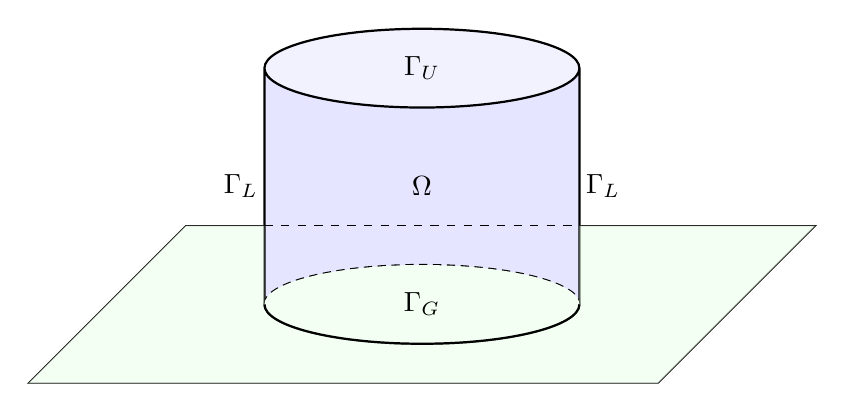
\begin{tikzpicture}
    \fill[color=blue!10] (2,0) -- (2,3) arc (360:180:2cm and 0.5cm) -- (-2,0) arc (180:360:2cm and 0.5cm);
    \fill[color=blue!5] (0,3) circle (2cm and 0.5cm);
    
    \draw[thick] (-2,3) -- (-2,0) arc (180:360:2cm and 0.5cm) -- (2,3) ++ (-2,0) circle (2cm and 0.5cm);
    \draw[densely dashed, thick] (-2,0) arc (180:0:2cm and 0.5cm);
    \draw (-2,1) -- (-3,1) --(-5,-1) -- (3,-1) -- (5,1) -- (2,1);
    \draw[dashed] (-2,1) -- (2,1);
    
    \fill[green!10,opacity=0.5] (-2,0) -- (-2,1) -- (-3,1) -- (-5,-1) -- (3,-1) -- (5,1) -- (2,1) -- (2,0) arc (0:180:2cm and -0.5cm);
    \fill[color=green!5] (0,0) circle (2cm and 0.5cm);
    
    \draw (0,1.5) node {$\Omega$};
    \draw (0,3) node {$\Gamma_U$};
    \draw (0,0) node {$\Gamma_G$};
    \draw (-2.3,1.5) node {$\Gamma_L$};
    \draw (2.3,1.5) node {$\Gamma_L$};
    
    \draw[thick] (2,0) arc (360:180:2cm and 0.5cm);
  \end{tikzpicture}
\end{figure}

Concerning the pollution concentration it is vital to choose boundary conditions that are physically as accurate as possible and at the same time not unnecessarily complicated. As we can see in many related papers, in the case of LAMs (limited area models) finding the right boundary conditions can be a nontrivial task.

In order to describe the boundary condition in a precise way we need to divide $\Gamma = \partial \Omega$ as follows. The upper boundary of the $\Omega$ domain is denoted by $\Gamma_U$, the lateral boundary is $\Gamma_L$, the lower boundary of the domain is $\Gamma_G,$ and for the collective $\Gamma_L \cup \Gamma_U$ section we use the notion $\Gamma_A$ (above the ground).
As we mentioned before, the case we are investigating is that of inland domains $\Omega$, i.e. the case of landscapes and cities with no significant nearby water surface.  This is very important since the boundary conditions for both wind velocity and pollution concentration in the air are different depending whether we are above solid ground or water surface. The boundary conditions we choose to use in the inland scenario are the following:

\begin{figure}[!h]
  \centering
  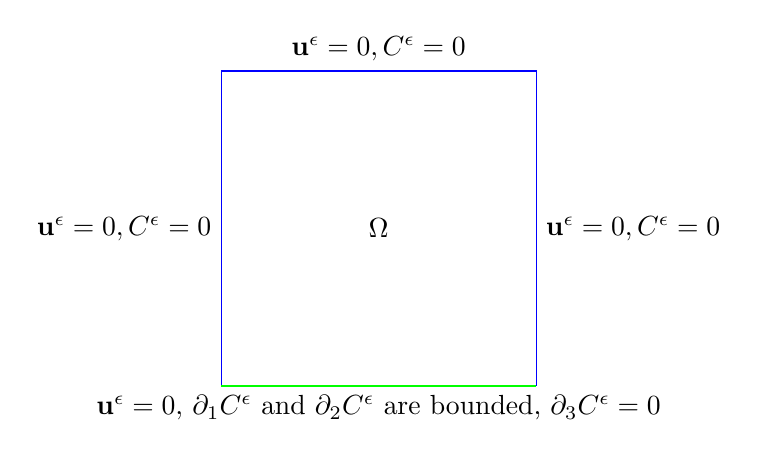
\begin{tikzpicture}
  
    \draw[blue] (0,0) -- (2,0) -- (4,0) -- (4,2) -- (4,4) -- (2,4) -- (0,4) -- (0,2) -- (0,0);
    \draw[green, thick] (0,0) -- (4,0);
    
    \draw (2,2)node{$\Omega$};
    \draw (2,0)node[below] {$\mathbf{u^\epsilon} = 0,$ $ \partial_1 C^\epsilon$ and $ \partial_2 C^\epsilon$ are bounded, $\partial_3 C^\epsilon = 0$};
    \draw (4,2)node[right] {$\mathbf{u^\epsilon} = 0, C^\epsilon=0 $};
    \draw (2,4)node[above] {$\mathbf{u^\epsilon} = 0, C^\epsilon=0 $};
    \draw (0,2)node[left] {$\mathbf{u^\epsilon} = 0, C^\epsilon=0 $};
    
  \end{tikzpicture}
\end{figure}

  \begin{itemize}
  
    \item The upper boundary $\Gamma_U$ of the domain we are considering is chosen to be at the isobar $z=h$ representing the planetary boundary layer (see \cite{arya2001introduction}), therefore we assume
    
    \begin{equation}
      \mathbf{u}^\epsilon_H = 0, \quad u^\epsilon_3 = 0, \quad C^\epsilon = 0 \quad \text{ on } \Gamma_U \times (0,T)
    \end{equation}
      
    \item On $\Gamma_L$ we use the same boundary conditions as on the upper level, i.e. we have
    
    \begin{equation}
      \mathbf{u}^\epsilon_H = 0, \quad u^\epsilon_3 = 0, \quad C^\epsilon = 0  \quad \text{ on } \Gamma_L \times (0,T).
    \end{equation}
    
    
    \begin{remark}
    If we wanted to use $C^\epsilon(x,y,z) = c$ with some $c$ constant value, we could make a change of variables distracting that background flow and arrive back to the same mathematical problem with $C$ being zero.
    \end{remark}
    \item In this model we neglect topological variations, and the $z=0$ plane represents the lower boundary. On the ground level we have
    
    \begin{equation}
      \mathbf{u}^\epsilon_H = 0, \quad u^\epsilon_3 = 0 \quad \text{ on } \Gamma_G \times (0,T) .
    \end{equation}
    
    This is the mathematical way of expressing no-slip boundary conditions for the horizontal wind speed and the impervious nature of the ground with respect to the wind. As for the concentration, the way we can choose ground level boundary conditions is the following. Firstly, we assume that the pollution is not absorbed by the ground, so we use
    
    $$\partial_3 C^\epsilon = 0 \text{ on } \Gamma_G$$
    
    (see also for example \cite{yeh1975three}). As we will see later in the case of the coastal domain, this condition can be relaxed without significantly effecting the proof. For the horizontal partial derivatives of the pollution, we require finiteness in the boundary norm, i.e. we have
    
    $$\partial_1 C^\epsilon, \partial_2 C^\epsilon \text{ are finite in } L^2 (0,T; \Gamma_G).$$
  
  \end{itemize}
  Specifically, for the pollution concentration reaching the ground level we use a similar approach as the one classically used for the wind traction reaching the top of the ocean (see for example \cite{azerad2001mathematical}, \cite{temam2005some}). We assume that the functions $\partial_1 C^\epsilon, \partial_2 C^\epsilon, \partial_3 C^\epsilon$ are equal to some sufficiently regular functions defined on the respective boundary. More accurately, we assume that we have $\nabla C^\epsilon = \boldsymbol{\sigma}$ on the lower boundary, where $\boldsymbol{\sigma} \in L^2(0,T;L^2(\Gamma_G))$, and the $\sigma_i$ terms denote the components of $\boldsymbol{\sigma}$. In particular in this inland case $\sigma_3$ is equal to zero on the $\Gamma_G$.
  
  Finally, the boundary conditions to describe the anisotropic system can be summarised as follows:
  
    \begin{equation} \label{ANSC8_coordinates_GFC}
      \begin{split}
        & \mathbf{u}^\epsilon = 0 \text{ on } \Gamma \times (0,T), \\
        &C^\epsilon = 0 \text{ on } ( \Gamma_U \cup \Gamma_L) \times (0,T), \\
        & \partial_1 C^\epsilon = \sigma_1, \partial_2 C^\epsilon = \sigma_2,\ \partial_3 C^\epsilon= 0 \text{ on } \Gamma_G \times (0,T), \\
        & \boldsymbol{\sigma} = (\sigma_1, \sigma_2, 0) \in L^2(0,T; \Gamma_G)\\
      \end{split} \raisetag{40pt}
    \end{equation}

Note that we have a domain where the lower and upper boundaries represent a physically existent layer (i.e. the ground and the planetary boundary layer), but outside the lateral boundary the physical world continues without influence and without any particular external condition. On boundaries of such nature we have to apply OBCs (open boundary conditions), which is not a trivial task, see for example \cite{wang2014ocean}. We need to avoid any spurious reflection or constraint which is unnatural, but at the same time we want the model to remain mathematically manageable.

If we assume $\mathbf{u}^\epsilon = O(1)$, then neglecting the $\epsilon^2$ and $\epsilon$ in the anisotropic equations, we formally arrive to the hydrostatic Navier-Stokes equations (i.e., primitive equations) combined with pollution.

    \begin{equation} \label{HNSC1_coordinates_GFC}    
    \partial_t u_1 + \mathbf{u} \cdot \nabla u_1 - \Delta_\nu u_1 -\alpha u_2 + \partial_1 p = 0 \text{ in } \Omega \times (0,T)
    \end{equation}
    
    \begin{equation} \label{HNSC2_coordinates_GFC}   
    \partial_t u_2 + \mathbf{u} \cdot \nabla u_2 - \Delta_\nu u_2 -\alpha u_1 + \partial_2 p = 0 \text{ in } \Omega \times (0,T)
    \end{equation}
    
    \begin{equation} \label{HNSC3_coordinates_GFC}   
    \partial_3 p = 0 \text{ in } \Omega \times (0,T)
    \end{equation}
    
    \begin{equation} \label{HNSC4_coordinates_GFC}   
    \nabla \cdot \mathbf{u} = 0 \text{ in } \Omega \times (0,T)
    \end{equation}
    
    \begin{equation} \label{HNSC5_coordinates_GFC}   
    \partial_t C + \mathbf{u} \cdot \nabla C = \nabla \cdot (\mathbf{M} \nabla C) + S \text{ in } \Omega \times (0,T)
    \end{equation}
    
    \begin{equation} \label{HNSC6_coordinates_GFC}   
    u_1 = u_2 = u_3 n_3 = 0 \text{ on } \Gamma \times (0,T)
    \end{equation}
    
    \begin{equation} \label{HNSC7_coordinates_GFC}   
    u_i (\cdot, t=0) = u_{0 i}, C (\cdot, t=0) = C_0 \text{ in } \Omega, \text{$i$ = 1,2}
    \end{equation}
    
    \begin{equation} \label{HNSC8_coordinates_GFC}
      \begin{split}
        &C = 0 \text{ on } ( \Gamma_U \cup \Gamma_L) \times (0,T), \\
        & \partial_1 C = \sigma_1, \partial_2 C = \sigma_2, \partial_3  C = 0, \boldsymbol{\sigma} = (\sigma_1, \sigma_2, 0) \in L^2(0,T; \Gamma_G)\\
      \end{split}
    \end{equation}
    
  \begin{remark} \label{sourceregularityremark}
    Here $S$ stands for the $\delta$ limit distribution. We keep the notation $S$ for generality, since as we will see later, instead of the approximated delta functions and the delta distribution, it is possible to use any sort of "sufficiently smooth" source term (which can be independent from $\epsilon$ in the anisotropic case as well) that is bounded in $L^2_t L^2_x.$
  \end{remark}

TODO where, instead of the originally used wind momentum equation, the hydrostatic air pressure assumption is used to describe the process in the vertical dimension. 

TODO This is a widely used coordinate system choice because in this specific system the rotation vector, and as a consequence, the Coriolis force takes a simpler form.

TODO We begin this part of this thesis by examining in detail what modifications and changes are necessary in the model so that we can prove a convergence theorem analogous to that formulated for weak solutions, but stated for the case of strong solutions this time.

%%% *** THE MODEL FOR THE POLLUTED ATMOSPHERE *** %%%
\subsection{The polluted atmosphere model in downwind-matching coordinates} \label{eqsdescribingatmpluspollution_dwmc}

The key point of this new model is to integrate some of the main ideas of the Gaussian plume dispersion model into the system describing the polluted atmosphere. Therefore we begin by fixing the local Cartesian coordinate system to be adjusted to the downwind direction, i.e. $z$ is oriented upwards, while $x$ is the downwind, and $y$ is the crosswind direction. Another assumption the Gaussian dispersion models typically use is that advection is more dominant than diffusion along the downwind direction, which leads to the appearance of an extra $\epsilon$ term in the concentration equation's Laplacian. Namely, we have

\begin{equation} \abs{u_1 \partial_{1} c} \gg | K_x \partial_{11} ^2 c | ,\end{equation}

which leads us to introducing the new scaling identity

\begin{equation} \label{ksepsk1} K_x = \epsilon K_1. \end{equation}

We use this diffusion rescaling result in addition to the original set of scaling equations described below. Every element of this latter set is a result of the shallowness of the domain, and they are applied in order to pass from the $\epsilon-$ dependent $\Omega^\epsilon$ original domain to the rescaled, $\epsilon-$free $\Omega$ domain.

Here the original $\Omega_\epsilon$ domain we consider is a local slice of the atmosphere written in Cartesian coordinates:

\begin{equation}
  \Omega_{\epsilon} = \{(x,y,z) \in \mathbb{R}^3 ; (x,y) \in \omega, 0 < z < \epsilon h(x,y) \},
\end{equation}

where $\omega$ is a Lipschitz-domain in $\mathbb{R}^2$, $h$ is a nonnegative Lipschitzian application.

In order to obtain the set of equations that describe the pollution phenomena in the atmosphere, we start with the original set of equations

\begin{equation} \label{originalEQ-V}
  \partial_t \mathbf{v} + (\mathbf{v} \cdot \nabla)\mathbf{v} -\Delta_{\nu} \mathbf{v} + \nabla q + 2 \mathbf{\omega} \times \mathbf{v}= \mathbf{g} \text{ in } \Omega_{\epsilon} \times (0,T)
\end{equation}
    
\begin{equation} \label{originalEQ-I}
  \nabla \cdot \mathbf{v} = 0 \text{ in } \Omega_{\epsilon} \times (0,T)
\end{equation}
    
\begin{equation} \label{diffusive}
  \partial_t P + \mathbf{v} \cdot \nabla P = \nabla \cdot (\mathbf{K} \nabla P) + Q \text{ in } \Omega_{\epsilon} \times (0,T),
\end{equation}

where the fluid velocity is denoted by $\mathbf{v}$ and the function $P$ represents the pollutant concentration. 

Each of these following scaling equations can be heuristically deduced from the typical physical dimension of the quantities (for more details see \cite{besson1992some}, \cite{azerad2001mathematical}, \cite{pollatmws2019}), unlike the previously presented equation ($\ref{ksepsk1}$), which is the effect of the coordinate choice itself. In detail, apart from the already introduced equation ($\ref{ksepsk1}$) we use the following scaling identities to arrive to the rescaled model.

\begin{equation} \label{shallownessscalingeqs}
  \begin{split}
    & x = x_1, \quad y = x_2, \quad z = \epsilon x_3, \\
    & v_1 = u_1^{\epsilon}, \quad v_2 = u_2^{\epsilon}, \quad v_3 = \epsilon u_3^{\epsilon}, \\
    & \nu_x = \nu_1, \quad \nu_y = \nu_2 , \quad \nu_z = \epsilon ^ 2\nu_3, \\
    & K_y = K_2 , \quad K_z = \epsilon^2 K_3, \\
    & P = \frac{1}{\epsilon} c^\epsilon, \quad Q = \frac{1}{\epsilon} s^\epsilon, \quad p = p^{\epsilon}
  \end{split}
\end{equation}

Once we apply the above scaling, we pass from the original $\Omega_\epsilon$ domain to the $\epsilon-$ independent

\begin{equation} \Omega =  \{(x_1,x_2,x_3) \in \mathbb{R}^3 ; (x_1,x_2) \in \omega, 0 < x_3 < h (x_1 , x_2) \} \end{equation}

set.

\begin{remark} \normalfont
  The inclusion of these new features related to the downwind-matching coordinate system in a pollution model are legitimate when the following circumstances hold:
  \begin{itemize}
    \item We are considering a time interval which is not "too long" --- meaning that it is reasonable to assume that we have a permanent, relatively stable main wind direction, i.e. fixing the horizontal coordinates makes sense in the first place.
    \item There is an adequate, relatively high wind speed --- low wind speeds in general lead to a situation where three dimensional diffusion dominates, leading to an error caused by the dominant advection assumption. Fast changing wind direction and low windspeed resulting in fast pollutant settling can make it extremely challenging to obtain reliable results from Gaussian models.
  \end{itemize}
\end{remark}

Choosing the coordinate system in this particular way results in changes in three main points of the system with respect to the case of the rotating geophysical frame. One of these is the Coriolis term, since now the $x$ axis is not necessarily perpendicular to the rotation vector. We need to revisit the boundary conditions as well, and as discussed above, a modification in the pollution concentration equation also has to be taken into account. We will describe these changes and their consequences in detail --- the main challenge in proving this section's convergence results is in fact to handle the effect of this latter change in the inequalities that provide boundedness for the required quantities.

\begin{remark} \normalfont
For clarity, we add a comment here regarding the intuitive meaning of what we understand by the downwind direction $\mathbf{x}$ (which gives orientation to a coordinate axes), and the velocity $\mathbf{v}$ itself (which is the solution function). The downwind direction is an approximately steady-in-time direction, it can be seen as the direction marked by the wind direction trackers on an airport or meteorological point. When we consider the downwind, we neglect the small perturbations in its orientation, it can be viewed as a time-averaged direction as long as the fluctuation is relatively small. On the other hand, the velocity itself is a three-dimensional, time dependent vector that changes second after second.
\end{remark}

To expand the $2 \mathbf{\omega} \times \mathbf{v}$ Coriolis term, firstly it is necessary to understand the structure of the new rotation vector. Note that the downwind-matching coordinate system and the original east-north-upwards oriented system are different only in a rotation around the $z$ axis. Let $\theta$ denote the angle between the respective $x$ axes, $\phi$ denotes the latitude, then the rotation vector expressed in the downwind-matching coordinate system becomes

\begin{gather}
 \begin{bmatrix} \cos(\theta) & -\sin(\theta) & 0 \\ \sin(\theta) & \cos(\theta) & 0 \\ 0 & 0 & 1 \end{bmatrix} \begin{bmatrix} 0 \\ f \cos(\phi) \\ f \sin(\phi) \end{bmatrix}
 =
  f \begin{bmatrix} -\sin(\theta)\cos(\phi) \\ \cos(\theta) \cos(\phi) \\ \sin(\phi) \end{bmatrix}.
\end{gather}

Now, let

$$\alpha = -2 f \sin(\theta)\cos(\phi), \quad \beta = 2 f \cos(\theta) \cos(\phi), \quad \gamma = 2 f \sin(\phi),$$

i.e. $2 \omega = (\alpha, \beta, \gamma),$ then using this, the Coriolis force takes the form

\begin{gather}
\begin{bmatrix} \alpha \\ \beta \\ \gamma \end{bmatrix}
 \times
 \begin{bmatrix} u_1 \\ u_2 \\ \epsilon u_3 \end{bmatrix}
 =
 \begin{bmatrix}  \beta \epsilon u_3 - \gamma u_2 \\ \gamma u_1 - \alpha \epsilon u_3  \\ \alpha u_2 - \beta u_1 \end{bmatrix}.
\end{gather}

Thus, these are the terms that appear in the three velocity equations below; but note that in the rescaled version of the vertical velocity equation the third component of the Coriolis term is present with an $\epsilon$ multiplier, which is obtained from the $\epsilon$ term in the denominator of $\partial_z p.$

Using the expanded form of the Coriolis terms and applying the scaling process ($\ref{shallownessscalingeqs}$) combined with $(\ref{ksepsk1}),$ we arrive to the merged anisotropic equations of the polluted atmosphere above inland surface:
  
    \begin{equation} \label{ANSC1_coordinates_DWMC}
    \partial_t u^\epsilon _1 + \mathbf{u}^\epsilon \cdot \nabla u^\epsilon _1 -\Delta_\nu u^\epsilon _1 -\gamma u_2^\epsilon + \epsilon \beta u_3^\epsilon + \partial_1 p^\epsilon = 0 \text{ in } \Omega \times (0,T)
    \end{equation}
    
    \begin{equation} \label{ANSC2_coordinates_DWMC}
    \partial_t u_2^\epsilon + \mathbf{u}^\epsilon \cdot \nabla u_2^\epsilon -\Delta_\nu u_2^\epsilon + \gamma u_1^\epsilon - \alpha \epsilon u^\epsilon_3  + \partial_2 p^\epsilon = 0 \text{ in } \Omega \times (0,T)
    \end{equation}
    
    \begin{equation} \label{ANSC3_coordinates_DWMC}
    \epsilon^2 \{  \partial_t u_3^\epsilon + \mathbf{u}^\epsilon \cdot \nabla u_3^\epsilon -\Delta_\nu u_3^{\epsilon} \} + \epsilon \alpha u^\epsilon_2 - \epsilon \beta u_1^\epsilon + \partial_3 p^\epsilon = 0 \text{ in } \Omega \times (0,T)
    \end{equation}
    
    \begin{equation} \label{ANSC4_coordinates_DWMC}
    \nabla \cdot \mathbf{u}^\epsilon= 0 \text{ in } \Omega \times (0,T)
    \end{equation}
    
    \begin{equation} \label{ANSC5_coordinates_DWMC}
    \partial_t c^\epsilon + \mathbf{u^\epsilon} \cdot \nabla c^\epsilon = \epsilon K_1 \partial_{11} ^ 2 c^\epsilon + K_2 \partial_{22} ^ 2 c^\epsilon + K_3 \partial_{33} ^ 2 c^\epsilon + s^\epsilon \text{ in } \Omega \times (0,T).
    \end{equation}

The initial condition for the velocity and the pollution concentration are
    
    \begin{equation} \label{ANSC6_coordinates_DWMC}
    \mathbf{u}^\epsilon (\cdot, t = 0) = \mathbf{u}_0, \quad c^\epsilon (\cdot, t=0) = c_0  \quad \text{ in } \Omega.
    \end{equation}
  
We will specify the regularity of the initial data in Sections \ref{sectionWS} and \ref{sectionSTRONGsol} according to the fact whether we are dealing with weak or strong solutions.

This system will become complete when we define the boundary conditions --- we describe these in detail in Sections \ref{sectionWS} and \ref{sectionSTRONGsol} as they are chosen with different considerations depending on the type of the solutions we are dealing with.

If we assume $\mathbf{u}^\epsilon = O(1)$, then neglecting the $\epsilon^2$ and $\epsilon$ including terms in the anisotropic equations, we formally arrive to the hydrostatic Navier-Stokes equations (i.e. primitive equations) combined with pollution.

    \begin{equation} \label{HNSC1_coordinates_DWMC}    
    \partial_t u_1 + \mathbf{u} \cdot \nabla u_1 - \Delta_\nu u_1 -\gamma u_2 + \partial_1 p = 0 \text{ in } \Omega \times (0,T)
    \end{equation}
    
    \begin{equation} \label{HNSC2_coordinates_DWMC}   
    \partial_t u_2 + \mathbf{u} \cdot \nabla u_2 - \Delta_\nu u_2 + \gamma u_1 + \partial_2 p = 0 \text{ in } \Omega \times (0,T)
    \end{equation}
    
    \begin{equation} \label{HNSC3_coordinates_DWMC}   
    \partial_3 p = 0 \text{ in } \Omega \times (0,T)
    \end{equation}
    
    \begin{equation} \label{HNSC4_coordinates_DWMC}   
    \nabla \cdot \mathbf{u} = 0 \text{ in } \Omega \times (0,T)
    \end{equation}
    
    \begin{equation} \label{HNSC5_coordinates_DWMC}   
    \partial_t c + \mathbf{u} \cdot \nabla c = K_2 \partial_{22} ^ 2 c + K_3 \partial_{33} ^2 c + s \text{ in } \Omega \times (0,T)
    \end{equation}
    
    \begin{equation} \label{HNSC6_coordinates_DWMC}   
    u_i (\cdot, t=0) = u_{0 i}, \quad c (\cdot, t=0) = c_0 \text{ in } \Omega, \text{$i$ = 1,2}
    \end{equation}
    
The specific definitions of the $s^\epsilon$ and $s$ source terms also depend on whether we consider weak or strong solutions. In both cases they are fundamentally based on the notion of the nascent delta function with parameter $\epsilon$ and the delta distribution, but their exact definitions will be given in the subsections according to the regularity of the solutions.

To conclude the description of the model we highlight an important feature of the system that is suggested also by the structure of the governing equations (\ref{ANSC5_coordinates_DWMC}) and (\ref{HNSC5_coordinates_DWMC}). With respect to pollution diffusion, directions $y$ and $z$ have a particular and shared importance compared to the $x$ direction, namely that we have diffusion taking place on $\mathcal{O}(1)$ scale in the former ones. This suggests the introduction of the generalised direction $d$ which includes directions $y$ and $z$ (similarly to the more standard concept of $h$ standing for the horizontal directions $x$ and $y$). Furthermore, we accordingly introduce the notations $\Delta_d = K_2 \partial_{22}^2 + K_3 \partial_{33}^2$ and $\nabla_d = (\partial_2, \partial_3).$

The following two sections are dedicated to state and prove a rigorous connection on the level of solutions between the anisotropic and hydrostatic models described above. Section \ref{sectionWS} focuses on the verification of a convergence result between the models (\ref{ANSC1_coordinates_DWMC})-(\ref{ANSC6_coordinates_DWMC}) and (\ref{HNSC1_coordinates_DWMC})-(\ref{HNSC6_coordinates_DWMC}) in the framework of weak solutions. In Section \ref{sectionSTRONGsol} we apply stronger initial regularities and -- from the computations' point of view -- a more favourable boundary structure: here we describe an analogous result to that in Section \ref{sectionWS}, but the statement holds for strong solutions.

TODO The theorem we will migrate between these two coordinate systems is focused on the polluted atmosphere as a shallow domain. Incorporating the shallowness into the model via introducing the $$\epsilon = \frac{\text{characteristic depth}}{\text{characteristic width}}$$ shallowness parameter we have proved the theoretical correctness of the hydrostatic approximation for the combination of a three-dimensional velocity function and a pollution concentration function. Specifically, we have showed that any weak solution of the shallow polluted atmosphere converges weakly to a weak solution of the so-called primitive equations representing the hydrostatic limit model. In the first part of this chapter our goal is to verify an analogous version of this convergence theorem for the case of the more considerately chosen downwind-matching coordinate system. 

TODO The downwind-matching coordinate system and the set of modelling equations we work with are essentially identical to those defined in part one --- what separates the two main sections is the quality of the convergence we are able to state.

\chapter{The asymptotic behaviour of the anisotropic solutions in geophysical coordinates}\label{geophysicalchapter}

%%% *** WEAK FORMULATION AND MAIN RESULT*** %%%
\section{Weak formulation and Main Result} \label{weakformulationmainresult}

In this section we describe the weak formulation of the merged equations in both the anisotropic and hydrostatic case we are going to use in the thesis, and we state our main result.
  
  We need to define the following spaces:
  
  \[ C^{\infty}_{\Gamma_A} (\Omega) = \{ \varphi \in C^\infty (\bar{\Omega}); \varphi = 0 \text{ on some neighbourhood of } \Gamma_A \} \]
  
  \[ H^k_{\Gamma_A} (\Omega) = \overline{C_\Gamma ^ \infty (\Omega)} ^ {H^k (\Omega)} = \{ v \in H^k(\Omega); v=0 \text{ on } \Gamma_A \} \]
  
  \[ \mathbf{V} = \{ \mathbf{v} \in  H^1_{\Gamma_A} (\Omega) \times H^1_{\Gamma_A} (\Omega) \times H^1_0 (\Omega); \nabla \cdot \mathbf{v} = 0 \text{ in } \Omega \} \]
  
  \[ H (\partial_3, \Omega) = \{ v \in L^2(\Omega); \partial_3 v \in L^2 (\Omega)\} \]
  
  \[ H_0 (\partial_3, \Omega) = \overline{C_0 ^\infty (\Omega)}^{H (\partial_3, \Omega)} = \{ v \in H(\partial_3, \Omega); v n_3 = 0 \text{ on } \Gamma \} \]
  
  \[ \mathbf{W} = \{ \mathbf{u} \in  H^1_{\Gamma_A} (\Omega) \times H^1_{\Gamma_A} (\Omega) \times H_0 (\partial_3, \Omega); \nabla \cdot \mathbf{u} = 0 \text{ in } \Omega \} \]
  
  Then the weak formulation of the hydrostatic system (\ref{HNSC1_coordinates_GFC}) - (\ref{HNSC8_coordinates_GFC}) takes the following form.
  
  \begin{definition} \label{definitionhydrostaticWF}
  
  Find $(\mathbf{u}, C)$ such that $\mathbf{u} = (\mathbf{u}_H, u_3) \in L^2 (0, T; \mathbf{W})$ with $\mathbf{u}_H \in L^\infty (0,T; L^2(\Omega)^2),$ and $C \in L^\infty(0,T; L^2(\Omega))$ with $C \in L^2(0,T; H^1(\Omega))$, such that
  
  \begin{equation}
    \begin{split}
      & \int_0^T \bigg[ -(\mathbf{u}_H, \partial_t \mathbf{\tilde{u}}_H) + (\nabla_\nu \mathbf{u}_H, \nabla_\nu \mathbf{\tilde{u}}_H) - (\mathbf{u}_H, (\mathbf{u} \cdot \nabla) \mathbf{\tilde{u}}_H) + (b(\mathbf{u}_H), \mathbf{\tilde{u}}_H) \bigg ] \diff t \\
      & = (\mathbf{u}_{0H}, \mathbf{\tilde{u}}_H(0)) \diff t \raisetag{15pt}\label{hydrostaticWF_U}
    \end{split}
  \end{equation}
  
  and
  
    \begin{equation}
    \begin{split}
      & \int_0^T \bigg[ -(C, \partial_t \tilde{C}) -(\mathbf{u}C, \nabla \tilde{C}) +  (\mathbf{M} \nabla C, \nabla \tilde{C}) - \int_{\Gamma_G} \boldsymbol{\sigma} \mathbf{M} \tilde{C} \vec{\boldsymbol{n}}_{\Gamma_G} \bigg ] \diff t \\
      & = (C(0), \tilde{C}(0)) + \int_0^T (S,\tilde{C}) \diff t \raisetag{20pt} \label{hydrostaticWF_C}
    \end{split}
  \end{equation}
  
  for all $(\mathbf{\tilde{u}}, \tilde{C})$ with $\mathbf{\tilde{u}} = (\mathbf{\tilde{u}}_H, \tilde{u}_3) \in H^1 (0,T, \mathbf{W})$, $\mathbf{\tilde{u}}_H (T) = 0$ and $\partial_3 \mathbf{\tilde{u}}_H \in L^\infty (0, T; L^3 (\Omega)^2)$ and  $\tilde{C} \in L^2 (0,T, H^2_{\Gamma_A} (\Omega)) \cap H^1 (0,T, L^2)$, $\tilde{C} (T) = 0$. 
  
  \end{definition}
  
  Note that the term $\int_0^T (S,\tilde{C}) \diff t$ makes sense since in this case $S$ denotes the delta distribution and we have 
  
  \[ (S,\tilde{C}) = \int_\Omega \delta(\mathbf{x} - \mathbf{x}_s) \tilde{C}(\mathbf{x}) \diff \mathbf{x} = \tilde{C}(\mathbf{x}_s).\]
  
  The existence of weak solution for the hydrostatic system (\ref{HNSC1_coordinates_GFC}) - (\ref{HNSC8_coordinates_GFC}) can be proved in the spirit of \cite{temam2005some}. In appendix A we will outline the main steps of the proof and the differences compared to the ocean model.

  The weak form of the anisotropic system is as follows.
  
  \begin{definition} \label{definitionanisotropicWF}
  
  Find $\mathbf{u}^\epsilon = (\mathbf{u}^\epsilon_H, u^\epsilon_3) \in L^2 (0,T ; \mathbf{V}) \cap L^\infty (0, T; L^2 (\Omega)^3)$ and $C^\epsilon \in L^\infty (0,T; L^2(\Omega)) \cap L^2 (0,T; H^1(\Omega))$, such that
  
  \begin{equation}
    \begin{split}
      & \int_0^T \bigg [ -(\mathbf{u}^\epsilon_H, \partial_t \mathbf{\tilde{u}}_H) + (\nabla_\nu \mathbf{u}^\epsilon_H, \nabla_\nu \mathbf{\tilde{u}}_H) - (\mathbf{u}^\epsilon_H, (\mathbf{u}^\epsilon \cdot \nabla) \mathbf{\tilde{u}}_H) + (b(\mathbf{u}^\epsilon_H), \mathbf{\tilde{u}}_H) \bigg ] \diff t \\
      & + \epsilon \beta \int_0 ^ T \big [ (u_3 ^\epsilon, \tilde{u}_1) - (u_1^\epsilon, \tilde{u}_3) \big ] \diff t\\
      & + \epsilon^2 \int _0 ^ T \big [ -(u_3^\epsilon, \partial_t \tilde{u}_3) +(\mathbf{u}^\epsilon \cdot \nabla u_3 ^ \epsilon, \tilde{u}_3) + (\nabla_\nu u_3^\epsilon, \nabla_\nu \tilde{u}_3) \big ] \diff t \\
      & = (\mathbf{u}^\epsilon_{0H}, \mathbf{\tilde{u}}_H(0)) + \epsilon^2 (u_{03}^\epsilon, \tilde{u}_3 (0)) \diff t \raisetag{20pt} \label{anisotropicWF_U}
    \end{split}
  \end{equation}
  
  and
  
    \begin{equation}
    \begin{split}
      & \int_0^T \bigg [ -(C^\epsilon, \partial_t \tilde{C}) -(\mathbf{u}^\epsilon C^\epsilon, \nabla \tilde{C}) + (\mathbf{M} \nabla C^\epsilon, \nabla \tilde{C}) - \int_{\Gamma_G} \boldsymbol{\sigma} \mathbf{M} \tilde{C} \vec{\boldsymbol{n}}_{\Gamma_G} \bigg ] \diff t \\
      & =  (C^\epsilon (0), \tilde{C} (0)) + \int_0^T (S^\epsilon,\tilde{C}) \diff t \raisetag{20pt} \label{anisotropicWF_C}
    \end{split}
  \end{equation}
  
  for all $\mathbf{\tilde{u}} = (\mathbf{\tilde{u}}_H, \tilde{u}_3) \in H^1 (0,T;\mathbf{V})$ with $\mathbf{\tilde{u}}(T) = 0$ and $\tilde{C}$ such that $\tilde{C} \in H^1 (0,T, H^2_{\Gamma_A} (\Omega))$ and $\tilde{C} (T) = 0$.
  
  \end{definition}
  
  Note that since in our case the source term $S^\epsilon$ is given by (\ref{approxsourceterm}), the last term in (\ref{anisotropicWF_C}) is well defined. If we use a source function of a different and more general form, it needs to satisfy the $L_t^2 L_x^2$ boundedness criteria for the weak formulation to make sense.

We will omit the proof of the existence of weak solutions (see Definition \ref{definitionanisotropicWF}.) for the anisotropic system (\ref{ANSC1_coordinates_GFC}) - (\ref{ANSC8_coordinates_GFC}) since it follows by standard finite-dimensional Galerkin approximation.

Now we are ready to state our main result.
  
\begin{theorem} \label{maintheorem}
  Let $\mathbf{u}_0$ $\in$ $L^2 (\Omega)^3$, with $\nabla \cdot \mathbf{u}_0 = 0, \mathbf{u}_0 \cdot \mathbf{n} = 0$ on $\partial \Omega$; let $C_0 \in$ $L^2 (\Omega)$, $C_0 = 0$ on $ \partial \Omega$, and assume that the boundary conditions (\ref{ANSC8_coordinates_GFC}) hold; then as the aspect ratio $\epsilon$ tends to zero, any weak solution $(\mathbf{u}^\epsilon, C^\epsilon)$ of the anisotropic equations (\ref{ANSC1_coordinates_GFC}) - (\ref{ANSC5_coordinates_GFC}) converge to a weak solution $(\mathbf{u}, C)$ of the hydrostatic equations of the polluted atmosphere (\ref{HNSC1_coordinates_GFC}) - (\ref{HNSC5_coordinates_GFC}).
\end{theorem}

%%% *** PROOF *** %%%
\section{Proof of the main theorem} \label{proof}
 
 This section is devoted to the proof of Theorem \ref{maintheorem}. In the extended case with the pollution equation the proof relies on a priori estimates gained from the energy inequality and, as we will see this is sufficient to pass to the limit in the linear terms. Concerning the nonlinear terms we will prove a uniform in $\epsilon$ space time estimate for $\mathbf{u}^\epsilon$ and $C^\epsilon$ that will allow us to apply a compactness criterion proved in \cite{azerad2001mathematical}.

  \subsection{Energy inequality}
  
  As we mentioned before, one of the most fundamental tools in this proof is the energy inequality. If we calculate it for the anisotropic system, we obtain that for a.e. $t \in [0,T]$ the following holds:
  
  \begin{equation}
    \begin{split}  
    & \frac{1}{2} (\norm{\mathbf{u}_H^\epsilon (t)}_{L^2}^2 + \epsilon ^ 2 \norm{u_3^\epsilon (t)}_{L^2}^2 + \norm{C^\epsilon (t)}_{L^2}^2) + \int_0 ^ t \big[ \norm{\nabla_\nu \mathbf{u}_H^\epsilon}_{L^2}^2 + \epsilon ^ 2 \norm{\nabla_\nu u_3^\epsilon}_{L^2}^2  \big] \diff \tau \\
    & + \int_0 ^ t  (\mathbf{M} \nabla C^\epsilon, \nabla C^\epsilon) d \tau \\
    & \leq \int_0^t (S^\epsilon,C^\epsilon) \diff \tau + \frac{1}{2} (\norm{\mathbf{u}_H^\epsilon (0)}_{L^2}^2 + \epsilon ^ 2 \norm{u_3^\epsilon (0)}_{L^2}^2 + \norm{C^\epsilon_0}_{L^2}^2) \\
    & + \int _ 0 ^ t  \int_{\Gamma_G} ((\nabla C^\epsilon) \mathbf{M}) C^\epsilon \vec{\mathbf{n}}_{\Gamma_G}  \diff \tau \\
    & = I_1 + I_2 + I_3. \raisetag{70pt} \label{energyIEQ}
    \end{split}
  \end{equation}    
  
  From the hypothesis on the initial data and since the $S^\epsilon$ source term is in $L^\infty_x (\Omega)$, $I_1$ and $I_2$ are bounded. The only terms we need to work on further are the expressions in $I_3$.
  
  By using the H\"older inequality and the generalised Young inequality for any $\zeta > 0,$ we can estimate this term in the following way.
  
  \begin{equation}
    \begin{split}  \label{boundI_3}
    I_3 & = \int _ 0 ^ t \int_{\Gamma_G} \sum_{i=1}^3 \bigg( \big(\sum_{j=1}^3 M_{ij} \partial_j C^\epsilon \big) C^\epsilon \mathbf{n}_{\Gamma_G, i} \bigg) \diff \tau \\
    & \leq \sum_{i,j = 1}^3 M_{ij} \int _ 0 ^ t \norm{\partial_i C^\epsilon}_{L^2 (\Gamma_G)}  \norm{C^\epsilon}_{L^2 (\Gamma_G)} \diff \tau \\
    & \leq \sum_{i,j = 1}^3 \frac{1}{\zeta} M_{ij} \frac{1}{2} \int_0 ^ t \norm{\partial_i C^\epsilon}^2 _{L^2 (\Gamma_G)} \diff \tau + \zeta M_{ij} \int_0 ^ t \frac{1}{2} \norm{C^\epsilon}^2 _{L^2 (\Gamma_G)} \diff \tau \\
    & \leq \sum_{i,j = 1}^3 \frac{1}{\zeta} M_{ij} \frac{1}{2} \int_0 ^ t \norm{\partial_i C^\epsilon}^2 _{L^2 (\Gamma_G)} \diff \tau + \zeta \frac{1}{2} M_{ij} c_T \int_0 ^ t \norm{C^\epsilon}^2 _{W^{1,2} (\Omega)} \diff \tau \\
    & \leq \sum_{i,j = 1}^3 \bigg( \frac{1}{\zeta} M_{ij} \frac{1}{2} \int_0 ^ t \norm{\partial_i C^\epsilon}^2 _{L^2 (\Gamma_G)} \diff \tau + \zeta \frac{1}{2} M_{ij} c_T  \int_0 ^ t \norm{\nabla C^\epsilon}^2 _{L^2 (\Omega) }  \diff \tau \\
    & + \zeta \frac{1}{2} M_{ij} c_T  \int_0 ^ t \norm{C^\epsilon}^2 _{L^2 (\Omega) } \diff \tau \bigg), \raisetag{30pt}
    \end{split}
  \end{equation}  
  
  where the $c_T$ constant is provided by the trace theorem, and the boundary term is bounded because of the a priori assumptions made on the boundary conditions.
  
   After applying the coercivity property (\ref{coercivity}) of the diffusion matrix, (\ref{energyIEQ}) now takes the form of the following energy inequality,

  \begin{equation}
    \begin{split}  
    & \frac{1}{2} (\norm{\mathbf{u}_H^\epsilon (t)}_{L^2}^2 + \epsilon ^ 2 \norm{u_3^\epsilon (t)}_{L^2}^2 + \norm{C^\epsilon (t)}_{L^2}^2) + \int_0 ^ t \big [\norm{\nabla_\nu \mathbf{u}_H^\epsilon}_{L^2}^2 + \epsilon ^ 2 \norm{\nabla_\nu u_3^\epsilon}_{L^2}^2 \big ] \diff \tau \\
    & + \int_0 ^ t \bigg[ (\lambda - \sum_{i,j = 1}^3 \zeta \frac{1}{2} M_{ij} c_T) \norm{\nabla C^\epsilon}_{L^2}^2  \bigg] \diff \tau \\
    & \leq \sum_{i,j = 1}^3 \frac{1}{\zeta} M_{ij} \frac{1}{2} \int_0 ^ t \norm{\sigma_i}^2 _{L^2 (\Gamma_G)} \diff \tau + \frac{1}{2} (\norm{\mathbf{u}_H^\epsilon (0)}_{L^2}^2 + \epsilon ^ 2 \norm{u_3^\epsilon (0)}_{L^2}^2 + \norm{C^\epsilon (0)}_{L^2}^2) \\
    & + \int_0^t (S^\epsilon,C^\epsilon) \diff \tau + \sum_{i,j = 1}^3 \zeta \frac{1}{2} M_{ij} c_T  \int_0 ^ t \norm{C^\epsilon}^2 _{L^2 (\Omega) } \diff \tau. \raisetag{90pt} \label{finalformEIEQ}
    \end{split}
  \end{equation}  
    
  It is now straightforward to see that the coefficients of the pollution terms are positive, since the $\zeta = \zeta(\lambda)$ constant of the generalised Young inequality can be freely chosen in a way such that the requirement $(\lambda - \sum \zeta \frac{1}{2} M_{ij} c_T) > \lambda/2 > 0$ is satisfied.
    
  \subsection{A priori estimates and weak convergence}
  
  From the final form of the energy inequality we obtain uniform a priori estimates that we summarise in the following proposition.
  
  \begin{prop}
    Let $u^\epsilon_1, u^\epsilon_2, u^\epsilon_3$ and $C^\epsilon$ be the weak solutions of the system (\ref{ANSC1_coordinates_GFC}) - (\ref{ANSC5_coordinates_GFC}) in the sense of Definition \ref{definitionanisotropicWF}. Then it holds,
    
    \begin{align}
      & u^\epsilon_1, u^\epsilon_2, \epsilon u^\epsilon_3, C^\epsilon & \quad & \text{are bounded in $L^\infty (0,T; L^2(\Omega)),$} \label{proposition1} \\
      & u^\epsilon_3 & \quad & \text{is bounded in $L^2 (0,T; L^2(\Omega)),$} \label{propositionExtra} \\
      & u^\epsilon_1, u^\epsilon_2, \epsilon u^\epsilon_3 & \quad & \text{are bounded in $L^2(0,T; H^1(\Omega)),$} \label{proposition2} \\
      & C^\epsilon & \quad & \text{is bounded in $L^2(0,T;H^1(\Omega)).$} \label{proposition3}
    \end{align}
    
  \end{prop}
  
  \begin{proof}
  By applying the classical Gr\"onwall inequality, (\ref{proposition1}), (\ref{proposition2}) and (\ref{proposition3}) follow directly by the energy inequality (\ref{finalformEIEQ}). On the other hand, (\ref{propositionExtra}) can be verified by using the divergence free condition and that as a consequence, we have $\partial_3 u_3 = - \partial_1 u_1 - \partial_2 u_2$ bounded in $L^2_t L^2 _x$. The bound holds for $u_3$ itself as well, owing to the Poincar\'e inequality in the vertical direction, and using that $u_3$ vanishes on the boundary.
  \end{proof}
  
  As a consequence, up to subsequences still denoted by the same way, we have the following weak convergence results.
  
  \begin{align} 
    &  \mathbf{u}_H^\epsilon \rightharpoonup \mathbf{u}_H &\quad & \text{weakly in $L_t^\infty L_x^2 \cap L_t^2 H_x^1$,} \label{WeakConvUHEps} \\
    &  \epsilon^2 u_3^\epsilon \to 0 &\quad & \text{strongly in $L_t^\infty L_x^2 \cap L_t^2 H_x^1$,} \label{WeakConvU3Eps} \\ 
    & u_3^\epsilon \rightharpoonup u_3  &\quad & \text{weakly in $L_t^2 L_x^2$,} \label{WeakConvU3NoEps} \\
    & C^\epsilon \rightharpoonup C &\quad & \text{weakly in $L_t^\infty L_x^2 \cap L_t^2 H_x^1$} \label{WeakConvCEps1}
  \end{align} 

\subsection{Passing to the limit}

    In order to conclude the proof of Theorem \ref{maintheorem} we pass to the limit in the weak formulation (\ref{anisotropicWF_U})-(\ref{anisotropicWF_C}). To take the limit for the linear velocity terms that do not include the concentration function $C^\epsilon$ we can use (\ref{WeakConvUHEps}), (\ref{WeakConvU3Eps}) and (\ref{WeakConvU3NoEps}), and the bounds (\ref{propositionExtra}), (\ref{proposition2}). As for the nonlinear terms, the convergence can be shown using a time compactness theorem that is based on a result by Simon \cite{simon1986compact}. The key point is to apply a sort of generalisation of the classical translation criterium of Riesz-Frechet-Kolmogorov which enables us to get strong convergence for the horizontal velocities. This is achieved by establishing a bound for the perturbation of $\mathbf{u}_H$ of the form $\norm{\tau_h \mathbf{u}_H - \mathbf{u}_H}_{L^p(0,T-h, \mathbf{Y})} \leq \varphi(h) + \psi(\epsilon),$ where $\mathbf{Y}$ is a Banach space, $\varphi$ and $\psi$ are appropriate functions with their limits vanishing at zero, and $\tau_h \mathbf{u}_H = \mathbf{u}_H (t+h) $. After obtaining strong convergence for $\mathbf{u}_H,$ the proof of the convergence for these nonlinear terms can be closed by applying basic interpolation techniques and the generalised H\"older inequality. The details are omitted since they are analogous to those described in \cite{azerad2001mathematical}.
  
    For the linear terms including the concentration $C^\epsilon$ we can directly apply the weak convergence result of (\ref{WeakConvCEps1}).
    
    We get
    
    \[ \int_0 ^ T (C^\epsilon , \partial_t \tilde{C}) d \mathrm{t} \to \int_0^T (C, \partial_t \tilde{C}) \diff t,\]
    
    \[ \int_0 ^ T  (\mathbf{M} \nabla C^\epsilon, \nabla \tilde{C}) d \mathrm{t} \to \int_0^T (\mathbf{M} \nabla C, \nabla \tilde{C}) \diff t.\]
      
    For the source term, by applying standard results for distribution functions, we get $(S^\epsilon, \tilde{C}) \to  (S, \tilde{C}).$ 
      
Finally we have to deal with the nonlinear term $(\mathbf{u}^\epsilon C^\epsilon, \nabla \tilde{C}).$
  
By analysing this nonlinear term in a more precise way we see that $u^\epsilon_i C^\epsilon$ for $i=1,2$ is weakly convergent since as we mentioned before, we have the strong convergence of the horizontal velocities, while in the case of $i=3$ this property does not hold. We overcome this difficulty by proving a compactness property for the pollution concentration $C^\epsilon.$ The key tool will be the following compactness criterion (for the proof see Theorem 5.1 in \cite{azerad2001mathematical}).

\begin{theorem}
Let $T>0,$ and let the Banach spaces $\mathbf{X} \hookrightarrow \mathbf{B} \hookrightarrow \mathbf{Y},$ where $\mathbf{X}$ is compactly embedded in $\mathbf{B},$ and $\mathbf{B}$ is continuously embedded in $\mathbf{Y}.$ Let $(f_\epsilon)_{\epsilon>0}$ be a family of functions of $L^p (0,T; \mathbf{X}), 1 \leq p \leq \infty,$ with the extra condition $(f_\epsilon)_{\epsilon>0} \subset C (0,T; \mathbf{Y})$ if $p = \infty,$ such that
\begin{enumerate}
  \item $(f_\epsilon)_{\epsilon>0}$ is bounded in $L^p (0,T; \mathbf{X}),$
  \item $\norm{\tau_h f_\epsilon - f_\epsilon}_{L^p(0,T-h; \mathbf{Y})} \leq \varphi(h) + \psi(\epsilon)$ with
  $$
    \begin{cases}
      \lim_{h \to 0} \varphi(h) = 0,\\
      \lim_{\epsilon \to 0} \psi(\epsilon) = 0.
    \end{cases}
  $$
  \end{enumerate}
  
Then the family $(f_\epsilon)_{\epsilon>0}$ possesses a cluster point in $L^p (0,T; \mathbf{B})$ and also in $\mathcal{C}(0,T; \mathbf{B})$ if $p = \infty$ as $\epsilon \to 0.$
\end{theorem}

We will be able to apply the statement of this theorem for $p=2$ and the spaces $H^1 \hookrightarrow L^2 \hookrightarrow {H^2}^*,$ where ${H^2}^*$ is the dual of ${H^2}$, obtaining that

\[C^\epsilon \to C \text{ strongly in } L^2_t L^2_x,\]

and thus we have the weak convergence result $u^\epsilon_3 C^\epsilon \rightharpoonup u_3 C.$

In the following we will verify that the theorem's conditions hold for our choice of spaces and $p$. Since (\ref{proposition3}) is already given, we only have to show the bound $\norm{\tau_h C^\epsilon - C^\epsilon}_{L^2(0,T-h, {H^2}^*)} \leq \varphi(h) + \psi(\epsilon)$ in order to close the argument regarding the weak convergence of $u^\epsilon_3 C^\epsilon$.

\begin{prop}
The estimate $\norm{\tau_h C^\epsilon - C^\epsilon}_{L^2(0,T-h, {H^2}^*)} \leq c \cdot h^{1/4}$ holds.
\end{prop}

\begin{proof}
The spatial weak form of the anisotropic system (\ref{ANSC1_coordinates_GFC}) - (\ref{ANSC5_coordinates_GFC}) is

\begin{equation} \bigg (\frac{\partial C^\epsilon}{\partial t}, \tilde{C} \bigg ) - (\mathbf{u}^\epsilon C^\epsilon, \nabla \tilde{C}) + (\mathbf{M} \nabla C^\epsilon, \nabla \tilde{C}) = (S^\epsilon, \tilde{C}), \label{spatialWeakForm} \end{equation}

where in this case the equality has to hold for all $\tilde{C} \in H^2_x.$

Now we take a test function $\tilde{C} \in H^2_x$  in (\ref{spatialWeakForm}) and integrate over $(t, t+h),$ i. e. we have

\[ (\tau_h C^\epsilon (t) - C^\epsilon (t), \tilde{C}) = \int_t^{t+h} \iota^\epsilon (s) \diff s,\]

where

\[ \iota^\epsilon (s) = (\mathbf{u}^\epsilon C^\epsilon, \nabla \tilde{C}) - (\mathbf{M} \nabla C^\epsilon, \nabla \tilde{C}) + (S^\epsilon, \tilde{C}). \]

In the next step we prove the bound

\begin{equation} \norm{\iota^\epsilon}_{L^{4/3}(0,T)} \leq c \big \| \tilde{C} \big \| _{H^2} \label{bound_iota} \end{equation}

for $\iota^\epsilon(s)$, where $c$ stands for a constant. In order to do this, we estimate each term of $\iota^\epsilon.$

\begin{align} 
  &  (S^\epsilon, \tilde{C}) &\quad & \text{is bounded in $L^2(0,T)$,}  \\ 
  & \label{lineartermboundgradC} (\mathbf{M} \nabla C^\epsilon, \nabla \tilde{C}) \leq c \big \| \tilde{C} \big \| _{H^1} \big \| C^\epsilon \big \| _{H^1} &\quad & \text{is bounded in $L^2(0,T)$,}  \\
  & (\mathbf{u}^\epsilon C^\epsilon, \nabla \tilde{C}) \leq \norm{\mathbf{u}^\epsilon}_{L^2} \norm{C^\epsilon}_{L^3}  \big \| \tilde{C} \big \| _{H^2} &\quad & \text{is bounded in $L^{4/3}(0,T).$}
\end{align} 

The first bound regarding the source term holds because of the $L^2_t L^2_x$ regularity of the source (see (\ref{sourcedefinition}) and Remark \ref{sourceregularityremark}.); the bound of the linear term (\ref{lineartermboundgradC}) is a direct consequence of the Cauchy-Schwartz inequality; while the ultimate bound can be verified using (\ref{proposition1}) and (\ref{propositionExtra}), moreover considering the interpolation between $L^\infty(0,T; L^2)$ and $L^2(0,T; L^6),$ which yields that $C^\epsilon$ is in $L^4(0,T; L^3)$.

Finally, as we have now showed (\ref{bound_iota}), we apply the H\"older inequality combined with this latter and arrive to

\[ \int_t^{t+h} \abs{\iota^\epsilon (s)} \diff s \leq c \big \| \tilde{C} \big \| _{H^2} h^{1/4},\]

which gives the proof of the lemma.

\end{proof}
   
  Eventually, we obtain the strong convergence result $C^\epsilon \to C$ in $L^2(0,T; L^2),$ and the weak convergence $\mathbf{u}^\epsilon C^\epsilon \rightharpoonup \mathbf{u} C$ of the nonlinear term. This, combined with the previously described linear terms, concludes the proof of the main theorem.

%%% *** CONCLUDING REMARKS *** %%%
\section{Concluding remarks} \label{concludingremarks}

We are finishing the theoretical part of this chapter briefly mentioning a few ideas regarding the physical aspects of the model and some additional choices concerning the source term specifically.

\begin{remark}
\normalfont

\begin{figure}[!h]
\centering
\begin{tikzpicture}
\draw (0,0) -- (2,0) -- (4,0) -- (4,2) -- (4,4) -- (2,4) -- (0,4) -- (0,2) -- (0,0);
\draw (2,2)node{$\Omega$};
\draw[green, thick] (0,0) -- (2,0);
\draw[blue,thick,dashed] (2,0) -- (4,0);

    \draw (2,2)node{$\Omega$};
    \draw (4,2)node[right] {$\Gamma_L$ $\mathbf{u^\epsilon} = 0, C^\epsilon=0 $};
    \draw (2,4)node[above] {$\Gamma_U$ $\mathbf{u^\epsilon} = 0, C^\epsilon=0 $};
    \draw (0,2)node[left] {$\Gamma_L$ $\mathbf{u^\epsilon} = 0, C^\epsilon=0 $};
    \draw (1,0)node[below]{$\Gamma_E$};
    \draw (3,0)node[below]{$\Gamma_I$};
    
\end{tikzpicture}
\end{figure}

As we have mentioned previously, the generic definition of the $\boldsymbol{\sigma}$ boundary function and the structure of the proof makes it easy to consider a generalised model adapted for seaside conditions where the lower boundary consists of $\Gamma_G = \Gamma_E \cup \Gamma_I$ --- here $\Gamma_I$ is the interface between air and water where rigid and no-slip boundary conditions are switched for ones expressing interactions. The main difference regarding the concentration function is that the $\sigma_3$ sediment is not zero in this case. Since we never exploited $\sigma_3$ being zero in the inland scenario, and we only used the bounded nature of this function, the generalisation does not bring any additional challenge in this front. For the velocity function the wind traction is represented by the new boundary condition $\nu_3 \partial_3 \mathbf{u}^\epsilon_H = \theta_H, u_3 = 0$ with assuming a finite wind energy, i.e. the function $\theta$ being in $L^2(0,T; H^{-1/2}(\Gamma_I))$. This part of the work has already been done by \cite{azerad2001mathematical}.
\end{remark}

\begin{remark}
\normalfont In the paper \cite{temam2005some} it is suggested that the domain we work on has the form of $p_0 < p < p_1$, because for the thin portion of air between the earth and the isobar $p = p_1$, another specific simplified model would be necessary. This means that a way to make the model more precise is to cut the domain at an isobar a little bit off the physical ground. This would of course radically change the boundary conditions we use for the functions (in fact it is not trivial how to change them for this case), because it would take away the advantage of having a wall-like, natural and physical boundary condition for the domain we work on. If we are positively above the ground, $\partial_3 C = 0$ would represent a strange reflective layer.
\end{remark}

\begin{remark}
\normalfont Note that the aspect ratio going to zero is not only legitimate on a global scale. When we switch from a global model to a local one in order to be able to use the beta plane approximation, we still have hundreds of thousands of square kilometres versus 1---5 kilometres.
\end{remark}

\begin{remark}
\normalfont We chose the Gaussian nascent delta function to give shape to the source term, but it can be defined in several different ways using the many different pulses that approximate the delta function (choosing only those however that are physically meaningful in our case, for example its values are nonnegative), e.g.

  \begin{enumerate}
  
    \item the unit impulse: $\delta_\epsilon (\mathbf{x}-\mathbf{x_s}) = \epsilon/2, \abs{(\mathbf{x}-\mathbf{x_s})} < 1/\epsilon $,
  
    \item the Lorentzian pulse: $\delta_\epsilon (\mathbf{x}-\mathbf{x_s}) = \epsilon / (1 + \pi^2 \epsilon^2 (\mathbf{x}-\mathbf{x_s})^2$).

  \end{enumerate}
  
  The Gaussian and Lorentzian version of the source term is continuous and bounded on $\Omega$, it is actually in $L^\infty$ in space (and in $L^2$ as a consequence), while it is easy to see that the piecewise constant unit pulse is in $L^2$ as well. Since the time dependence of this source is described by the Heaviside function, the time norm is also finite.
  
\end{remark}

\begin{remark}
\normalfont However the results of this chapter were achieved in a classical, fixed Cartesian coordinate system, there are other possibilities to build up the model in. We will briefly consider two of these.

  \begin{enumerate}
  
    \item One option is to fix the coordinate system in such a way that the $x$ axis matches the downwind direction (\cite{goyal2011mathematical}). In other words, $z$ is the vertical direction, while $x$ is the main wind, and $y$ is the crosswind direction. It is a legitimate assumption if we are considering a time interval which is not too long in the sense that it is reasonable to assume that we have a permanent, relatively stable downwind direction. For this scenario we consider a diagonal diffusion matrix, i.e. diffusion coefficients $K_x, K_y, K_z,$ and more strict boundary conditions, namely we require $\partial_2 C$ and $\partial_3 C$ to vanish on the lower boundary. This is necessary because of the changes in the energy inequality caused by the additional $\epsilon$ term that we will introduce in the following. The adjusted coordinate system makes it possible to add another equation in the scaling process, which is different in nature from the previous ones in the sense that it is not derived from the shallowness of the domain but rather suggested by the fact that in the downwind direction it is natural to assume that the diffusion is negligible compared to downwind transport, i.e.
    
    \begin{equation} \abs{u_1 \partial_x C} \gg \abs{ \textit{K}_{x} \partial_{xx} ^2 C }\end{equation}
    which leads us to using
    \[ K_x = \epsilon M_1 \]
    in this convection dominated scenario.
    
    Adding this equation on the one hand makes the concentration equation in the hydrostatic limit model one term shorter, since the first diffusion term drops out. On the other hand it leads to a new mathematical challenge handling the weak convergence of the nonlinear term $\mathbf{u}^\epsilon C^\epsilon$ in a situation where we do not have the $H^1_x$ regularity of $C^\epsilon$ --- as we have $L^2_x$ boundedness only for $\sqrt{\epsilon} \partial_1 C^\epsilon$, and not for $\partial_1 C^\epsilon$ itself.
    
    \item Another possibility is to adjust the coordinate system in a way that the $x$ axis matches not with the downwind, but the wind velocity vector function $\mathbf{u}^\epsilon$ itself. This option brings along a $\mathbf{u}^\epsilon$-dependent coordinate transform matrix in every equation, however it also makes the velocity vector one dimensional in the new coordinate system, which can be a potential benefit in a computational application.

  \end{enumerate}
  
\end{remark}

\begin{remark}
\normalfont Note that, --- with some slight modifications, --- the steps made leading to the final form of the energy inequality remain true even if we use a diffusion matrix function with nonconstant coefficients of the form $M(x)$ and such that the uniform ellipticity condition (\ref{coercivity}) holds in the form

\begin{equation}
   \sum_{i,j = 1}^3 M_{ij}(x) \xi_i \xi_j \geq \lambda \norm{\xi}^2
\end{equation}

for almost any $x \in \Omega$ and all $\xi \in \mathbb{R}^3$. Moreover we require $M_{ij} (x) \in L^\infty (\Gamma)$ for any $i,j = 1,2,3.$
The term $I_3$ in (\ref{boundI_3}) now can be bounded as

  \begin{equation}
    \begin{split}  
I_3 & \leq \sum_{i,j = 1}^3 \int _ 0 ^ t \norm{ M_{ij} (x) \partial_i C^\epsilon}_{L^2 (\Gamma_G)}  \norm{C^\epsilon}_{L^2 (\Gamma_G)} \diff \tau\\
 & \leq \sum_{i,j = 1}^3 \big \|{M_{ij} \big \|}^2_{L^\infty(\Gamma_G)} \int_0 ^ t \norm{\sigma_i} _{L^2 (\Gamma_G)} \norm{C^\epsilon} _{L^2 (\Gamma_G)} \diff \tau. 
      \end{split}  
  \end{equation}


On the other hand, the term that took form in the original version as
$\zeta M_{ij} \int_0 ^ t \frac{1}{2} \norm{C^\epsilon}^2 _{L^2 (\Gamma_G)} \diff \tau,$ now is present without the $M_{ij}$ coefficient, since that has been incorporated into the first term of the product in (\ref{boundI_3}) --- and as a consequence, $M_{ij}$ vanishes from the lefthand side of the final form (\ref{finalformEIEQ}) of the inequality as well.
\end{remark}

\section{The existence of weak solution of the hydrostatic system of the polluted atmosphere}\label{existenceweakhydrostatic}

In this section for completeness we sketch the proof of the existence of weak solutions of the system (\ref{HNSC1_coordinates_GFC}) - (\ref{HNSC8_coordinates_GFC}).

The idea is that the polluted atmosphere can be viewed as the air-analogous version of the salty sea water in terms of the equations that represent it. In both cases we have a fluid which can be seen approximately as a homogenous incompressible fluid carrying some other particles in a significant concentration, the basis fluid motion is well described by the incompressible Navier-Stokes equations, and the additional concentration is described by an advection-diffusion equation. 

The paper of \cite{temam2005some} provides an existence result for an arbitrary time interval $[0, t_1]$ for the system describing the salty ocean water with temperature. The structure of the equations themselves describing the system is essentially the same, if we drop the equation describing the temperature, we basically arrive to the same system that describes the polluted atmosphere.

The main difference consists in the boundary conditions: on every boundary they use a zero flux for the salinity. This coincides with our lower boundary conditions, but on the lateral boundary we use a fix constant.

We will follow step by step the structure of the proof in \cite{temam2005some}, redefining the necessary quantities to be valid for our case and verify that the proof holds in the case of the polluted atmosphere as well (this is necessary not only because of using altered boundary conditions but also because the regularities of the functions are different in some cases).

\textbf{Step 1.} Firstly we redefine the norms and the functional setting in order to make them match our system.

Throughout this section we will use the $V = V_1 \times V_2, H = H_1 \times H_2, \mathcal{V} = \mathcal{V}_1 \times \mathcal{V}_2,$ and $V_{(2)}$ function spaces, where $V$ and $H$ essentially represent $H^1$ and $L^2$ regularities, while $\mathcal{V}$ and $V_{(2)}$ stand for a subset of the $C^{\infty}$ function space and its closure in $H^2,$ respectively. In more details, we introduce

%% V --- hypothesis of Definition 1. We don't need to add the boundary zero conditions for the velocity or the L^2 regularity because they are all covered by H^1_Gamma.
$$ V_1 = \{ \mathbf{u}_H \in H^1_{\Gamma_A} (\Omega) \times H^1_{\Gamma_A} (\Omega), \nabla \cdot \int_h^0 \mathbf{u}_H \diff z = 0  \}, $$

$$ V_2 = H^1(\Omega), $$

%% H is the space in where we take the inner product between dU / dt and tilde{U}, and where we take U_0 from, essentially the L^2 version of the V space.
$$ H_1 =  \{ \mathbf{u}_H \in H^0_{\Gamma_A} (\Omega) \times H^0_{\Gamma_A} (\Omega), \nabla \cdot \int_h^0 \mathbf{u}_H \diff z = 0  \}, $$

and

$$ H_2 = L^2(\Omega) $$

%% \mathcal{V} --- the C^infty version of V
Let $\mathcal{V}_1$ be the space of $C^\infty$ vector functions $\mathbf{u}_H$ which vanish in a neighborhood of $\Gamma$ and such that $$\nabla \cdot \int_h^0 \mathbf{u}_H \diff z = 0,$$ and let $\mathcal{V}_2$ denote the $C^\infty$ functions on $\bar{\Omega}$.

Finally we introduce the space $V_{(2)}:$
%% The closure in H^2
$$ V_{(2)} \text{ is the closure of } \mathcal{V} \text{ in } (H^2(\Omega))^3.$$

We denote by $U$ the vector $(\mathbf{u}_H, C).$ The scalar products and norms in the case of the polluted atmosphere are defined as follows.

\[ ((U, \tilde{U})) = ((\mathbf{u}_H, \mathbf{\tilde{u}}_H))_1 + K_C ((C, \tilde{C}))_2 \]

\[ ((\mathbf{u}_H, \mathbf{\tilde{u}}_H))_1 = \int_\Omega \nabla_\nu \mathbf{u}_H \nabla_\nu \mathbf{\tilde{u}}_H \diff \omega \]

\[ ((C, \tilde{C}))_2 = \int _\Omega \big  (\nabla C)^T \mathbf{M} \nabla \tilde{C} \diff \omega \]

\[\norm{U} = ((U,U)) ^ {1/2}\]

\[ (U, \tilde{U})_H = \int _\Omega \big [ -\mathbf{u}_H \mathbf{\tilde{u}}_H - K_C C \tilde{C} \big ] \diff \omega \]

\[\abs{U}_H = \abs{(U,U)_H}^{1/2}\]

\textbf{Step 2.} Now the hydrostatic weak formulation of the polluted atmosphere can be written as

%% make a comment about the regularities and why it is fine to use the time derivative here.
\begin{equation} \label{EXISTENCEFORMAT}
  \bigg ( \frac{\diff}{\diff t} U, \tilde{U} \bigg ) _H + a(U, \tilde{U}) + b(U,U,\tilde{U}) + e(U, \tilde{U}) = l(\tilde{U}) \\
\end{equation}

with

\[ a(U,\tilde{U}) = a_1 (U, \tilde{U}) + K_C a_2 (U, \tilde{U})\]

\[ a_1 (U, \tilde{U}) = \int_\Omega \nabla_\nu \mathbf{u}_H \nabla_\nu \mathbf{\tilde{u}}_H \diff \omega \]

\[ a_2 (U, \tilde{U}) = \int_\Omega (\nabla C)^T \mathbf{M} \nabla \tilde{C} \diff \omega \]

\[ b = b_1 + K_C b_2\]

\[ b_1 (U, \tilde{U}, U^\#) = - \int_\Omega (\mathbf{u}_H \mathbf{\tilde{u}}_H + \mathbf{u}_H \tilde{u}_3) \nabla \mathbf{u}_H^\# \]

\[ b_2 (U, \tilde{U}, U^\#) = -  \int_\Omega (\mathbf{u}_H \tilde{C} + u_3 \tilde{C}) \nabla C^\# \]

\[ e(U, \tilde{U}) = \int_\Omega b(\mathbf{u}_H) \mathbf{\tilde{u}}_H \diff \omega \]

\[ l(\tilde{U}) = - \int_\Omega S \tilde{C} \diff \omega + \big[((\nabla C)^ T \mathbf{M}) \tilde{C} \vec{\mathbf{1}} \big] _{\Gamma_G}. \]

Here the term $b(\mathbf{u}_H) = \alpha (-u_2, u_1)$ represents the cross product, and we use the fact that the vertical velocity $w$ can be expressed as $u_3 = u_3(\mathbf{u}_H)$ because the divergence of the three dimensional velocity is zero.

\textbf{Step 3.} It is straightforward to see that $a$ is trilinear continuous, the coercivity of $a$ is also trivial, moreover $e$ is bilinear continuous and $e(U,U) = 0$.

What changes slightly is the verification of the results available on the form $b,$ since the space derivatives in our case are applied on the test function. In the first two points below we discuss the difference in the proof that guarantees the trilinear continuity of $b,$ that is,

\begin{equation} \label{trilincontb}
  \lvert b(U, \tilde{U}, U^\# ) \rvert \leq \begin{cases}
    c \norm{U} \big \|\tilde{U}\big \|  \big \| U^\#  \big \|_{V_{(2)}}, & \forall \text{ } U, \tilde{U} \in V, U^\# \in V_{(2)}, \\
    c \norm{U} \big \|\tilde{U}\big \| _{V_{(2)}} \big \| U^\#  \big \|, & \forall \text{ } U, U^\# \in V, \tilde{U}  \in V_{(2)};
  \end{cases}
\end{equation}

finally we also adjust the original steps that provide the antisymmetric property $b(U, \tilde{U}, U^\# ) = - b(U, U^\#, \tilde{U} )$ and an improvement of (\ref{trilincontb}) in this new environment.

\begin{itemize}

  \item To prove the first bound for the case of $U, \tilde{U} \in V, U^\# \in V_{(2)}$ in (\ref{trilincontb}), let us consider the typical term $$ \int_\Omega u_3 \tilde{C} \nabla C^\# d \omega.$$ We observe that we need to change the original choice of constants $(p_1 = p_2 = 2, p_3 = \infty)$ for applying the H\"older inequality. We can not use the $L_\infty$ bound on the third term, since we would eventually arrive to $\big \| C^\# \big \| _{H^3}$, which would prevent us from closing the bound. Instead, we can use
  
  \[ \int_\Omega u_3 \tilde{C} \nabla C^\# d \omega \leq c  \norm{u_3}_{L^2} \big \| \tilde{C} \big \| _{L^4} \big \| \nabla C^\# \big \| _{L^4} \leq \]
  \[ \leq c  \norm{U} \big \|\tilde{U}\big \|  \big \|\nabla C^\#  \big \|_{H^1} \leq c \norm{U} \big \|\tilde{U}\big \| \big \| U^\# \big \|_{V_{(2)}}, \]
  
  which yields the needed result.
  
  \item Similarly, for the case of $U, U^\#  \in V, \tilde{U} \in V_{(2)}$ in the second inequality of (\ref{trilincontb}), we need to adjust the space choices according to the present scenario. With the updated $L^p$ constants we arrive to the
  
  \[ \int_\Omega u_3 \tilde{C} \nabla C^\# d \omega \leq c  \big \| \tilde{C} \big \| _{L^\infty} \norm{ u_3}_{L^2}\big \| \nabla C^\# \big \| _{L^2}  \leq c \norm{U} \big \|\tilde{U}\big \| _{V^{(2)}} \big \| U^\# \big \| \]
  
  new inequality that provides the continuity property.
  
  \item The proof of $$b(U, \tilde{U}, U^\# ) = - b(U, U^\#, \tilde{U} ) \text{ for } U, \tilde{U}, U^\# \in V \text{ and } \tilde{U} \text{ or } U^\# \text{ in } V_{(2)}$$ can be derived by integration by parts as we have
  
  \[ \int_0 ^T  (\mathbf{u} \nabla C, \tilde{C}) \diff t =  - \int_0 ^T  ( \mathbf{u} C, \nabla \tilde{C}) \diff t, \]
  
  observing that the boundary terms disappear.
  
  \item To establish the improvement $$ \lvert b(U, \tilde{U}, U^\#) \rvert  \leq c   \norm{U}   \lvert \tilde{U} \rvert _H^{1/2}     \big \| \tilde{U} \big \| ^{1/2}    \big \| U^\# \big \| _{V_{(2)}}     $$ of the first bound for $U, \tilde{U} \in V, U^{\#} \in V_{(2)}$, we consider the most typical term and we bound it by
  
  \[  \int_\Omega u_3 \tilde{C} \nabla C^\# \diff \omega  \leq  \norm{u_3}_{L^2} \big \| \tilde{C} \big \| _{L^3} \big \| \nabla C^\# \big \| _{L^6}.\]
  
  Note that since our definition of the form $b$ is different from \cite{temam2005some}, thus we need to skip the switch of function arguments caused by the application of $ \lvert b(U, \tilde{U}, U^\#) \rvert = \lvert b(U, U^\#, \tilde{U}) \rvert$, otherwise the bound can not be closed.
  
  Now, using the $\norm{\varphi}_{L^3} \leq c \norm{\varphi}_{L^2}^{1/2} \norm{\varphi}_{H^1}^{1/2}$ Sobolev-Ladyzhenskaya inequality in space dimension $3,$ we can bound this term by
  
  \[ c \norm{\mathbf{u}_H} \big \| U^\# \big \| _{V_{(2)}} \lvert \tilde{U} \rvert ^ {1/2} \big \| \tilde{U} \big \| ^{1/2} ,\]
  
  which gives the inequality.

\end{itemize}

This means that all the necessary properties of the forms $a, b$ and $e$ are equally valid for our set of equations (\ref{HNSC1_coordinates_GFC}) - (\ref{HNSC8_coordinates_GFC}), and we can use them to prove a stationary-case existence theorem identically as the proof is constructed in \cite{temam2005some}. 

The weak formulation is as follows.

%% the F = (F_v, F_T, F_S) source term from the article reduces only to $S$ in our case, and the $g = (g_v, g_T)$ boundary term in our version is simply 0 because of our boundary conditions.

%% our concentration source is delta, S = \delta.  we need the L^2 regularity only for the weak formulation to make sense.

\begin{definition}
Given a source term $S = \delta$ or $S \in L^2(\Omega),$ find $U = (\mathbf{v}, C),$ that satisfies the hypothesis of Definition \ref{definitionhydrostaticWF} in the space dimensions, moreover
\begin{equation} \label{FWSTAT} a(U, \tilde{U}) + b(U,U, \tilde{U}) + e(U, \tilde{U}) = l(\tilde{U}) \end{equation}
for every $\tilde{U} \in V_{(2)}.$
\end{definition}

Note that the definition of the weak formulation in our case is a bit more general, since we allow not only $L^2$ functions to represent the source term, but the $\delta$ distribution as well. As we have seen before, the weak formulation is still valid in this case because of the basic properties of $\delta,$ so this generalisation is mathematically valid. 

We have the following theorem establishing the existence of solutions of the stationary equations, which can be proved by Galerkin method using the fundamental results we verified for the functions $a,b$ and $e$.

\begin{theorem}
We are given $S = \delta$ or $S$ in $L^2(\Omega),$ then the problem (\ref{FWSTAT}) possesses at least one solution $U \in V$ such that

\[ \norm{U} \leq \frac{1}{c_1} \norm{l}_{V'},\] where $c_1$ is the coercivity constant.

\end{theorem}

\textbf{Step 4.} In this step we provide the operator form of the equation (\ref{EXISTENCEFORMAT}) in the Hilbert space $V'_{(2)}$.

The operators $ \frac{\diff U}{\diff t}, A, B$ and $E$ can be set analogously as in the original version; $A$ for example is defined to be a linear continuous form from $V$ into $V',$ given by the formula

\[ <AU, \tilde{U} > =a(U, \tilde{U}), \quad \forall U, \tilde{U} \in V.\]

The operator form of equation (\ref{EXISTENCEFORMAT}) becomes

\[ \frac{\diff U}{\diff t} + AU + B(U,U) + EU = l.\]

\textbf{Step 5.} Finally we discuss the details of the time-dependent case, where we establish the existence, for all time, of the solutions for the system (\ref{HNSC1_coordinates_GFC})-(\ref{HNSC5_coordinates_GFC}).

The weak formulation in the time-dependent case takes the following form.

\begin{definition}

Given $T,$ $U_0 \in H,$ and a source term $S = \delta$ or $S \in L^2(\Omega),$ find $U$ that satisfies the hypothesis of Definition \ref{definitionhydrostaticWF}, moreover

\begin{equation} \label{timedependentWFE}
  \begin{split}
   \bigg ( \frac{\diff}{\diff t} U, \tilde{U} \bigg ) + a(U, \tilde{U}) + b(U,U, \tilde{U})+ e(U, \tilde{U})  & = l(\tilde{U}) \quad \forall \tilde{U} \in V_{(2)} \\
    U(0) &= U_0
 \end{split}
\end{equation}

\end{definition}

We proceed by using finite differences in time, taking an arbitrary integer $N,$ setting a time step $k = \Delta t = T/N,$ and recursively for $n = 1, ... , N$ considering

\[ U^0 = U_0,\]
\begin{equation}
  \begin{split}
    \frac{1}{\Delta t} (U^n - U^{n-1}, \tilde{U})_H & +  a(U^n, \tilde{U}) + b(U^n,U^n, \tilde{U})\\
    & + e(U^n, \tilde{U}) = l^n(\tilde{U}), \quad \text{ for any } \tilde{U} \in V_{(2)} \\
  \end{split}
\end{equation}

Following the proof of the existence of $U^n \in V,$ proving some a priori estimates, introducing approximate functions on (0,T), and using the Aubin compactness theorem in an identical way as described in \cite{temam2005some}, we pass to the limit and arrive to

\[ - \int_0^T (U, \tilde{U})_H \psi ' \diff t + \int_0^T \big [ a(U, \tilde{U}) + b(U,U, \tilde{U}) + e(U, \tilde{U}) \big ] \psi \diff t = \]
\[ = (U_0, \tilde{U}) \psi (0) + \int_0 ^ T l(\tilde{U}) \psi \diff t, \]

where $\psi$ is a function defined on $[0,T]$, used to create the time-dependent version $\tilde{U}\psi$ of the test function. Renaming this product simply to be $\tilde{U}(t)$, the time-dependent test function, we arrive exactly to

\[ - \int_0^T (U, \partial_t \tilde{U})_H \diff t + \int_0^T \big [ a(U, \tilde{U}) + b(U,U, \tilde{U}) + e(U, \tilde{U}) \big ] \diff t = \]
\[ = (U_0, \tilde{U}(0)) + \int_0 ^ T l(\tilde{U}) \diff t, \]

which is the same as (\ref{timedependentWFE}), and which thus finally leads us to the main existence result of this section.

\begin{theorem}

Given $T > 0$, $U_0 \in H,$ and a source term $S = \delta$ or $S \in L^2(\Omega),$ then there exists $(\mathbf{u}, C)$ with $u_3 = - \int_0^T \nabla \cdot \mathbf{u}_H$, $\mathbf{u} = (\mathbf{u}_H, u_3) \in L^2 (0, T; \mathbf{W})$ with $\mathbf{u}_H \in L^\infty (0,T; L^2(\Omega)^2),$ and $C \in L^\infty (0,T; L^2 (\Omega)) \cap L^2( 0,T; H^1(\Omega))$, which is solution to (\ref{hydrostaticWF_U})-(\ref{hydrostaticWF_C}).

\end{theorem}

\section{Visualisation of the convergence result by means of the finite element method}\label{visualizationFEM}
The numerical simulations were obtained in collaboration with Professor Omar Lakkis from the University of Sussex.

\chapter{The primitive equations as a weak and strong limit model in downwind-matching coordinates}\label{DWMCchapter}

%%% WEAK SOLUTIONS %%%
\section{Weak solutions framework} \label{sectionWS}

This section is dedicated to extend the weak convergence result of \cite{pollatmws2019} to the downwind-matching coordinate system in the framework of weak solutions. We begin by making the modelling equations complete by defining the boundary conditions. In the scenario of weak solutions we aim to be as close as possible to the original domain, thus we consider a classical non-periodic local domain on the surface of the Earth with minimal modifications due to the new $\epsilon$ term.

Here the boundary structure of the domain is identical to what we used in \cite{pollatmws2019}, i.e. the upper boundary of the $\Omega$ domain is denoted by $\Gamma_U$, the lateral boundary is $\Gamma_L$, and the lower boundary of the domain is $\Gamma_G$, while the complete boundary is denoted by $\Gamma$ (see Figure $\ref{structdomaingraphboundaries_weak}$). For simplicity we assume that the altitude of $\Omega$ is $1$, thus we can also express the full domain as $\Omega =  \Gamma_G \times [0,1],$ which will be useful later for estimating integrals.

  \begin{figure}[!h]
  \centering
  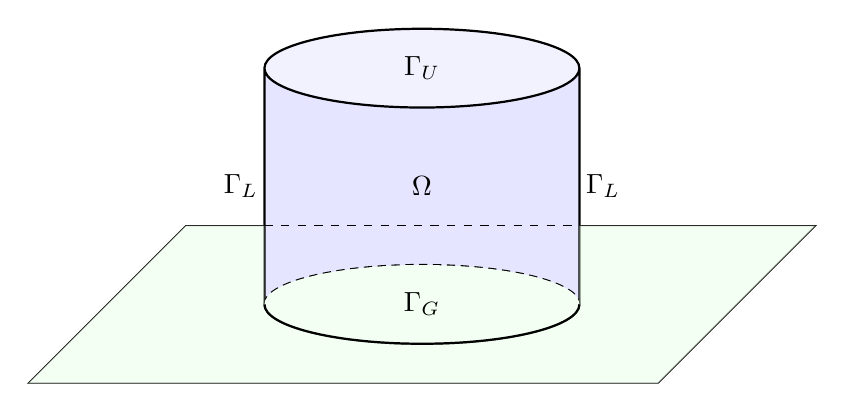
\begin{tikzpicture}
    \fill[color=blue!10] (2,0) -- (2,3) arc (360:180:2cm and 0.5cm) -- (-2,0) arc (180:360:2cm and 0.5cm);
    \fill[color=blue!5] (0,3) circle (2cm and 0.5cm);
    
    \draw[thick] (-2,3) -- (-2,0) arc (180:360:2cm and 0.5cm) -- (2,3) ++ (-2,0) circle (2cm and 0.5cm);
    \draw[densely dashed, thick] (-2,0) arc (180:0:2cm and 0.5cm);
    \draw (-2,1) -- (-3,1) --(-5,-1) -- (3,-1) -- (5,1) -- (2,1);
    \draw[dashed] (-2,1) -- (2,1);
    
    \fill[green!10,opacity=0.5] (-2,0) -- (-2,1) -- (-3,1) -- (-5,-1) -- (3,-1) -- (5,1) -- (2,1) -- (2,0) arc (0:180:2cm and -0.5cm);
    \fill[color=green!5] (0,0) circle (2cm and 0.5cm);
    
    \draw (0,1.5) node {$\Omega$};
    \draw (0,3) node {$\Gamma_U$};
    \draw (0,0) node {$\Gamma_G$};
    \draw (-2.3,1.5) node {$\Gamma_L$};
    \draw (2.3,1.5) node {$\Gamma_L$};
    
    \draw[thick] (2,0) arc (360:180:2cm and 0.5cm);
  \end{tikzpicture}
  \caption{The boundary structure of $\Omega$ for the case of weak solutions}
  \label{structdomaingraphboundaries_weak}
\end{figure}

The boundary conditions to describe the anisotropic system can be summarised as
  
    \begin{equation} \label{ANSC7-weak_coordinates_DWMC}
      \begin{split}
        & \mathbf{u}^\epsilon = 0 \text{ on } \Gamma \times (0,T), \\
        & c^\epsilon = 0 \text{ on } ( \Gamma_U \cup \Gamma_L) \times (0,T), \\
        & \partial_2 c^\epsilon = \partial_3 c^\epsilon = 0 \text{ on } \Gamma_G \times (0,T), \quad \partial_1 c^\epsilon = \sigma \in L^2 (0,T; \Gamma_G), \\
      \end{split}
    \end{equation}

while for the hydrostatic case we use
    
    \begin{equation} \label{HNSC7-weak_coordinates_DWMC}
      \begin{split} 
        & u_1 = u_2 = u_3 = 0 \text{ on } \Gamma \times (0,T) \\
        & c = 0 \text{ on } ( \Gamma_U \cup \Gamma_L) \times (0,T), \\
        & \partial_2 c = \partial_3 c = 0 \text{ on } \Gamma_G \times (0,T), \quad \partial_1 c = \sigma \in L^2 L^2 (0,T; \Gamma_G). \\
      \end{split}
    \end{equation}
    
The meaning of $\partial_1 c^\epsilon = \sigma$ above is that we naturally assume $\partial_1 c^\epsilon$ to be equal to some sufficiently regular $\sigma$ function defined on the respective boundary --- this well-known technique is also used for example for the case of modelling wind traction effect on the surface of the ocean (see \cite{azerad2001mathematical}).

As we have mentioned it in the introduction, in this case we will work with a more regular ${\mathbf{u}_h}_0 \in H^1$ initial data, so we directly use the $u_3 = 0$ equality on the boundary instead of the original $u_3 n_3 = 0$ constraint that we had used.
    
We highlight the difference between the boundary conditions of the original, east-north oriented, and the new, downwind-matching model for the case of weak solutions.

The difference in the kind of boundary conditions we can "afford" to have on the lower boundary for the concentration comes from the energy inequality. In the east-north-upwards oriented coordinate system we do not have an $\epsilon$ in the diffusion matrix, and thus, having any of the $\partial_i c^\epsilon$ terms different from 0 does not create any problems, not even for the case of the ocean where $\partial_3 c^\epsilon$ becomes nonzero as well (they are required however to be bounded of course). On the other hand, the downwind-matching coordinate system brings in an $\epsilon$ term in front of the $K_1$ diffusion coefficient, which makes the model more sensitive to assigning boundary conditions for $c^\epsilon.$ This means that we can not anymore have the relatively relaxed boundedness requirement for any $\partial_i c^\epsilon$ except for $i=1.$ All other $\partial_2 c^\epsilon, \partial_3 c^\epsilon$ derivatives must be zero on the lower boundary, otherwise they would result in an $(\epsilon - \text{const.})$ negative term appearing in the energy inequality --- for more details see Section $\ref{proof}$. This also means that we will consider exclusively the inland domain scenario for the case of this coordinate system.

Concerning the initial data, we set $${\mathbf{u}_h}_0 \in H^1 (\Omega), {u_3}_0 \in L^2(\Omega) \text{ with } \nabla \cdot \mathbf{u}_0 = 0, \text{ and } c_0 \in L^2 (\Omega).$$ We highlight here that we are still working in classical Leray framework of weak solutions, even though we use an $H^1(\Omega)$ regularity assumption on ${\mathbf{u}_h}_0,$ which is stronger than the more usual $L^2$ space regularity requirement for weak solutions (\cite{azerad2001mathematical}, \cite{pollatmws2019}). The reason we need this stronger regularity is to counterbalance the decreased control we have on the concentration function due to the coordinate choice, but overall this does not lead us out of the field of weak solutions.

Finally, the $s^\epsilon$ and $s$ source terms are formulated in the spirit of our previous result \cite{pollatmws2019}: the hydrostatic $s$ function is defined as a point source, while the anisotropic source function $s^\epsilon$ is modelled with a parametrised nascent delta function. For simplicity we assume here that the pollution process begins at $t = 0,$ thus we omit the multiplication by a Heaviside function representing the activation of the source, furthermore without loss of generality we assume that the source is centred in $x=0$ and we set the intensity constant $I$ to be $1.$

Let $\delta_\epsilon$ be the approximation of the $\delta$ distribution given below:

\begin{equation} \label{delta_eps_source_def}
\delta_\epsilon = 
  \begin{cases}
       \frac{1}{\epsilon^3} \exp{\bigg ( \frac{1}{\abs{{\frac{x}{\epsilon}}}^2-1} \bigg ) } &\quad \abs{x} < \epsilon \\
       0 &\quad \abs{x} \geq \epsilon. \\
  \end{cases}
\end{equation}

Following the main ideas described above, we set

\begin{equation}
  s^\epsilon = \delta_\epsilon, \quad s = \delta.
\end{equation}

%%% *** WEAK FORMULATION AND MAIN RESULT*** %%%
\subsection{Weak Formulation and Main Result} \label{weakformulationmainresult}

In this section we describe the weak formulation of the merged equations in both the anisotropic and hydrostatic case, and we state our main result.
  
  We need to define the following spaces:
  
  \[ C^{\infty}_\Gamma (\Omega) = \{ \varphi \in C^\infty (\bar{\Omega}); \varphi = 0 \text{ on some neighbourhood of } \Gamma\} \]
  
  \[ H^k_{\Gamma} (\Omega) = \overline{C_\Gamma ^ \infty (\Omega)} ^ {H^k (\Omega)} = \{ v \in H^k(\Omega); v=0 \text{ on } \Gamma \} \]
  
  \[ \mathbf{V} = \{ \mathbf{u} \in  H^1_{\Gamma} (\Omega) \times H^1_{\Gamma} (\Omega) \times H^1_{\Gamma} (\Omega); \nabla \cdot \mathbf{u} = 0 \text{ in } \Omega \} \]
  
  \[ H (\partial_3, \Omega) = \{ v \in L^2(\Omega); \partial_3 v \in L^2 (\Omega)\} \]
  
  \[ H_\Gamma (\partial_3, \Omega) = \overline{C_0 ^\infty (\Omega)}^{H (\partial_3, \Omega)} = \{ v \in H(\partial_3, \Omega); v = 0 \text{ on } \Gamma \} \]
  
  \[ \mathbf{W} = \{ \mathbf{u} \in  H^1_{\Gamma} (\Omega) \times H^1_{\Gamma} (\Omega) \times H_\Gamma (\partial_3, \Omega); \nabla \cdot \mathbf{u} = 0 \text{ in } \Omega \} \]
  
  Then the weak formulation of the hydrostatic system (\ref{HNSC1_coordinates_DWMC}) - (\ref{HNSC6_coordinates_DWMC}), (\ref{HNSC7-weak_coordinates_DWMC}) takes the following form.
  
  \begin{definition} \label{definitionhydrostaticWF}
  
  Find $(\mathbf{u}, c)$ such that $\mathbf{u} = (\mathbf{u}_h, u_3) \in L^2 (0, T; \mathbf{W})$ with $\mathbf{u}_h \in L^\infty (0,T; L^2(\Omega)^2),$ and $c \in L_t^\infty L_x^2$ with $\partial_2 c, \partial_3 c \in L^2_t L^2_x$, such that
  
  \begin{equation}
    \begin{split}
      & \int_0^T \bigg[ -(\mathbf{u}_h, \partial_t \mathbf{\tilde{u}}_h) + (\nabla_\nu \mathbf{u}_h, \nabla_\nu \mathbf{\tilde{u}}_h) - (\mathbf{u}_h, (\mathbf{u} \cdot \nabla) \mathbf{\tilde{u}}_h) + (b(\mathbf{u}_h), \mathbf{\tilde{u}}_h) \bigg ] \diff t \\
      & = - ({\mathbf{u}_h}_0, \mathbf{\tilde{u}}_h(0)) \diff t \label{hydrostaticWF}
    \end{split}
  \end{equation}
  
  and
  
  \begin{equation}
    \begin{split} \nonumber
      &+ \int_0^T \bigg[ -(c, \partial_t \tilde{c}) -(\mathbf{u}c, \nabla \tilde{c}) + K_2 (\partial_2 c, \partial_2 \tilde{c}) + K_3 (\partial_3 c, \partial_3 \tilde{c}) \bigg ] \diff t \\
      & = - (c_0, \tilde{c}(0)) + \int_0^T (s,\tilde{c}) \diff t
    \end{split}
  \end{equation}
  
  for all $(\mathbf{\tilde{u}}, \tilde{c})$ with $\mathbf{\tilde{u}} = (\mathbf{\tilde{u}}_h, \tilde{u}_3) \in H^1 (0,T, \mathbf{W})$, with $\mathbf{\tilde{u}}_h (T) = 0$ and $\partial_3 \mathbf{\tilde{u}}_h \in L^\infty (0, T; L^3 (\Omega)^2)$ and $\tilde{c}$ with $\tilde{c} \in L^2 (0,T, H^3_{\Gamma} (\Omega))$, $\tilde{c} \in H^1 (0,T, L^2)$, $\tilde{c} (T) = 0$. 
  
  \end{definition}
  
  Giving definition to the weak formulation of the (\ref{ANSC1_coordinates_DWMC}) - (\ref{ANSC6_coordinates_DWMC}), (\ref{ANSC7-weak_coordinates_DWMC}) anisotropic system we underline a feature regarding the spaces we use here. The velocity part of the solution is set to be in $C_w$ since it corresponds to the requirements of the proof detailed later. Even though we do not need the same weak continuity in time for the concentration function, this follows as a consequence once the velocity is a Leray-Hopf weak solution. Thus, overall we work with Leray-Hopf weak solutions, but the spaces in the below definition are kept minimal (in other words we use $L^\infty$ regularity instead of $C_w$ regularity where it is sufficient).

 \begin{definition} \label{definitionanisotropicWF}
  
  Find $\mathbf{u}^\epsilon = (\mathbf{u}_h, u^\epsilon_3) \in L^2 (0,T ; \mathbf{V}) \cap C_w (0, T; L^2 (\Omega)^3)$ and $c^\epsilon \in L^\infty (0,T; L^2(\Omega)) \cap L^2 (0,T; H^1(\Omega))$, such that
  
  \begin{equation}
    \begin{split}
      & \int_0^T \bigg [ -(\mathbf{u}^\epsilon_h, \partial_t \mathbf{\tilde{u}}_h) + (\nabla_\nu \mathbf{u}^\epsilon_h, \nabla_\nu \mathbf{\tilde{u}}_h) - (\mathbf{u}^\epsilon_h, (\mathbf{u}^\epsilon \cdot \nabla) \mathbf{\tilde{u}}_h) + (b(\mathbf{u}^\epsilon_h), \mathbf{\tilde{u}}_h) \bigg ] \diff t \\
      & + \epsilon \beta \int_0 ^ T \big [ (u_3 ^\epsilon, \tilde{u}_1) - (u_1^\epsilon, \tilde{u}_3) \big ] \diff t + \epsilon \alpha \int_0 ^ T \big [ (u_2 ^\epsilon, \tilde{u}_3) - (u_3^\epsilon, \tilde{u}_2) \big ] \diff t\\
      & + \epsilon^2 \int _0 ^ T \big [ -(u_3^\epsilon, \partial_t \tilde{u}_3) +(\mathbf{u}^\epsilon \cdot \nabla u_3 ^ \epsilon, \tilde{u}_3) + (\nabla_\nu u_3^\epsilon, \nabla_\nu \tilde{u}_3) \big ] \diff t \\
      & = - ({\mathbf{u}^\epsilon_h}_0, \mathbf{\tilde{u}}_h(0)) - \epsilon^2 ({u^\epsilon_3}_0, \tilde{u}_3 (0)) \diff t \raisetag{20pt} \label{anisotropicWF}
    \end{split}
  \end{equation}
  
    and
  
    \begin{equation}
    \begin{split} \nonumber
      & \int_0^T \bigg [ -(c^\epsilon, \partial_t \tilde{c}) -(\mathbf{u}^\epsilon c^\epsilon, \nabla \tilde{c}) + \epsilon K_1 (\partial_1 c^\epsilon, \partial_1 \tilde{c}) - \epsilon K_1 \sigma \big[\tilde{c} \big] _{\Gamma_G} \\
      & + K_2 (\partial_2 c^\epsilon, \partial_2 \tilde{c}) + K_3 (\partial_3 c^\epsilon, \partial_3 \tilde{c}) \bigg ] \diff t \\
      & =  - (c_0, \tilde{c} (0)) + \int_0^T (s^\epsilon,\tilde{c}) \diff t
    \end{split}
  \end{equation}
  
  for all $\mathbf{\tilde{u}} = (\mathbf{\tilde{u}}_h, \tilde{u}_3) \in H^1 (0,T;\mathbf{V})$ with $\mathbf{\tilde{u}}(T) = 0$ and $\tilde{c}$ such that $\tilde{c} \in H^1 (0,T, H^3_{\Gamma} (\Omega))$ and $\tilde{c} (T) = 0$.
  
  \end{definition}

Now we are ready to state the main theorem of this section.

\begin{theorem} \label{maintheoremWEAK}
  Let ${\mathbf{u}_h}_0$ $\in$ $H^1 (\Omega)$, ${u_3}_0 \in L^2(\Omega)$ with $\nabla \cdot \mathbf{u}_0 = 0, \mathbf{u}_0 = 0$ on $\partial \Omega$; let $c_0 \in$ $L^2 (\Omega)$, $c_0 = 0$ on $ \partial \Omega$, and assume that the boundary conditions (\ref{ANSC7-weak_coordinates_DWMC}) hold; then as the aspect ratio $\epsilon$ tends to zero, any weak solution $(\mathbf{u}^\epsilon, c^\epsilon)$ of the anisotropic equations (\ref{ANSC1_coordinates_DWMC}) - (\ref{ANSC6_coordinates_DWMC}) converges to a weak solution $(\mathbf{u}, c)$ of the hydrostatic equations of the polluted atmosphere (\ref{HNSC1_coordinates_DWMC}) - (\ref{HNSC6_coordinates_DWMC}).
\end{theorem}

The statement of the main theorem of this first part of the chapter is analogous to our previous result stated for the case of the geophysical frame, but we highlight the difference that here we use the initial data ${\mathbf{u}_h}_0 \in H^1,$ while for the case of the geophysical frame an $L^2$ initial velocity was sufficient.
  
%%% *** PROOF *** %%%
\subsection{Proof of the main theorem} \label{proof}

This section is dedicated to the verification of Theorem \ref{maintheoremWEAK}. Structurally we follow a similar chain of thought as in the previous chapter --- until the point where the proof diverges reaching the weak convergence of the nonlinear term $u_3^\epsilon c^\epsilon,$ where in this case we can not benefit from an $H^1$-regular concentration function. In more detail, we begin by calculating the energy inequality and collect the a priori estimates that derive from it, then verify the less problematic weak convergence results. Finally we elaborate the steps that bring the convergence of the $u_3^\epsilon c^\epsilon$ term to a closure. The main idea here is to temporarily ignore the $c^\epsilon$ function and prove a strong convergence result considering only the velocity functions. Throughout this step we go beyond the weak solutions quality and show that we are working with strong solutions. In this new setting with more favourable regularities we can prove the convergence result we need, and eventually return to the frame of weak solutions where we can merge back together the velocity and concentration functions into a unified solution. Finally as a byproduct we get a convergence rate for the velocity (see Proposition \ref{convrateweakframework}).

  \subsubsection{Energy inequality and a priori estimates}
  
  Calculating the energy inequality for the anisotropic system, we obtain that for a.e. $t \in [0,T]$ the following holds:
  
  \begin{equation}
    \begin{split}  
    & \frac{1}{2} (\norm{\mathbf{u}_h^\epsilon (t)}_{L^2}^2 + \epsilon ^ 2 \norm{u_3^\epsilon (t)}_{L^2}^2 + \norm{c^\epsilon (t)}_{L^2}^2) + \int_0 ^ t \big[ \norm{\nabla_\nu \mathbf{u}_h^\epsilon}_{L^2}^2 + \epsilon ^ 2 \norm{\nabla_\nu u_3^\epsilon}_{L^2}^2  \big] \diff \tau \\
    & + \int_0 ^ t  \big [ \epsilon K_1 \norm{\partial_1 c^\epsilon}_{L^2}^2  + K_2 \norm{\partial_2 c^\epsilon}_{L^2}^2 + K_3 \norm{\partial_3 c^\epsilon}_{L^2}^2 \big ] d \tau \\
    & \leq \int_0^t (s^\epsilon,c^\epsilon) \diff \tau + \frac{1}{2} (\norm{\mathbf{u}_h^\epsilon (0)}_{L^2}^2 + \epsilon ^ 2 \norm{u_3^\epsilon (0)}_{L^2}^2 + \norm{c^\epsilon_0}_{L^2}^2) \\
    & + \int _ 0 ^ t \epsilon K_1 \langle \partial_1 c^\epsilon, c^\epsilon \rangle_{\Gamma_G} \diff \tau \raisetag{70pt} \label{energyIEQ}
    \end{split}
  \end{equation}
  
  Using standard techniques, the generalised Young inequality with a $\zeta > 0$ constant, the H\"older inequality and the Trace Theorem, (\ref{energyIEQ}) takes the final form

  \begin{equation}
    \begin{split}  
    & \frac{1}{2} (\norm{\mathbf{u}_h^\epsilon (t)}_{L^2}^2 + \epsilon ^ 2 \norm{u_3^\epsilon (t)}_{L^2}^2 + \norm{c^\epsilon (t)}_{L^2}^2) + \int_0 ^ t \big [\norm{\nabla_\nu \mathbf{u}_h^\epsilon}_{L^2}^2 + \epsilon ^ 2 \norm{\nabla_\nu u_3^\epsilon}_{L^2}^2 \big ] \diff \tau \\
    & + \int_0 ^ t \bigg[ (\epsilon K_1 - \zeta \frac{\epsilon}{2} K_1 c_T (c_S + 1)) \norm{\partial_1 c^\epsilon}_{L^2}^2  + (K_2 - \zeta \frac{\epsilon}{2} K_1 c_T (c_S + 1)) \norm{\partial_2 c^\epsilon}_{L^2}^2 \\
    & + (K_3 - \zeta \frac{\epsilon}{2} K_1 c_T (c_S + 1)) \norm{\partial_3 c^\epsilon}_{L^2}^2 \bigg] \diff \tau \\
    & \leq \frac{1}{\zeta} K_1 \frac{\epsilon}{2} \int_0 ^ t \norm{\partial_1 c^\epsilon}^2 _{L^2 (\Gamma_G)} + \frac{1}{2} (\norm{\mathbf{u}_h^\epsilon (0)}_{L^2}^2 + \epsilon ^ 2 \norm{u_3^\epsilon (0)}_{L^2}^2 + \norm{c^\epsilon (0)}_{L^2}^2) \\
    & + \int_0^t (s^\epsilon, c^\epsilon) \diff \tau, \raisetag{20pt} \label{finalformEIEQ}
    \end{split}
  \end{equation}
  
  where $c_T$ and $c_S$ are the constants provided by the Trace Theorem and Sobolev embeddings. The boundary term is bounded because of the a priori assumptions made on the boundary conditions.
    
  The right-hand side of the energy inequality is now apparently bounded, and it is easy to see that the coefficients of the pollution terms on the left-hand side are positive, since the $\zeta$ constant of the generalised Young inequality can be freely chosen in a way such that the requirements $\epsilon K_1 (1 - \zeta \frac{1}{2} c_T (c_S + 1)) > 0, (K_2 - \zeta \frac{\epsilon}{2} K_1 c_T (c_S + 1)) > 0, (K_3 - \zeta \frac{\epsilon}{2} K_1 c_T (c_S + 1)) > 0 $ are all satisfied.
  
  We note that the most significant difference in this new form of the energy inequality (\ref{finalformEIEQ}) is having $\sqrt{\epsilon} \partial_1 c^\epsilon$ in the place of $\partial_1 c^\epsilon,$ which is what we had for the case of the geophysical coordinate system. It leads to the disappearance of the $H^1$ regularity of $c^\epsilon,$ and thus we don't have the strong convergence feature of the concentration function anymore --- which was of key importance for proving the weak convergence of a nonlinear term in the case of the classical geophysical frame.
  
  This form of the energy inequality also shows why we need the $\partial_2 c^\epsilon, \partial_3 c^\epsilon$ terms to vanish on the boundary. Otherwise, using the Trace Theorem on these boundary terms would contribute to the appearance of negative, $\epsilon$-free terms in the coefficient of $\norm{\partial_1 c^\epsilon}_{L^2}^2,$ which would undermine the structure of the energy inequality.
  
  From the final form of the energy inequality (\ref{finalformEIEQ}) we obtain uniform a priori estimates that we summarise in the following proposition.
  
  \begin{prop} \label{aprioriprop}
    Let $u^\epsilon_1, u^\epsilon_2, u^\epsilon_3$ and $c^\epsilon$ be the weak solutions of the system (\ref{ANSC1_coordinates_DWMC}) - (\ref{ANSC5_coordinates_DWMC}) in the sense of Definition \ref{definitionanisotropicWF}. Then it holds,
    
    \begin{align}
      & u^\epsilon_1, u^\epsilon_2, \epsilon u^\epsilon_3, c^\epsilon & \quad & \text{are bounded in $L^\infty (0,T; L^2(\Omega)),$} \label{proposition1} \\
      & u^\epsilon_3 & \quad & \text{is bounded in $L^2 (0,T; L^2(\Omega)),$} \label{propositionExtra} \\
      & u^\epsilon_1, u^\epsilon_2, \epsilon u^\epsilon_3 & \quad & \text{are bounded in $L^2(0,T; H^1(\Omega)),$} \label{proposition2} \\
      & \sqrt{\epsilon} \partial_1 c^\epsilon, \partial_2 c^\epsilon, \partial_3 c^\epsilon & \quad & \text{are bounded in $L^2(0,T;L^2(\Omega)).$} \label{proposition3}
    \end{align}
    
  \end{prop}
  
  For the details of the proof see \cite{pollatmws2019}.
  
    \subsubsection{Weak convergence - Part 1.}
  
  The convergence of the linear terms and also the convergence of the nonlinear terms with the exception of $u_3^\epsilon c^\epsilon$ can be proved analogously as in the previous chapter --- the proofs of these properties are not affected by the changes induced by choosing to use the downwind-matching coordinate system. Hence, for completeness we will describe the main steps leading up to obtaining these results, but we will skip the details. For technical or specific issues see \cite{azerad2001mathematical} and \cite{pollatmws2019}.
  
  As a consequence of Proposition \ref{aprioriprop}, up to subsequences still denoted by the same way, we have the following weak convergence results.
  
    \begin{align} 
    &  \mathbf{u}_h^\epsilon \rightharpoonup \mathbf{u}_h &\quad & \text{weakly in $L_t^\infty L_x^2 \cap L_t^2 H_x^1$,} \label{WeakConvUHEps} \\
    &  \epsilon^2 u_3^\epsilon \to 0 &\quad & \text{strongly in $L_t^\infty L_x^2 \cap L_t^2 H_x^1$,} \label{WeakConvU3Eps} \\ 
    & u_3^\epsilon \rightharpoonup u_3  &\quad & \text{weakly in $L_t^2 L_x^2$,} \label{WeakConvU3NoEps} \\
    & c^\epsilon \rightharpoonup c &\quad & \text{weakly in $L_t^\infty L_x^2$,} \label{WeakConvCEps1} \\
    & \partial_2 c^\epsilon \rightharpoonup \partial_2 c &\quad & \text{weakly in $L_t^2 L_x^2$,} \label{WeakConvCEps2} \\
    & \partial_3 c^\epsilon \rightharpoonup \partial_3 c &\quad & \text{weakly in $L_t^2 L_x^2$,} \label{WeakConvCEps3} \\
    & \sqrt{\epsilon} \partial_1 c^\epsilon \rightharpoonup e &\quad & \text{weakly for some limit element $e$ in $L_t^2 L_x^2$.} \label{WeakConvCEps4}
  \end{align} 
  
  In order to conclude the proof of Theorem \ref{maintheoremWEAK} we pass to the limit in the weak formulation (\ref{anisotropicWF}). Taking the limit for the linear terms can be done in a standard way using the previously obtained results.
   Concerning the nonlinear velocity terms (i.e. nonlinear terms that do not include the concentration function), the convergence can be shown applying a generalisation of the classical translation criterium of Riesz-Frechet-Kolmogorov which enables us to get strong convergence for the horizontal velocities. This is achieved by establishing a bound for the perturbation of $\mathbf{u}_h$ of the form $\norm{\tau_\pi \mathbf{u}_h - \mathbf{u}_h}_{L^2(0,T-\pi, {H^2}^*)} \leq \lambda(\pi) + \mu(\epsilon),$ where $\lambda$ and $\mu$ are appropriate functions with their limits vanishing at zero, and $\tau_\pi \mathbf{u}_h = \mathbf{u}_h (t+\pi) $. After obtaining strong convergence for $\mathbf{u}_h,$ the proof of the convergence for these nonlinear terms can be closed by applying basic interpolation techniques and the generalised H\"older inequality. 
  Finally, as for the concentration-including nonlinear terms, we have the convergence of $(u_i c^\epsilon, \partial_i \tilde{c})$ for $i=1,2,$ since as we mentioned before, we have the strong convergence of the horizontal velocities --- while in the case of $i=3$ this property does not hold for $u_3$ and from the energy bound we do not have more than the weak convergence of $c^\epsilon$. Because of its complexity we handle this specific nonlinear compound product term in the next section.
  
  \subsubsection{Weak convergence - Part 2.}
  
  As we mentioned before, the cornerstone idea for obtaining the convergence of the remaining product term $u_3^\epsilon c^\epsilon$ is to exploit the $H^1$ regularity of the initial horizontal velocity. Indeed, given an $H^1$ initial data for $\mathbf{u}_h,$ according to the theory developed in \cite{cao2007global}, there exists a unique global strong solution for the primitive equations $(\ref{HNSC1_coordinates_DWMC})$ - $(\ref{HNSC4_coordinates_DWMC}).$ We recall here this result (for more details see \cite{cao2007global}).
  
  \begin{theorem} \label{PE3DWellPosedness}
    Let ${\mathbf{u}_h}_0 \in H^1(\Omega).$ Then there exists a unique strong solution $\mathbf{u}_h$ of the reformulated Primitive Equations $(\ref{HNSC1_coordinates_DWMC})$ - $(\ref{HNSC4_coordinates_DWMC})$, $(\ref{HNSC6_coordinates_DWMC})$ such that $$\mathbf{u}_h \in C([0, \infty), H^1(\Omega)) \cap L^2_{loc}([0, \infty), H^2(\Omega))$$ and $$\partial_t \mathbf{u}_h \in L^2_{loc} ([0,\infty), L^2(\Omega)).$$
  \end{theorem}
  
  In more detail, we have the following regularities for the strong solution of the primitive equations for the case of an $H^1$ initial data:
  
  \begin{corollary} \label{StrongSolPE_boundedness}
  
    Let $(\mathbf{u}_h,u_3)$ be the the unique global strong solution to the primitive equations (\ref{HNSC1_coordinates_DWMC}) - (\ref{HNSC4_coordinates_DWMC}) with an initial data ${\mathbf{u}_h}_0 \in H^1(\Omega).$ Then we have the following boundedness result:
    
    $$ \sup_{0 \leq t < \infty} \norm{\mathbf{u}_h}_{H^1}^2 (t) + \int_0^\infty \norm{\nabla \mathbf{u}_h}_{H^1}^2 \diff t \leq \kappa (\norm{{\mathbf{u}_h}_0}_{H^1}, \Gamma_G).$$
  
  \end{corollary}
  
  This is a direct consequence of Theorem \ref{PE3DWellPosedness}, but for completeness we also mention that for the simpler case of a periodic domain it has also been verified in \cite{li2019primitive}, where the proof becomes more straightforward thanks to the structure of the domain.
  
  The result of Corollary \ref{StrongSolPE_boundedness} on the strong solutions of the primitive equations will be indispensable later, as we will use these strong solution functions for testing the scaled Navier-Stokes equations.
  
  The following part of the proof is dedicated to verifying the strong convergence of $u_3^\epsilon,$ and is based on the idea of \cite{li2019primitive} --- our scenario is different however in that \textit{a)} first of all our domain is bounded, while the domain the authors of \cite{li2019primitive} consider is periodic, \textit{b)} we do not assume zero-averaged functions, and finally \textit{c)} in our case the Coriolis terms are incorporated to the model as well. Our strategy in providing the proof is to give a self-contained result that describes all the steps that build up the verification process, but we elaborate in more detail where the above mentioned \textit{a), b), c)} points have a tangible effect. Some technical details that are identical to those in \cite{li2019primitive} will be skipped.

Another structural difference we need to underline in connection with the proof is that instead of using the $[-1,1]$ set to represent the $\epsilon$-free vertical domain (i.e. the $\Gamma_L$ section), we use $[0,1],$ without assuming the vertical velocity function $u_3^\epsilon$ to be odd with respect to $z.$ The vertical section is commonly set to $[-1,1],$ or equivalently, to $[-a,a]$ in works that use the periodical domain scenario, see also \cite{cao2016global}, \cite{cao2017global}. In our case however we use a bounded domain without the assuming a symmetry line in the vertical midpoint --- thus we work with the $[0,1]$ set as the vertical domain. As a consequence, the Ladyzhenskaya-type inequality presented in different versions in \cite{cao2003global} and \cite{li2019primitive} will be used here in the following form:

\begin{lemma}\label{LadyzhenskayatypeIEQ}

  The inequalities
  
  \begin{equation}\nonumber
    \begin{split}
      & \int_{\Gamma_G} \bigg ( \int_0^1 f(x,y,z) \diff z \bigg) \bigg ( \int_0^1 g(x,y,z) h(x,y,z) \diff z \bigg ) \diff x \diff y \\
      & \lesssim \norm{f}_2^{1/2} \big ( \norm{f}_2^{1/2} + \norm{\nabla_h f}_2^{1/2} \big ) \norm{g}_2 \norm{h}_2^{1/2} \big (\norm{h}_2^{1/2} + \norm{\nabla_h h}_2^{1/2} \big ),
    \end{split}
  \end{equation}
  
  and
  
  \begin{equation}\nonumber
    \begin{split}
      & \int_{\Gamma_G} \bigg ( \int_0^1 f(x,y,z) \diff z \bigg) \bigg ( \int_0^1 g(x,y,z) h(x,y,z) \diff z \bigg ) \diff x \diff y \\
      & \lesssim \norm{f}_2 \norm{g}_2^{1/2} \big ( \norm{g}_2^{1/2} + \norm{\nabla_h g}_2^{1/2} \big ) \norm{h}_2^{1/2} \big (\norm{h}_2^{1/2} + \norm{\nabla_h h}_2^{1/2} \big )
    \end{split}
  \end{equation}
  
  hold true for any $f,g,h$ set of functions such that the right-hand sides make sense and are finite.

\end{lemma}

Note that this lemma simply states the inequality for the complete domain even in the version in \cite{li2019primitive}, not assuming an odd $u_3^\epsilon$ function or a $z$-symmetrical vertical structure of $\Omega$.
  
The main idea in order to prove the strong convergence of $u^\epsilon_3$ lies in establishing a bound of $O(\epsilon^a)$ for some $a>0$ for the difference \begin{equation}\label{velocitydifferencefunctions}(\mathbf{U}_h^\epsilon, U_3^\epsilon): = (\mathbf{u}_h^\epsilon - \mathbf{u}_h, u_3^\epsilon - u_3).\end{equation} This will be achieved by using the strong solution $(\mathbf{u}_h,u_3)$ as a test function in the weak formulation's integral identity $(\ref{anisotropicWF})$. Following this method we arrive to

\begin{prop} \label{propIdentity}

Let $(\mathbf{u}_h^\epsilon, u_3^\epsilon)$ and $(\mathbf{u}_h,u_3)$ be the solutions of (\ref{ANSC1_coordinates_DWMC}) - (\ref{ANSC4_coordinates_DWMC}) and (\ref{HNSC1_coordinates_DWMC}) - (\ref{HNSC4_coordinates_DWMC}), respectively, with initial data $({\mathbf{u}_h}_0, {u_3}_0),$ where ${\mathbf{u}_h}_0 \in H^1(\Omega)$ and ${u_3}_0 = - \int_0^z \nabla_h \cdot {\mathbf{u}_h}_0 \diff z'.$ Then we have the following integral identity:

\begin{equation} \label{integralIdentity_prop}
  \begin{split}
    & - \frac{\epsilon^2}{2} \norm{u_3(t)}_2^2 + \bigg ( (\mathbf{u}_h^\epsilon \cdot \mathbf{u}_h + \epsilon^2 u_3^\epsilon u_3) \diff x \diff y \diff z  \bigg ) (t) \\
    & + \int_{Q_t} (-\mathbf{u}_h^\epsilon \cdot \partial_t \mathbf{u}_h + \nabla \mathbf{u}_h^\epsilon : \nabla \mathbf{u}_h + \epsilon^2 \nabla u_3^\epsilon \cdot \nabla u_3) \diff x \diff y \diff z \diff s \\
    & = \frac{\epsilon^2}{2} \norm{{u_3}_0}_2^2 + \norm{{\mathbf{u}_h}_0}_2^2 + \epsilon^2 \int_{Q_t} \bigg ( \int_0^z \partial_t \mathbf{u}_h \diff z' \bigg ) \cdot \nabla_h U_3^\epsilon \diff x \diff y \diff z \diff s \\
    & - \int_{Q_t} [(\mathbf{u}^\epsilon \cdot \nabla) \mathbf{u}_h^\epsilon \cdot \mathbf{u}_h + \epsilon^2 \mathbf{u}^\epsilon \cdot \nabla u_3^\epsilon u_3] \diff x \diff y \diff z \diff s \\
    & + \int_{Q_t}  ( \gamma u_2^\epsilon u_1 - \epsilon \beta u_3^\epsilon u_1 + \alpha \epsilon u_3^\epsilon u_2 - \gamma u_1^\epsilon u_2 - \epsilon \alpha u^\epsilon_2 u_3 + \epsilon \beta u_1^\epsilon u_3)
  \end{split}
\end{equation}

for any $t \in [0, \infty),$ where $Q_t = \Omega \times (0,t).$

\end{prop}

\begin{proof}

We recall the definition of weak solution for the scaled Navier-Stokes equations:

\begin{equation} \label{WFreminder}
  \begin{split}
    & \int_Q [ - (\mathbf{u}_h^\epsilon \cdot \partial_t \tilde{\mathbf{u}}_h + \epsilon^2 u_3^\epsilon \partial_t \tilde{u}_3) +( (\mathbf{u}^\epsilon \cdot \nabla) \mathbf{u}_h^\epsilon \cdot \tilde{\mathbf{u}}_h + \epsilon^2 \mathbf{u}^\epsilon \cdot \nabla u_3^\epsilon \tilde{u}_3 ) + \nabla \mathbf{u}_h^\epsilon : \nabla \tilde{\mathbf{u}}_h \\
    & + \epsilon^2 \nabla u_3^\epsilon \cdot \nabla \tilde{u}_3 ] \diff x \diff y \diff z \diff t = \int_Q ({\mathbf{u}_h}_0 \cdot \tilde{\mathbf{u}}_h (\cdot , 0) + \epsilon^2 {u_3}_0 \tilde{u}_3 (\cdot , 0)) \diff x \diff y \diff z \\
    & + \int_Q  \gamma u_2^\epsilon \tilde{u}_1 - \epsilon \beta u_3^\epsilon \tilde{u}_1 + \alpha \epsilon u_3^\epsilon \tilde{u}_2 - \gamma u_1^\epsilon \tilde{u}_2 - \epsilon \alpha u_2^\epsilon \tilde{u}_3 + \epsilon \beta u_1^\epsilon \tilde{u}_3
  \end{split}
\end{equation}

for any $\tilde{\mathbf{u}} = (\tilde{\mathbf{u}}_h, \tilde{u}_3) \in H^1 (0,T;\mathbf{V})$ with $\tilde{\mathbf{u}}(T) = 0.$

Now, let's define $\chi \in C_0^\infty ([0, \infty))$ with $0 \leq \chi \leq 1$ and $\chi (0) = 1$ and set $\tilde{\mathbf{u}} = (\mathbf{u}_h,u_3) \chi (t).$ By using the density argument it is valid to choose this $\tilde{\mathbf{u}}$ function as a testing function as long as all the integral terms remain well-defined in $(\ref{WFreminder}),$ which we verify in the following.

It is important to highlight at this point that since we are not restricted to zero-averaged functions and we are not on a periodic domain, we need to pay special attention when verifying boundedness results using the Poincar\'e inequality. Note that as the value of the velocity functions are defined to be zero on the boundary, any first-order estimate of the type $\norm{\mathbf{u}_h^\epsilon} \leq \norm{\nabla \mathbf{u}_h^\epsilon}$ is valid, using the zero-trace version of the Poincar\'e inequality for functions in $W^{1,2}_0.$ However, since it is only the value of the functions that vanishes on the boundary, but not their derivatives, higher order estimates such as passing from $\norm{\nabla \mathbf{u}_h^\epsilon}$ to $\norm{\Delta \mathbf{u}_h^\epsilon}$ in the process of constructing an upper bound can not be applied in general. Which is why, for example, the estimate of the the term below is rather involved as follows:

\begin{equation}
  \begin{split}
    & \int_Q \abs{\mathbf{u}^\epsilon} \abs{\nabla u_3^\epsilon} \abs{u_3} \chi \diff x \diff y \diff z \\
    & \leq  \int_0 ^ T \int_{\Gamma_G} \bigg ( \int_0^1 \abs{\mathbf{u}^\epsilon} \abs{\nabla u_3^\epsilon} \diff z \int_0^1 \abs{\nabla_h \mathbf{u}_h} \diff z \bigg ) \diff x \diff y \diff t \\
    & \lesssim \int_0^T \norm{\mathbf{u}^\epsilon}_2^{1/2} \norm{\nabla \mathbf{u}^\epsilon}_2^{1/2} \norm{\nabla u_3^\epsilon}_2 \norm{\nabla_h \mathbf{u}_h}_2^{1/2} (\norm{\nabla_h \mathbf{u}_h}_2^{1/2} + \norm{\Delta \mathbf{u}_h}_2^{1/2}) \diff t \\
    & \lesssim \sup_{0 \leq t \leq T} \bigg( \norm{\mathbf{u}^\epsilon}_2^{1/2} \norm{\nabla \mathbf{u}_h}_2^{1/2} \bigg) \bigg( \int_0^T \norm{\nabla \mathbf{u}^\epsilon}^2_2 \diff t \bigg)^{1/4} \bigg ( \int_0^T \norm{\nabla u_3^\epsilon}_2^2 \diff t \bigg)^{1/2} \\
    & \times \bigg ( \int_0^T \norm{\Delta \mathbf{u}_h}_2^2 \diff t \bigg )^{1/4} \\
    & + \sup_{0 \leq t \leq T} \bigg( \norm{\mathbf{u}^\epsilon}_2^{1/2} \norm{\nabla \mathbf{u}_h}_2 \bigg) \bigg( \int_0^T \norm{\nabla \mathbf{u}^\epsilon}_2 \diff t \bigg)^{1/2} \bigg ( \int_0^T \norm{\nabla u_3^\epsilon}_2^2 \diff t \bigg)^{1/2}.\raisetag{60pt}
  \end{split}
\end{equation}

The validity of the remaining integral terms are not affected by the boundary change and they are guaranteed by the regularities of the respective solution functions and using basic inequalities. For completeness we remark that the more delicate and problematic terms -- i.e. the terms where the testing function is defined via the less regular $u_3$ vertical velocity -- are still well-defined. This can be verified firstly by rewriting the $\int_Q u^\epsilon_3 \partial_t \tilde{u}_3$ term as

$$ \int_Q u^\epsilon_3 \partial_t (u_3 \chi) \diff x \diff y \diff z \diff t = \int_0^\infty \langle \partial_t (u_3 \chi), u^\epsilon_3 \rangle _ {H^{-1} \times H^1} \diff t.$$

The validity of the integral term can be shown using this modified form pointing out that $\partial_t \mathbf{u}_h$ is in $L^2_{loc} ([0,\infty), L^2(\Omega))$ because of Theorem $\ref{PE3DWellPosedness}$, and as a consequence $\partial_t u_3$ has an $H^{-1}$ space regularity (using the divergence-free condition).

On the other hand, the $ \int_Q \nabla u^\epsilon_3 : \nabla (u_3 \chi) $ term is well-defined since $u_3$ as a strong solution has $H^1$ space regularity, and the same holds for the weak solution $u^\epsilon_3.$

Now we are justified to take $\tilde{\mathbf{u}}$ as a test function, and thus, rewriting some of the integral terms in $(\ref{WFreminder})$ in a more convenient form, we have

\begin{equation} \label{rewrittenform}
  \begin{split}
    & \int_Q (- \mathbf{u}_h^\epsilon \cdot \partial_t \mathbf{u}_h + \nabla \mathbf{u}_h^\epsilon : \nabla \mathbf{u}_h + \epsilon^2 \nabla u_3^\epsilon \cdot \nabla u_3) \chi \diff x \diff y \diff z \diff t \\
    & - \epsilon^2 \int_0^\infty \langle \partial_t u_3 , u_3^\epsilon \rangle _{H^{-1} \times H^1} \chi \diff t - \int_Q (\mathbf{u}_h^\epsilon \cdot \mathbf{u}_h + \epsilon^2 u_3^\epsilon u_3) \chi' \diff x \diff y \diff z \diff t \\
    & = - \int_Q [(\mathbf{u}^\epsilon \cdot \nabla) \mathbf{u}_h^\epsilon \cdot \mathbf{u}_h + \epsilon^2 \mathbf{u}^\epsilon \cdot \nabla u_3^\epsilon u_3] \chi \diff x \diff y \diff z \diff t + \norm{{\mathbf{u}_h}_0}_2^2 + \epsilon^2 \norm{{u_3}_0}_2^2 \\
    & + \int_Q  ( \gamma u_2^\epsilon u_1 - \epsilon \beta u_3^\epsilon u_1 + \alpha \epsilon u_3^\epsilon u_2 - \gamma u_1^\epsilon u_2 - \epsilon \alpha u^\epsilon_2 u_3 + \epsilon \beta u_1^\epsilon u_3) \chi,\raisetag{80pt}
  \end{split}
\end{equation}

for any $\chi \in C^\infty_0 ([0,\infty)),$ with $0 \leq \chi \leq 1$ and $\chi (0) = 1.$

Since the estimate $(\ref{integralIdentity_prop})$ is localised in time, we take an arbitrary $t_0 \in (0, \infty)$ and a sufficiently small positive $\delta \in (0, t_0).$ Choose a cut-off function with the properties $\chi_\delta \in C^\infty_0 [0,t_0),$ such that $\chi_\delta \equiv 1$ on $[0, t_0 -\delta], 0 \leq \chi_\delta \leq 1$ on $[t_0 - \delta, t_0 )$ and $\abs{\chi_\delta '} \leq \frac{2}{\delta}$ on $[0, t_0).$ Now, taking $\chi = \chi_\delta$ in $(\ref{rewrittenform})$ as $\delta \to 0,$ one can arrive to the desired equality after performing the calculations for passing to the limit. It is easy to see that because of the velocities vanishing on the boundaries, the technical details remain uneffected, even though we are not on a periodic domain.

In more detail, the term $ \langle \partial_t u_3, u_3^\epsilon \rangle _{H^{-1} \times H^1}$ now takes the form 

\begin{equation}
  \begin{split}
    & \langle \partial_t u_3, u_3^\epsilon \rangle _{H^{-1} \times H^1} = - \bigg \langle \nabla_h \cdot \bigg ( \int_0^z \partial_t \mathbf{u}_h \diff z' \bigg ) , u_3^\epsilon \bigg \rangle \\
    & = - \int_{\partial \Omega} \bigg ( \int_0^z \partial_t \mathbf{u}_h \diff z' \bigg ) u_3^\epsilon \mathbf{n}_h + \int_\Omega \bigg ( \int_0^z \partial_t \mathbf{u}_h \diff z' \bigg) \cdot \nabla_h u_3^\epsilon \diff x \diff y \diff z,
  \end{split}
\end{equation}

where $\mathbf{n}_h$ is the horizontal component of the outward facing normal vector on the $\partial \Omega$ boundary.
    
By using that $u_3^\epsilon = 0$ on $\partial \Omega$ we arrive easily to the more simple
    
$$ \langle \partial_t u_3, u_3^\epsilon \rangle _{H^{-1} \times H^1} = \int_\Omega \bigg ( \int_0^z \partial_t \mathbf{u}_h \diff z' \bigg) \cdot \nabla_h u_3^\epsilon \diff x \diff y \diff z,$$
     
which is the form one would have on a periodic domain. Similarly, 
     
$$ \langle \partial_t u_3, u_3^\epsilon - u_3 \rangle _{H^{-1} \times H^1} = \int_\Omega \bigg ( \int_0^z \partial_t \mathbf{u}_h \diff z' \bigg) \cdot \nabla_h (u_3^\epsilon - u_3),$$ as the boundary term $$\int_{\partial \Omega} \bigg ( \int_0^z \partial_t \mathbf{u}_h \diff z' \bigg ) (u_3^\epsilon - u_3) \mathbf{n}_h$$ becomes zero, since we have $u_3 = 0, u_3^\epsilon = 0$ on $\Gamma.$ 

After some technical details that we omit here we eventually obtain

\begin{equation}
  \begin{split}
    & - \frac{\epsilon^2}{2} \norm{u_3(t_0)}_2^2 + \bigg ( (\mathbf{u}_h^\epsilon \cdot \mathbf{u}_h + \epsilon^2 u_3^\epsilon u_3) \diff x \diff y \diff z  \bigg ) (t_0) \\
    & + \int_{Q_{t_0}} (-\mathbf{u}_h^\epsilon \cdot \partial_t \mathbf{u}_h + \nabla \mathbf{u}_h^\epsilon : \nabla \mathbf{u}_h + \epsilon^2 \nabla u_3^\epsilon \cdot \nabla u_3) \diff x \diff y \diff z \diff t \\
    & = \frac{\epsilon^2}{2} \norm{{u_3}_0}_2^2 + \norm{{\mathbf{u}_h}_0}_2^2 + \epsilon^2 \int_{Q_{t_0}} \bigg ( \int_0^z \partial_t \mathbf{u}_h \diff z' \bigg ) \cdot \nabla_h U_3^\epsilon \diff x \diff y \diff z \diff t \\
    & - \int_{Q_{t_0}} [(\mathbf{u}^\epsilon \cdot \nabla) \mathbf{u}_h^\epsilon \cdot \mathbf{u}_h + \epsilon^2 \mathbf{u}^\epsilon \cdot \nabla u_3^\epsilon u_3] \diff x \diff y \diff z \diff t \\
    & + \int_{Q_{t_0}}  ( \gamma u_2^\epsilon u_1 - \epsilon \beta u_3^\epsilon u_1 + \alpha \epsilon u_3^\epsilon u_2 - \gamma u_1^\epsilon u_2 - \epsilon \alpha u_2^\epsilon u_3 + \epsilon \beta u_1^\epsilon u_3)
  \end{split}
\end{equation}

for any $t_0 \in [0, \infty),$ which verifies the statement of the proposition.

\end{proof}

With this we are ready to estimate the difference between the solutions of the scaled and hydrostatic equations, which is described by the following proposition.

\begin{prop} \label{convrateweakframework}

Let $(\mathbf{u}_h^\epsilon, u_3^\epsilon)$ and $(\mathbf{u}_h,u_3)$ be the solutions of (\ref{ANSC1_coordinates_DWMC}) - (\ref{ANSC4_coordinates_DWMC}) and (\ref{HNSC1_coordinates_DWMC}) - (\ref{HNSC4_coordinates_DWMC}), respectively, with initial data $({\mathbf{u}_h}_0, {u_3}_0),$ where ${\mathbf{u}_h}_0 \in H^1(\Omega)$ and ${u_3}_0 = - \int_0^z \nabla_h \cdot {\mathbf{u}_h}_0 \diff z'.$ Then the following estimate holds for the difference function $(\mathbf{U}_h^\epsilon, U_3^\epsilon):$

\begin{equation}
  \begin{split}
    & \sup_{0 \leq t < \infty} ( \norm{\mathbf{U}_h^\epsilon}_2^2 + \epsilon^2 \norm{U_3^\epsilon}_2^2)(t) + \int_0 ^ \infty ( \norm{\nabla \mathbf{U}_h^\epsilon}_2^2 + \epsilon^2 \norm{\nabla U_3^\epsilon}_2^2)\diff s \\
    & \leq \kappa (\norm{{\mathbf{u}_h}_0}_{H^1}, \Gamma_G) \epsilon^2 (\norm{{\mathbf{u}_h}_0}_2^2 + \epsilon^2 \norm{{u_3}_0}_2^2 + 1).
  \end{split}
\end{equation}

\end{prop}

\begin{proof}

  Multiplying the horizontal part of the hydrostatic equations, i.e. equations ($\ref{HNSC1_coordinates_DWMC}$)--($\ref{HNSC2_coordinates_DWMC}$) by $\mathbf{u}_h^\epsilon$ and integrating the result over $Q_{t_0},$ by utilising the divergence-free condition and the zero velocity boundary conditions, we have
  
  \begin{equation} \label{identity_obtained_by_v_eps}
    \begin{split}
      & \int_{Q_{t_0}} (\partial_t \mathbf{u}_h \cdot \mathbf{u}_h^\epsilon + \nabla \mathbf{u}_h : \nabla \mathbf{u}_h^\epsilon) \diff x \diff y \diff z \diff t \\
      & = - \int_{Q_{t_0}} (\mathbf{u} \cdot \nabla) \mathbf{u}_h \cdot \mathbf{u}_h^\epsilon + \gamma u_2 u_1^\epsilon - \gamma u_1 u_2^\epsilon \diff x \diff y \diff z \diff t.
    \end{split}
  \end{equation}
  
  On the other hand, multiplying the same ($\ref{HNSC1_coordinates_DWMC}$)--($\ref{HNSC2_coordinates_DWMC}$) equations by $\mathbf{u}_h$ instead, and integrating again on $Q_{t_0},$ we arrive to
  
  \begin{equation} \label{identity_obtained_by_v}
    \frac{1}{2} \norm{\mathbf{u}_h(t_0)}_2^2 + \int_0^{t_0} \norm{\nabla \mathbf{u}_h}_2^2 \diff t = \frac{1}{2} \norm{{\mathbf{u}_h}_0}_2^2,
  \end{equation}
  
  for any $t_0 \in [0, \infty).$ At the same time we also know by definition that
  
  \begin{equation} \label{bound_by_definition}
    \begin{split}
      & \frac{1}{2}( \norm{\mathbf{u}_h^\epsilon (t_0)}_2^2 + \epsilon^2 \norm{u_3^\epsilon(t_0)}_2^2)+ \int_0^{t_0} (\norm{\nabla \mathbf{u}_h^\epsilon}_2^2 + \epsilon^2 \norm{\nabla u_3^\epsilon}_2^2) \diff s \\
      & \leq \frac{1}{2} (\norm{{\mathbf{u}_h}_0}_2^2 + \epsilon^2 \norm{{u_3}_0}_2^2),
    \end{split}
  \end{equation}
  
  for almost every $t_0 \in [0, \infty).$
  
  Now, summing ($\ref{bound_by_definition}$) and ($\ref{identity_obtained_by_v}$) and from their result subtracting ($\ref{integralIdentity_prop}$) (where we take $t= t_0$) and ($\ref{identity_obtained_by_v_eps}$) we obtain
  
  \begin{equation} \label{introduce_I_terms}
    \begin{split}
      & \frac{1}{2} (\norm{\mathbf{U}_h^\epsilon}_2^2 + \epsilon^2 \norm{U_3^\epsilon}_2^2) (t_0) + \int_0^{t_0} (\norm{\nabla \mathbf{U}_h^\epsilon}_2^2 + \epsilon^2 \norm{\nabla U_3^\epsilon}_2^2) \diff t  \\
      & \leq - \epsilon^2 \int_{Q_{t_0}} \bigg [ \bigg ( \int_0^z \partial_t \mathbf{u}_h \diff z' \bigg ) \cdot \nabla_h U_3^\epsilon + \nabla u_3 \cdot \nabla U_3^\epsilon \bigg ] \diff x \diff y \diff z \diff t \\
      & + \int_{Q_{t_0}} [(\mathbf{u}^\epsilon \cdot \nabla) \mathbf{u}_h^\epsilon \cdot \mathbf{u}_h + (\mathbf{u} \cdot \nabla )\mathbf{u}_h \cdot \mathbf{u}_h^\epsilon] \diff x \diff y \diff z \diff t \\
      & + \epsilon^2 \int_{Q_{t_0}} \mathbf{u}^\epsilon \cdot \nabla u_3^\epsilon u_3 \diff x \diff y \diff z \diff t \\
      & + \int_{Q_{t_0}}  \epsilon \beta u_3^\epsilon u_1 - \epsilon \alpha u_3^\epsilon u_2 + \epsilon \alpha u_2^\epsilon u_3 - \epsilon \beta u_1^\epsilon u_3 \diff x \diff y \diff z \diff t := I_1 + I_2 + I_3 + I_4, \raisetag{80pt}
    \end{split}
  \end{equation}
  
  for almost every $t_0 \in [0, \infty).$
  
  The next step of the proof is to provide a bound for each of the $I_1, I_2, I_3, I_4$ terms above, in which the regularity of the strong solutions of the primitive equations (see Corollary $\ref{StrongSolPE_boundedness}$) plays a crucial role.
  
  \textbf{Bound for $I_1.$} It can be verified easily that for $I_1$ the following bound holds:
  
  $$ I_1 \lesssim \zeta \epsilon^2 \norm{\nabla U_3^\epsilon}^2_{L^2(Q_{t_0})} + \epsilon^2 \kappa (\norm{{\mathbf{u}_h}_0}_{H^1}, \Gamma_G). $$
  
  \textbf{Bound for $I_2.$} Calculating the bound for the $I_2$ term we arrive to a different expression compared the one obtained in \cite{li2019primitive} --- again, this is a result of the modified structure of the domain, and the appearance of new terms that had previously been implicitly merged into other higher order terms. Some of the computational details that are independent and unaffected by the boundary change will be omitted since they are analogous to \cite{li2019primitive}. It is important to note however that some of the expressions remain identical in both versions, but they are correct for different reasons, and thus, most of these steps will nevertheless be written out in detail.
  
  Firstly, applying integration by parts, the zero boundary condition for the velocity functions, and the divergence-free condition, $I_2$ becomes
  
  \begin{equation}
    \begin{split}
      & I_2 = \int_{Q_{t_0}} [(\mathbf{u}^\epsilon \cdot \nabla) \mathbf{u}_h^\epsilon \cdot \mathbf{u}_h + (\mathbf{u} \cdot \nabla )\mathbf{u}_h \cdot \mathbf{u}_h^\epsilon] \diff x \diff y \diff z \diff t \\
      & = \int_{Q_{t_0}} [(\mathbf{u}^\epsilon \cdot \nabla) \mathbf{u}_h^\epsilon \cdot \mathbf{u}_h - (\mathbf{u} \cdot \nabla )\mathbf{u}^\epsilon_h \cdot \mathbf{u}_h] \diff x \diff y \diff z \diff t \\
      & = \int_{Q_{t_0}} [(\mathbf{u}^\epsilon - \mathbf{u}) \cdot \nabla ] \mathbf{u}_h^\epsilon \cdot \mathbf{u}_h  \diff x \diff y \diff z \diff t \\
      & = \int_{Q_{t_0}} [(\mathbf{u}^\epsilon - \mathbf{u}) \cdot \nabla ] (\mathbf{u}_h^\epsilon - \mathbf{u}_h) \cdot \mathbf{u}_h  \diff x \diff y \diff z \diff t \\
      & = \int_{Q_{t_0}} [(\mathbf{U}_h^\epsilon, U^\epsilon_3) \cdot \nabla ] \mathbf{U}_h^\epsilon \cdot \mathbf{u}_h  \diff x \diff y \diff z \diff t := I_2' + I_2''.
    \end{split}
  \end{equation}
  
  In order to estimate $I_2',$ we will use the zero velocity boundary conditions which enable us to apply $\norm{\mathbf{u}_h}_{L^6} \leq C \norm{\mathbf{u}_h}_{H^1} \leq C \norm{\nabla \mathbf{u}_h}_2.$ Combining this with the Sobolev, Young and H\"older inequalities, we arrive to
  
  \begin{equation} \label{I_2_prime}
    \begin{split}
      & I_2'= \int_{Q_{t_0}} (\mathbf{U}^\epsilon_h \cdot \nabla_h) \mathbf{U}^\epsilon_h \cdot \mathbf{u}_h \diff x \diff y \diff z \diff t \\
      & \leq \int_0^{t_0} \| \mathbf{U}^\epsilon_h \| _3 \| \nabla \mathbf{U}^\epsilon_h \| _2 \norm{\mathbf{u}_h}_6 \diff t \lesssim \int_0^{t_0} \| \mathbf{U}^\epsilon_h \| _2^{1/2} \| \nabla \mathbf{U}^\epsilon_h \|_2^{3/2} \norm{\nabla \mathbf{u}_h}_2 \diff t \\
      & \lesssim \zeta \| \nabla \mathbf{U}^\epsilon_h \| ^2_{L^2(Q_{t_0})} + \kappa(\zeta) \int_0^{t_0} \norm{\nabla \mathbf{u}_h}_2^4 \| \mathbf{U}^\epsilon_h \| _2^2 \diff t.
    \end{split}
  \end{equation}
  
  On the other hand, estimating $I_2'',$ we obtain
  
  \begin{equation}
    \begin{split}
      & I_2 '' = \int_{Q_{t_0}} U^\epsilon_3 \partial_z \mathbf{U}_h^\epsilon \cdot \mathbf{u}_h \diff x \diff y \diff z \diff t \\
      & =  \int_{Q_{t_0}} [\nabla_h \cdot \mathbf{U}_h^\epsilon \mathbf{U}_h^\epsilon \mathbf{u}_h - U^\epsilon_3 \mathbf{U}_h^\epsilon \cdot \partial_z \mathbf{u}_h ] \diff x \diff y \diff z \diff t := I_{21}'' + I_{22}'',
    \end{split}
  \end{equation}
  
  where $I_{21}''$ can be bounded by the same term as $I_2'$ in $(\ref{I_2_prime}),$ while for $I_{22}''$ we will follow the steps below in order to construct an estimate.
  
  \begin{equation} \nonumber
    \begin{split}
      & I_{22}'' = - \int_{Q_{t_0}}  U^\epsilon_3 \mathbf{U}_h^\epsilon \cdot \partial_z \mathbf{u}_h \diff x \diff y \diff z \diff t \\
      & \leq \int_0^{t_0} \int_\Omega \bigg ( \int_0^z \nabla_h \cdot \mathbf{U}_h^\epsilon \diff z' \bigg ) (\mathbf{U}_h^\epsilon \cdot \partial_z \mathbf{u}_h) \diff x \diff y \diff z \diff t \\
      & \lesssim \int_0^{t_0} \int_{\Gamma_G} \bigg ( \int_0^1 \abs{\nabla_h \mathbf{U}_h^\epsilon} \diff z \bigg) \bigg ( \int_0^1 \abs{\mathbf{U}_h^\epsilon} \abs{\partial_z \mathbf{u}_h} \diff z \bigg ) \diff x \diff y \diff t \\
      & \lesssim \int_0^{t_0} \| \nabla \mathbf{U}_h^\epsilon \| _2^{3/2} \| \mathbf{U}_h^\epsilon \| _2^{1/2} \norm{\nabla \mathbf{u}_h}_2^{1/2} (\norm{\nabla \mathbf{u}_h}_2^{1/2} + \norm{\Delta \mathbf{u}_h}_2^{1/2}) \diff t \\
      & \lesssim \zeta \| \nabla \mathbf{U}_h^\epsilon \| ^2_2 + \kappa(\zeta) \int_0^{t_0} \norm{\nabla \mathbf{u}_h}_2^2 (\norm{\nabla \mathbf{u}_h}_2^{1/2} + \norm{\Delta \mathbf{u}_h}_2^{1/2})^4 \| \mathbf{U}_h^\epsilon \|_2^2 \diff t \\
      & \lesssim \zeta \| \nabla \mathbf{U}_h^\epsilon \| ^2_2 + \kappa(\zeta) \int_0^{t_0} \norm{\nabla \mathbf{u}_h}_2^4 \| \mathbf{U}_h^\epsilon \|_2^2 \diff t + \kappa(\zeta) \int_0^{t_0} \norm{\nabla \mathbf{u}_h}_2^2  \norm{\Delta \mathbf{u}_h}_2^2 \| \mathbf{U}_h^\epsilon \| _2^2 \diff t,
    \end{split}
  \end{equation}
  
  where we utilised the divergence-free condition, the Young inequality, the $\| \mathbf{U}_h^\epsilon \|_2 \leq \| \nabla \mathbf{U}_h^\epsilon \|_2$ first-order bound thanks to the zero boundary conditions, and we applied Lemma $\ref{LadyzhenskayatypeIEQ}$ using
  
  $$f = \nabla_h \mathbf{U}_h^\epsilon, g = \mathbf{U}_h^\epsilon, h = \partial_z \mathbf{u}_h.$$
   
  We highlight the presence of the new, additional term $\int_0^{t_0} \norm{\nabla \mathbf{u}_h}_2^4 \| \mathbf{U}_h^\epsilon \| _2^2 \diff t$ in the bound compared to the estimate obtained in \cite{li2019primitive}. The difference is manifested at the point when we apply Lemma $\ref{LadyzhenskayatypeIEQ}$, since we can not apply the Poincar\'e inequality for $\nabla \mathbf{u}_h,$ and as a consequence, instead of $\norm{h}_2^{1/2} \norm{\nabla h}_2^{1/2}$ we will have the complete $\norm{h}_2^{1/2} (\norm{h}_2^{1/2} + \norm{\nabla h}_2^{1/2})$  expression, which leads to the appearance of $\kappa(\zeta) \int_0^{t_0} \norm{\nabla \mathbf{u}_h}_2^4 \| \mathbf{U}_h^\epsilon \|_2^2 \diff t.$
  
  Combining the estimates for $I_2', I_{21}''$ and $I_{22}'',$ we can estimate the $I_2$ term by
  
  $$ I_2 \lesssim \zeta \| \nabla \mathbf{U}_h^\epsilon \| ^2_2 + \kappa(\zeta) \int_0^{t_0} \norm{\nabla \mathbf{u}_h}_2^4 \| \mathbf{U}_h^\epsilon \| _2^2 \diff t + \kappa(\zeta) \int_0^{t_0} \norm{\nabla \mathbf{u}_h}_2^2  \norm{\Delta \mathbf{u}_h}_2^2 \| \mathbf{U}_h^\epsilon \| _2^2 \diff t. $$
  
  \textbf{Bound for $I_3.$} Exploiting the incompressibility condition and the zero velocity boundary conditions, we have
  
  \begin{equation}
    \begin{split}
      & I_3 = \epsilon^2 \int_{Q_{t_0}} \mathbf{u}^\epsilon \cdot \nabla u_3^\epsilon u_3 \diff x \diff y \diff z \diff t \\
      & \leq \epsilon^2 \int_0^{t_0} \int_{\Gamma_G} \bigg ( \int_0^1 \abs{\mathbf{u}_h^\epsilon} \abs{\nabla_h U_3^\epsilon} + \abs{u_3^\epsilon} \abs{\nabla_h \mathbf{U}_h^\epsilon}\diff z \bigg) \bigg ( \int_0^1 \abs{\nabla_h \mathbf{u}_h}  \diff z \bigg ) \diff x \diff y \diff t \\
      & \lesssim \epsilon^2 \int_0^{t_0} ( \| \mathbf{u}_h^\epsilon \| _2^{1/2} \| \nabla\mathbf{u}_h^\epsilon \| _2^{1/2} \norm{\nabla U_3^\epsilon}_2 \\
      & + \norm{u_3^\epsilon}_2^{1/2} \norm{\nabla u_3^\epsilon}_2^{1/2} \| \nabla_h \mathbf{U}_h^\epsilon \|_2) \norm{\nabla \mathbf{u}_h }_2^{1/2} (\norm{\nabla \mathbf{u}_h}_2^{1/2} + \norm{\Delta \mathbf{u}_h}_2^{1/2}) \diff t \\
      & \lesssim \kappa(\zeta) \epsilon^2 \int_0 ^ {t_0} \bigg ( \| \mathbf{u}_h^\epsilon \| _2^2 \| \nabla \mathbf{u}_h^\epsilon \|_2^2 + \norm{\nabla \mathbf{u}_h}_2^2 (\norm{\nabla \mathbf{u}_h}_2^{1/2} + \norm{\Delta \mathbf{u}_h}_2^{1/2})^4 \\
      & + \epsilon^2 \norm{u_3^\epsilon}_2^2 \norm{\nabla u_3^\epsilon}_2^2 \bigg ) \diff t + \zeta \big ( \| \nabla \mathbf{U}_h^\epsilon \|_{L^2(Q_{t_0})}^2 + \epsilon^2 \norm{\nabla U_3^\epsilon}_{L^2(Q_{t_0})}^2  \big),
    \end{split}
  \end{equation}
  
  where we used the Young inequality and Lemma \ref{LadyzhenskayatypeIEQ}, keeping in mind that passing from $\norm{\nabla \mathbf{u}_h}$ to $\norm{\Delta \mathbf{u}_h}$ in the estimating process is not legitimate. Note at the same time that in this case the additional $\norm{\nabla \mathbf{u}_h}_2^2 \cdot \norm{\nabla \mathbf{u}_h}_2^2$ term will not have a permanent role in the bound, as in the following step it will be estimated by the same $\kappa (\norm{{\mathbf{u}_h}_0}_{H^1}, \Gamma_G)$ term that is used to estimate the Laplacian. Specifically, using Corollary $\ref{StrongSolPE_boundedness}$ we arrive back to the same conclusion ($\ref{I3Bound}$) that was calculated for the boundary-free scenario:

  \begin{equation} \label{I3Bound}
    \begin{split}
      & I_3 \leq \zeta \big (  \| \nabla \mathbf{U}_h^\epsilon \| _{L^2(Q_{t_0})}^2 + \epsilon^2 \norm{\nabla U_3^\epsilon}_{L^2(Q_{t_0})}^2 \big )\\
      & + \kappa \epsilon^2 [(\norm{{\mathbf{u}_h}_0}_2^2 + \epsilon^2 \norm{{u_3}_0}_2^2)^2 + \kappa( \| {\mathbf{u}_h}_0 \| _{H^1}, \Gamma_G)],
    \end{split}
  \end{equation}
  
  where we also used $(\ref{bound_by_definition})$.

  \textbf{Bound for $I_4.$} We add $ - \epsilon \beta u_3 u_1 +  \epsilon \beta u_3 u_1 - \epsilon \alpha u_3 u_2 + \epsilon \alpha u_3 u_2 = 0 $ to $I_4$, thus instead of bounding the original version of the term, now we need to bound the equivalent term

    $$ I_4 = \int_{Q_{t_0}}  ( \epsilon \alpha U_2^\epsilon u_3 - \epsilon \beta U_1^\epsilon u_3 + \epsilon \beta U_3^\epsilon u_1 - \epsilon \alpha U_3^\epsilon u_2 ) \diff x \diff y \diff z \diff t = I_{41} + I_{42} + I_{43} + I_{44}.$$
    
    \begin{itemize}
    
      \item Firstly, we have
      
      \begin{equation}
        \begin{split}
         I_{41} = & \int_{Q_{t_0}} \epsilon \alpha U_2^\epsilon u_3 \diff x \diff y \diff z \diff t \leq \alpha \int_0^{t_0} \norm{U_2^\epsilon} \norm{\epsilon u_3} \diff t \\
          & \leq \alpha \int_0^{t_0} \zeta \norm{U_2^\epsilon}^2_2 \diff t + \alpha \int_0^{t_0} \frac{1}{\zeta} \epsilon^2 \norm{u_3}^2_2 \diff t \\
          & \leq \alpha \int_0^{t_0} \zeta \norm{\nabla U_2^\epsilon}^2_2 \diff t + \alpha \int_0^{t_0} \frac{1}{\zeta} \epsilon^2 \norm{u_3}^2_2 \diff t.
        \end{split}
      \end{equation}
      
      Here the $\int_0^{t_0} \zeta \norm{\nabla U_2^\epsilon}^2_2$  term can be merged into the left-hand side of ($\ref{introduce_I_terms}$), while
      
      $$\alpha \int_0^{t_0} \frac{1}{\zeta} \epsilon^2 \norm{u_3}^2_2 \leq \alpha \frac{1}{\zeta} \epsilon^2 \norm{u_3}^2_{L^2(Q_{t_0})} \leq \alpha \frac{1}{\zeta} \epsilon^2 \kappa (\norm{{\mathbf{u}_h}_0}_{H^1}, \Gamma_G),$$
      
      where we used the Corollary $\ref{StrongSolPE_boundedness}$, and the fact that $\norm{u_3} \leq \norm{\nabla \mathbf{u}_h}.$
      
      Here $\zeta$ is the constant of the Young inequality, and it only has to be small enough to keep the coefficient of $\norm{\nabla \mathbf{U}_h^\epsilon}$ positive.
      
      \item The estimate of the $ I_{42} = \epsilon \beta U_1^\epsilon u_3$ term is analogous.
      
      \item For the term $ I_{43} = \epsilon \beta U_3^\epsilon u_1$ we can use the idea that $\| U_3^\epsilon \| \leq \| \nabla \mathbf{U}_h^\epsilon \|.$ As we have $\partial_3 u_3^\epsilon = \nabla_h \mathbf{u}_h^\epsilon,$ and $\partial_3 u_3 = \nabla_h \mathbf{u}_h,$ we naturally have $\partial_3 U_3^\epsilon = \nabla_h \mathbf{U}_h^\epsilon,$ and by the vertical Poincar\'e inequality we have $$\norm{U_3^\epsilon} \leq \norm{\partial_3 U_3^\epsilon} = \norm{\nabla \mathbf{U}_h^\epsilon}.$$ This way we are able to bound the $U_3^\epsilon$ term without keeping the $\epsilon^2$ multiplier attached to it when we apply the Young inequality. We have
      
      $$ \hspace{-1em}\int_{Q_{t_0}} \epsilon \beta U_3^\epsilon u_1 \diff x \diff y \diff z \diff t \leq \int_0^{t_0} \epsilon \beta \norm{U_3^\epsilon}_2 \norm{u_1}_2 \diff t \leq \int_0^{t_0} \epsilon \beta \| \nabla \mathbf{U}_h^\epsilon \|_2 \norm{u_1}_2 \diff t, $$
      
      and finally, after applying the Young inequality we arrive to
      
      \begin{equation}
        \begin{split}
          I_{43} = & \int_{Q_{t_0}} \epsilon \beta U_3^\epsilon u_1 \diff x \diff y \diff z \diff t \leq \beta^2 \zeta \int_0^{t_0} \norm{\nabla \mathbf{U}_h^\epsilon}_2^2 \diff s+ \frac{1}{\zeta} \epsilon^2 \int_0^{t_0} \norm{u_1}_2^2 \diff s \\
          & \leq \beta^2 \zeta \int_0^{t_0} \norm{\nabla \mathbf{U}_h^\epsilon}_2^2 \diff t + \frac{1}{\zeta} \epsilon^2 \kappa (\norm{{\mathbf{u}_h}_0}_{H^1}, \Gamma_G),
        \end{split}
      \end{equation}
      
      where the first term can be merged into the left-hand side of ($\ref{introduce_I_terms}$).
            
      \item The estimate of $ I_{44} = \alpha \epsilon U_3^\epsilon u_2$ is structurally analogous.
    
    \end{itemize}
    
Using the bounds we now have for the terms $I_1, I_2, I_3$ and $I_4$, ($\ref{introduce_I_terms}$) takes the form

\begin{equation}
  \begin{split} \nonumber
  \Phi (t):= & (\norm{\mathbf{U}_h^\epsilon}_2^2 + \epsilon^2 \norm{U_3^\epsilon}_2^2)(t) + \int_0^t (\norm{\nabla \mathbf{U}_h^\epsilon}_2^2 + \epsilon^2 \norm{\nabla U_3^\epsilon}_2^2) \diff s \\
  & \lesssim \epsilon^2 [(\norm{{\mathbf{u}_h}_0}_2^2 + \epsilon^2 \norm{{u_3}_0}_2^2)^2 + \kappa (\norm{{\mathbf{u}_h}_0}_{H^1}, \Gamma_G)] \\
  & + \int_0^{t} \norm{\nabla \mathbf{u}_h}_2^4 \norm{\mathbf{U}_h^\epsilon}_2^2 \diff s + \int_0^{t} \norm{\nabla \mathbf{u}_h}_2^2  \norm{\Delta \mathbf{u}_h}_2^2 \norm{\mathbf{U}_h^\epsilon}_2^2 \diff s =: \Psi(t),
  \end{split}
\end{equation}

for almost any $t_0 \in [0, \infty).$ With this we have

\begin{equation}
  \begin{split} \nonumber
   \Psi'(t) & = \norm{\nabla \mathbf{u}_h}_2^4 \norm{\mathbf{U}_h^\epsilon}_2^2 + \norm{\nabla \mathbf{u}_h}_2^2  \norm{\Delta \mathbf{u}_h}_2^2 \norm{\mathbf{U}_h^\epsilon}_2^2 \\
   & \lesssim (\norm{\nabla \mathbf{u}_h}_2^4 + \norm{\nabla \mathbf{u}_h}_2^2  \norm{\Delta \mathbf{u}_h}_2^2) \Phi (t) \lesssim (\norm{\nabla \mathbf{u}_h}_2^4 + \norm{\nabla \mathbf{u}_h}_2^2  \norm{\Delta \mathbf{u}_h}_2^2)\Psi(t),
  \end{split}
\end{equation}

from which, applying the Gr\"onwall inequality and using Corollary $\ref{StrongSolPE_boundedness}$ we deduce

\begin{equation}
  \begin{split} \nonumber
    & \Phi (t) \lesssim \Psi (t) \leq e^{\kappa \int_0 ^ t (\norm{\nabla \mathbf{u}_h}_2^4 + \norm{\nabla \mathbf{u}_h}_2^2  \norm{\Delta \mathbf{u}_h}_2^2) \diff s} \Psi (0) \leq e^{\kappa(\norm{{\mathbf{u}_h}_0}_{H^1}, \Gamma_G)} \Psi(0) \\
    & \leq \epsilon^2 \kappa (\norm{{\mathbf{u}_h}_0}_{H^1}, \Gamma_G) (\norm{{\mathbf{u}_h}_0}_2^2 + \epsilon^2 \norm{{u_3}_0}_2^2 + 1)^2,
  \end{split}
\end{equation}

which concludes the proof.
  
\end{proof}

Thus, we now have

$$ (\norm{\mathbf{U}_h^\epsilon}_2^2 + \epsilon^2 \norm{U_3^\epsilon}_2^2)(t) + \int_0^t (\norm{\nabla \mathbf{U}_h^\epsilon}_2^2 + \epsilon^2 \norm{\nabla U_3^\epsilon}_2^2) \diff s \leq \epsilon^2 \kappa,$$

where the $\kappa$ constant only depends on the domain structure and the initial data. With this we arrive to the strong convergence result $$\nabla \mathbf{U}_h^\epsilon \to 0 \text{ in } L^2_t L^2_x,$$ and as a direct consequence, we have $$\nabla \mathbf{u}_h^\epsilon \to \nabla \mathbf{u}_h \text{ in } L^2_t L^2_x$$ as well. Using the relation between the horizontal and vertical velocity functions through the divergence-free condition, we immediately obtain $$\partial_3 u_3^\epsilon \to \partial_3 u_3 \text{ in } L^2_t L^2_x,$$ and using the vertical Poincar\'e inequality eventually we deduce that

\begin{equation}\label{strongconvresultu3}u_3^\epsilon \to u_3 \text{ strongly in } L^2_t L^2_x.\end{equation}

This has been the last missing part of the proof of the main theorem, since combining the weak convergence result ($\ref{WeakConvCEps1}$) for $c^\epsilon$ and the strong convergence ($\ref{strongconvresultu3}$) of $u_3^\epsilon,$ we are finally able to state that

\begin{equation}c^\epsilon u_3^\epsilon \rightharpoonup c u_3 \text{ weakly in } L_t^2 L_x^2,\end{equation}

and we can conclude the proof of Theorem $\ref{maintheoremWEAK}$.

%%% STRONG SOLUTIONS %%%
\section{Strong solutions framework} \label{sectionSTRONGsol}

In this section we increase the regularity of the initial data: specifically, we assume \begin{equation}\label{stronginitdataregularities}{\mathbf{u}_h}_0 \in H^3(\Omega), {u_3}_0 \in H^2(\Omega) \text{ with } \nabla \cdot \mathbf{u}_0 = 0, \text{ and } c_0 \in H^2 (\Omega).\end{equation} This is of key importance, because using classical results of the framework of strong solutions, (\ref{stronginitdataregularities}) guarantees the existence of the strong solutions $\mathbf{u}^\epsilon$ and $c^\epsilon,$ which is fundamental for our results.

We verify that the previously shown connection between the anisotropic and hydrostatic equations has an analogous version that holds in the scenario of strong solutions as well. In order to describe our result we firstly need to give exact definition to the domain and set the boundary conditions. Here we follow the main ideas of \cite{cao2014local} and create a periodic domain $\Omega$ in three steps as described below.

\begin{remark}
\normalfont In the weak solutions framework we defined a local domain with classical closed boundaries. Preserving this non-periodic domain in the case of strong solutions would naturally require higher order terms to be zero on the boundaries (otherwise the computations can not be brought to a closure, consider for example Lemma 2.2 in \cite{li2019primitive} in a non-periodic case). Since in this framework we essentially need a domain structure where the $H^2$ norm is equivalent to the $L^2$ norm of the Laplacian, thus for simplicity we use the technically more clear choice of assuming periodic boundaries. At the same time we point out that the periodic boundary conditions can be substituted by boundary conditions of type $\nabla^k u = 0, \nabla^k c = 0$ defined on a non-periodic, standard domain. Applying these alternative boundary conditions it is possible to switch back to a classical domain and still benefit from the disappearing boundary integrals.
\end{remark}

The concept detailed here is a general approach, and we apply it both in the hydrostatic and anisotropic cases.

Let's consider $\Omega_0 = M \times (-h, 0)$ with $M = (0,1) \times (0,1).$ We define the boundary conditions

\begin{equation}
  \begin{split}
    & \mathbf{u}_h, u_3 \text{ and } c \text{ are periodic in } x \text{ and } y, \\
    & (\partial_3 \mathbf{u}_h, u_3) | _{z = -h, 0} = 0, \\
    & c |_{z = -h} = 1, c |_{z = 0} = 0.
  \end{split}
\end{equation}

Defining a new concentration function $c^*$ by setting $c^* = c + \frac{z}{h},$ we obtain a function that is zero on both the upper and lower boundary of the domain. This enables us to consider the standard extensions (see also \cite{li2019primitive}) of the horizontal velocity, vertical velocity, pressure and concentration functions to the new $\Omega = M \times (-h, h)$ domain by requiring these functions to be even, odd, even and odd in $z$, respectively, and set the domain to be periodic in all three dimensions.

Applying these ideas to the original concentration dynamics equations (\ref{ANSC5_coordinates_DWMC}) and (\ref{HNSC5_coordinates_DWMC}), we obtain that

\begin{equation} \label{HNSC5_strong_cshift_coordinates_DWMC}
  \begin{split}
    \partial_t c + \mathbf{u}_h \cdot \nabla_h c + u_3 \bigg ( \partial_3 c - \frac{1}{h} \bigg ) = \Delta_d c + s \text{ in } \Omega \times (0,T)
  \end{split}
\end{equation}

is the new form of the hydrostatic concentration equation, while the governing equation for the anisotropic case becomes
    
\begin{equation} \label{ANSC5_strong_cshift_coordinates_DWMC}
    \partial_t c^\epsilon + \mathbf{u}_h^\epsilon \cdot \nabla_h c^\epsilon + u_3^\epsilon \bigg ( \partial_3 c^\epsilon - \frac{1}{h} \bigg )= \epsilon K_1 \partial_{11} ^ 2 c^\epsilon + \Delta_d c^\epsilon + s^\epsilon \text{ in } \Omega \times (0,T),
\end{equation}
    
where after using $c = c^* - \frac{z}{h},$ and $c^\epsilon = {c^\epsilon}^* - \frac{z}{h} $ we returned to the original $c$ and $c^\epsilon$ notations for simplicity.

In terms of boundary conditions now the (\ref{ANSC1_coordinates_DWMC})--(\ref{ANSC4_coordinates_DWMC}), (\ref{ANSC5_strong_cshift_coordinates_DWMC}), (\ref{ANSC6_coordinates_DWMC}) anisotropic system the and (\ref{HNSC1_coordinates_DWMC})--(\ref{HNSC4_coordinates_DWMC}), (\ref{HNSC5_strong_cshift_coordinates_DWMC}), (\ref{HNSC6_coordinates_DWMC}) hydrostatic system are combined with the

\begin{equation} \label{ANSC7-strong_coordinates_DWMC}
  \begin{split}
    & \mathbf{u}^\epsilon, p^\epsilon \text{ and } c^\epsilon \text{ are periodic in } x,y,z, \\
    & \mathbf{u}_h^\epsilon \text{ and } p^\epsilon \text{ are even in $z$}, \text{ and } u_3^\epsilon \text{ and } c^\epsilon \text{ are odd in $z$}
  \end{split}
\end{equation}

and

\begin{equation} \label{HNSC7-strong_coordinates_DWMC}
  \begin{split}
    & \mathbf{u}, p \text{ and } c \text{ are periodic in } x,y,z \\
    & \mathbf{u}_h \text{ and } p \text{ are even in $z$}, \text{ and } u_3 \text{ and } c \text{ are odd in $z$}
  \end{split}
\end{equation}

boundary conditions, respectively.

It is easy to check that the restriction of a solution to (\ref{ANSC1_coordinates_DWMC})--(\ref{ANSC4_coordinates_DWMC}), (\ref{ANSC5_strong_cshift_coordinates_DWMC}), (\ref{ANSC6_coordinates_DWMC}), (\ref{ANSC7-strong_coordinates_DWMC}) from $\Omega$ to $\Omega_0$ is a solution to the original system, and the analogous statement holds for the hydrostatic equations, hence here we exclusively focus on the study of these new versions of the two main systems.

We highlight here that the steps detailed above constructing a fully periodic domain are indeed necessary since, generally speaking, it is physically meaningful to consider the Earth's atmosphere as a domain that is periodic in the horizontal dimensions, however it is highly unnatural to immediately assume vertical periodicity as well. This strategy of adjusting the boundary value of the concentration function and extending the functions according to certain symmetries shows that the choice of a fully periodic domain can actually be a well-grounded choice for the atmosphere, given that the required symmetries hold.

\begin{remark}
\normalfont Note that the $\Omega$ domain we construct this way is rather artificial and as a whole it is meaningful only in a theoretical sense: the odd extension of the concentration function beyond the $(-h, 0)$ domain implies that in the $(0,h)$ region we have negative concentration values. The restriction from $\Omega$ to $\Omega_0$ however remains completely meaningful in a physical sense as well.
\end{remark}

Our next step is the specification of the source terms, which in this case involves a convolution with a smooth function in order to have a regular source fitting the strong solution scheme.

Let $\delta_\epsilon$ be as specified in (\ref{delta_eps_source_def}) and let $\varphi$ be a $C^\infty_0 (\Omega)$ smooth function. We define the anisotropic and hydrostatic source terms respectively as the following convolutions:

\begin{equation} \label{sourcetermdefinitionstrong} s^\epsilon = \delta^\epsilon \ast \varphi, \quad s = \delta \ast \varphi.\end{equation}

\subsection{Main strong convergence theorem}\label{sectionSTRONGsol_convergence}

The main result of this section describing the strong solutions is analogous to Theorem \ref{maintheoremWEAK}; with the two major differences being --- apart from the quality of the solutions themselves --- the change to a periodic domain, and the assumption of an $H^3$ and $H^2$ initial data for the horizontal velocity and the concentration, respectively. Before stating the main convergence theorem of this section, we first describe a hydrostatic existence result that is essential for the fact of the convergence.

\begin{theorem} \label{existenceconcentrationSTRONG}
Let ${\mathbf{u}_h}_0 \in H^3(\Omega),$ ${u_3}_0 \in H^2(\Omega)$ with $\nabla \cdot \mathbf{u}_0 = 0$, let $c_0 \in H^2 (\Omega),$ and let's assume that the boundary conditions (\ref{HNSC7-strong_coordinates_DWMC}) hold. Then there exists a unique global strong solution $(\mathbf{u}, c)$ of the downwind-matching hydrostatic polluted atmosphere limit model (\ref{HNSC1_coordinates_DWMC})--(\ref{HNSC4_coordinates_DWMC}), (\ref{HNSC5_strong_cshift_coordinates_DWMC}), (\ref{HNSC6_coordinates_DWMC}). Specifically, the concentration function $c$ satisfies

    \begin{equation} \label{regularity_c_first}
      c \in L^\infty([0, \infty), H^2(\Omega)) \text{ and } \nabla_d c \in L^2_{loc}([0, \infty), H^2(\Omega)),
    \end{equation}
    
    and
    
    \begin{equation}
      \partial_t c \in L^2_{loc}([0, \infty), H^1(\Omega)),
    \end{equation}
    
    while the horizontal velocity strong solution $\mathbf{u}_h$ has the regularities
    
    \begin{equation} \label{u_regularities_first}
      \mathbf{u}_h \in L^\infty([0, \infty), H^3(\Omega)) \cap L^2_{loc}([0, \infty), H^4(\Omega))
    \end{equation}
    
    and
    
    \begin{equation} \label{u_regularities_second}
      \partial_t \mathbf{u}_h \in L^2_{loc}([0, \infty), H^2(\Omega)).
    \end{equation}
    
\end{theorem}

We provide the proof of Theorem \ref{existenceconcentrationSTRONG} in Section \ref{strongexistencesection}.

Now we are ready to describe this section's main theorem.

\begin{theorem} \label{maintheoremSTRONG}
Let ${\mathbf{u}_h}_0 \in H^3(\Omega),$ ${u_3}_0 \in H^2(\Omega)$ with $\nabla \cdot \mathbf{u}_0 = 0$, and let $c_0 \in H^2 (\Omega).$ There is a positive $\epsilon_0$ threshold such that for any $\epsilon < \epsilon_0$ as the aspect ratio $\epsilon$ tends to zero, the unique global strong solution $(\mathbf{u}^\epsilon, c^\epsilon)$ of the anisotropic equations (\ref{ANSC1_coordinates_DWMC})--(\ref{ANSC4_coordinates_DWMC}), (\ref{ANSC5_strong_cshift_coordinates_DWMC}), (\ref{ANSC6_coordinates_DWMC}), (\ref{ANSC7-strong_coordinates_DWMC}) converges strongly to the unique global strong solution $(\mathbf{u}, c)$ of the hydrostatic equations of the polluted atmosphere (\ref{HNSC1_coordinates_DWMC})--(\ref{HNSC4_coordinates_DWMC}), (\ref{HNSC5_strong_cshift_coordinates_DWMC}), (\ref{HNSC6_coordinates_DWMC}), (\ref{HNSC7-strong_coordinates_DWMC}). In more detail, the following strong convergence results hold:

  \begin{align} 
    & (\mathbf{u}_h^\epsilon, \epsilon u_3^\epsilon) \to (\mathbf{u}_h, 0) &\quad & \text{in $L_t^\infty H_x^2$,} \label{StrongConvVelocity1statement} \\
    & (\nabla \mathbf{u}_h^\epsilon, \epsilon \nabla u_3^\epsilon, u_3^\epsilon) \to (\nabla \mathbf{u}_h, 0, u_3) &\quad & \text{in $L_t^2 H_x^2$,} \label{StrongConvVelocity2statement} \\ 
    & (u_3^\epsilon, c^\epsilon) \to (u_3, c) &\quad & \text{in $L_t^\infty H_x^1,$} \label{StrongConvVelocity3andConcentrationstatement} \\
    & \nabla_d c^\epsilon \to \nabla_d c &\quad & \text{in $L_t^2 H_x^1.$} \label{StrongConvConcentrationstatement}
  \end{align}

\end{theorem}

\begin{proof}

We begin by stating that from now on we always assume $\epsilon < \epsilon_0$ where $\epsilon_0$ is a constant defined in \cite{li2019primitive} depending only on $\norm{{\mathbf{u}_h}_0}_{H^3}$ and the domain itself.

The first part of the proof concerns exclusively the velocity functions, and it follows easily from the achievements of \cite{li2019primitive} and \cite{petcu2005sobolev}. Regarding specific details we refer to these above mentioned papers; here we collect only the most important cornerstones of the calculations regarding $\mathbf{u}^\epsilon$ and $\mathbf{u}$ for completeness.

\begin{enumerate}

  \item There exist $\mathbf{u}^\epsilon$ and $\mathbf{u}$ unique global strong solutions for the anisotropic and hydrostatic velocity systems respectively, assuming $\epsilon < \epsilon_0$ and ${\mathbf{u}_h}_0 \in H^3(\Omega).$
  
  Specifically, for ${\mathbf{u}_h}_0 \in H^3(\Omega),$ the horizontal velocity strong solution $\mathbf{u}_h$ satisfies
    
    \begin{equation} \label{u_regularities_first}
      \mathbf{u}_h \in L^\infty([0, \infty), H^3(\Omega)) \cap L^2_{loc}([0, \infty), H^4(\Omega))
    \end{equation}
    
    and
    
    \begin{equation} \label{u_regularities_second}
      \partial_t \mathbf{u}_h \in L^2_{loc}([0, \infty), H^2(\Omega)).
    \end{equation}
    
  \item We also mention that for an ${\mathbf{u}_h}_0 \in H^3(\Omega)$ initial data the velocity difference functions (\ref{velocitydifferencefunctions}) satisfy
  
  \begin{equation} \label{UdifferenceEstimate}
    \sup_{0 \leq t < \infty}{\norm{(\mathbf{U}_h^\epsilon, \epsilon U_3^\epsilon)}_{H^2}^2} + \int_0^\infty \norm{\nabla (\mathbf{U}_h^\epsilon, \epsilon U_3^\epsilon)}_{H^2}^2 \leq \kappa \epsilon^2.
  \end{equation}

\end{enumerate}

As a consequence, the following strong convergences hold for an ${\mathbf{u}_h}_0 \in H^3(\Omega)$ initial data:

  \begin{align}
    &  (\mathbf{u}_h^\epsilon, \epsilon u_3^\epsilon) \to (\mathbf{u}_h, 0) &\quad & \text{strongly in $L_t^\infty H_x^2$,} \label{StrongConvVelocity1} \\
    &  (\nabla \mathbf{u}_h^\epsilon, \epsilon \nabla u_3^\epsilon, u_3^\epsilon) \to (\nabla \mathbf{u}_h, 0, u_3) &\quad & \text{strongly in $L_t^2 H_x^2$,} \label{StrongConvVelocity2} \\ 
    &  u_3^\epsilon \to u_3 &\quad & \text{strongly in $L_t^\infty H_x^1.$} \label{StrongConvVelocity3}
  \end{align}

Theorem \ref{maintheoremSTRONG}'s statement on the strong convergence of the velocity functions is obvious with the above result.

In the second part of the proof we present the computations verifying the strong convergence of the concentration function $c^\epsilon.$ The structure of these calculations heavily depends on the existence of both the anisotropic concentration $c^\epsilon$ and the limit solution $c.$ The existence of the solution function $c^\epsilon$ follows from analogous arguments to those guaranteeing the existence of $\mathbf{u}^\epsilon$ using the initial regularities (\ref{stronginitdataregularities}). On the other hand, the existence result concerning the hydrostatic downwind-matching solution $c$ is given by Theorem \ref{existenceconcentrationSTRONG}.

The focus of the proof's remaining part is to construct an estimate for the concentration difference function and show that

\begin{equation}
  c^\epsilon \to c \text{ in } L_t^\infty H_x^1 \text{ and } \nabla_d c^\epsilon \to \nabla_d c \text{ in } L_t^2 H_x^1.
\end{equation}

Analogously to the $\mathbf{U}_h^\epsilon, U_3^\epsilon$ notation we will use $C^\epsilon = c^\epsilon-c$ and $S^\epsilon = s^\epsilon-s$ to denote the difference between anisotropic and hydrostatic functions. Subtracting (\ref{HNSC5_strong_cshift_coordinates_DWMC}) from (\ref{ANSC5_strong_cshift_coordinates_DWMC}) we obtain the governing equation for $C^\epsilon:$

\begin{equation}
  \partial_t C^\epsilon + \mathbf{u}^\epsilon \cdot \nabla c^\epsilon - \mathbf{u} \cdot \nabla c = \frac{1}{h} U_3^\epsilon + \epsilon K_1 \partial_{11} c^\epsilon + \Delta_d C^\epsilon + S^\epsilon.
\end{equation}

We reformulate $\mathbf{u}^\epsilon \cdot \nabla c^\epsilon - \mathbf{u} \cdot \nabla c$ as $\mathbf{U}^\epsilon \nabla C^\epsilon  + \mathbf{U}^\epsilon \nabla c+ \mathbf{u} \nabla C^\epsilon,$ which yields

\begin{equation} \label{governCepsilon}
  \begin{split}
   & \partial_t C^\epsilon + \mathbf{U}^\epsilon \nabla C^\epsilon  + \mathbf{U}^\epsilon \nabla c+ \mathbf{u} \nabla C^\epsilon \\
   & = \frac{1}{h} U_3^\epsilon + \epsilon K_1 \partial_{11} C^\epsilon + \epsilon K_1 \partial_{11} c + \Delta_d C^\epsilon + S^\epsilon.
   \end{split}
\end{equation}

Multiplying (\ref{governCepsilon}) by $- \partial_{ii} C^\epsilon, i=1,2,3$ we obtain

\begin{equation}
  \begin{split}
      & \frac{1}{2}\frac{\diff}{\diff t} \norm{\nabla C^\epsilon}_2^2 + \epsilon K_1 \norm{\partial_{11} C^\epsilon}_2^2 + K_2 \norm{\partial_{22} C^\epsilon}_2^2 + K_3 \norm{\partial_{33} C^\epsilon}_2^2 + \sum_{i \neq j} C_{ij} \norm{\partial_{ij} C^\epsilon}_2^2 \\
      & = \sum_{i = 1,2,3} \int_\Omega \mathbf{U}^\epsilon \nabla C^\epsilon \partial_{ii} C^\epsilon + \int_\Omega \mathbf{U}^\epsilon \nabla c \partial_{ii} C^\epsilon + \int_\Omega \mathbf{u} \nabla C^\epsilon \partial_{ii} C^\epsilon - \int_\Omega \epsilon K_1 \partial_{11} c \partial_{ii} C^\epsilon \\
      & - \sum_{i = 1,2,3} \int_\Omega S^\epsilon \partial_{ii} C^\epsilon - \frac{1}{h} \int_\Omega U_3^\epsilon \partial_{ii} C^\epsilon \\
      & = \sum_{i = 1,2,3} I_1(i)  + I_2(i) + I_3(i) + I_4(i) + I_5(i) + I_6(i),
  \end{split}
\end{equation}

for any $1 \leq j \leq 3.$

In the following we estimate the terms on the right-hand side one by one. The separation to indices $i = 1,2,3$ and the following individual construction of the upper bounds is necessary since the full, $\epsilon$-free Laplacian is missing from the left-hand side, and this forces us to change the standard uniform approach and consider some of the integral terms on their own.

\bigskip

\textbf{Estimate for $I_1(i), i = 1,2,3.$}

We begin by taking $i=1.$

\begin{equation}
  \begin{split}
    & I_1(1) = \int_\Omega \mathbf{U}^\epsilon \nabla C^\epsilon \partial_{11} C^\epsilon \\
    & = \int_\Omega U_1^\epsilon \partial_1 C^\epsilon \partial_{11} C^\epsilon + \int_\Omega U_2^\epsilon \partial_2 C^\epsilon \partial_{11} C^\epsilon + \int_\Omega U_3^\epsilon \partial_3 C^\epsilon \partial_{11} C^\epsilon \\
    & = I_1(1)(a) + I_1(1)(b) + I_1(1)(c).
  \end{split}
\end{equation}

Firstly we estimate $I_1(1)(a).$ Integration by parts gives

$$\int_\Omega U_1^\epsilon \partial_1 C^\epsilon \partial_{11} C^\epsilon = - \frac{1}{2} \int_\Omega \partial_1 U_1^\epsilon (\partial_1 C^\epsilon)^2,$$

thus using the H\"older inequality we obtain

\begin{equation}
  \begin{split}
    & I_1(1)(a) = \int_\Omega U_1^\epsilon \partial_1 C^\epsilon \partial_{11} C^\epsilon \\
    & \leq C \norm{\partial_1 U_1^\epsilon}_{L^\infty} \cdot \norm{\partial_1 C^\epsilon}_2^2 \leq C \norm{\partial_1 U_1^\epsilon}_{H^2} \cdot \norm{\nabla C^\epsilon}_2^2 \\
    & \leq C \norm{U_1^\epsilon}_{H^3} \cdot \norm{\nabla C^\epsilon}_2^2.
  \end{split}
\end{equation}

The above calculation is one of the points throughout the proof where the $H^3$ regularity is required sharply, otherwise the closure is not possible (note that this required regularity is guaranteed by (\ref{UdifferenceEstimate})).

We can estimate $I_1(1)(b), I_1(1)(c)$ in one common step. For $j = 2,3$ we have

$$ \int_\Omega U_j^\epsilon \partial_j C^\epsilon \partial_{11} C^\epsilon = - \int_\Omega \partial_1 U_j^\epsilon \partial_j C^\epsilon \partial_1 C^\epsilon - \int_\Omega U_j^\epsilon \partial_{j1} C^\epsilon \partial_1 C^\epsilon.$$

Firstly, by the H\"older, Ladyzhenskaya and Young inequalities we have
\begin{equation}
  \begin{split}
    & \int_\Omega \partial_1 U_j^\epsilon \partial_j C^\epsilon \partial_1 C^\epsilon \leq \| \partial_1 U_j^\epsilon \| _3 \norm{\partial_j C^\epsilon}_6 \norm{\partial_1 C^\epsilon}_2 \\
    & \leq \| \partial_1 U_j^\epsilon \|_2^{1/2} \|\nabla \partial_1 U_j^\epsilon \|_2^{1/2} \norm{\nabla \partial_j C^\epsilon}_2 \norm{\partial_1 C^\epsilon}_2 \\
    & \leq \zeta \norm{\nabla \partial_j C^\epsilon}_2^2 + \frac{1}{\zeta} \| \partial_1 U_j^\epsilon \|_2 \|\nabla \partial_1 U_j^\epsilon \|_2 \norm{\partial_1 C^\epsilon}_2^2 \\
    & \leq \zeta \norm{\nabla \partial_j C^\epsilon}_2^2 + \frac{1}{\zeta} \norm{\mathbf{U}_h^\epsilon}_{H^3}^2 \norm{\nabla C^\epsilon}_2^2.
  \end{split}
\end{equation}

Note that for $j=3$ this approach --- which is different from what we applied for $I_1(1)(a)$ --- is necessary, since using the analogous estimate $\| \partial_1 U_3^\epsilon \| _ {L^\infty} \leq \norm{U_3^\epsilon}_{H^3} \leq \| \mathbf{U}_h^\epsilon \| _{H^4}$ arrives to an excessively high level of $H^k$ space for which we do not have an estimate anymore, considering we only have an $H^3$ initial data. Since in the $\int_\Omega U_j^\epsilon \partial_{j1} C^\epsilon \partial_1 C^\epsilon$ second term we do not have a derivative on the velocity function, we can simply use

\begin{equation} \nonumber
  \begin{split}
    & \int_\Omega U_j^\epsilon \partial_{j1} C^\epsilon \partial_1 C^\epsilon \leq \| U_j^\epsilon \| _{L^\infty} \norm{\partial_{j1} C^\epsilon}_2 \norm{\partial_1 C^\epsilon}_2 \\
    &  \leq \zeta \norm{\partial_{j1} C^\epsilon}_2^2 +  \frac{1}{\zeta} \| U_j^\epsilon \| _{L^\infty}^2 \norm{\nabla C^\epsilon}_2^2 \leq \zeta \norm{\partial_{j1} C^\epsilon}_2^2 +  \frac{1}{\zeta} \| \mathbf{U}_h^\epsilon \| _{H^3}^2 \norm{\nabla C^\epsilon}_2^2. 
  \end{split}
\end{equation}

Altogether for $j = 2,3$ we have

\begin{equation}
  \begin{split}
    & I_1(1)(b) + I_1(1)(c) = \sum_{j=2}^3 \int_\Omega U_j^\epsilon \partial_j C^\epsilon \partial_{11} C^\epsilon \\
    & \leq C \sum_{j=2}^3 \zeta \norm{\nabla \partial_j C^\epsilon}_2^2 + C \frac{1}{\zeta} \norm{\mathbf{U}_h}_{H^3}^2 \norm{\nabla C^\epsilon}_2^2.
  \end{split}
\end{equation}

Finally to estimate $I_1(i)$ for $i = 2,3$ we can simply use

\begin{equation}
  \begin{split}
    & I_1(2) + I_1(3) = \sum_{i = 2,3} \int_\Omega \mathbf{U}^\epsilon \nabla C^\epsilon \partial_{ii} C^\epsilon \\
    & \leq \sum_{i = 2,3} \| \mathbf{U}^\epsilon \| _{L^\infty} \norm{\nabla C^\epsilon}_2 \norm{\partial_{ii}C^\epsilon}_2 \lesssim \sum_{i = 2,3} \zeta \norm{\partial_{ii} C^\epsilon}_2^2 + \frac{1}{\zeta} \| \mathbf{U}_h^\epsilon \| _ {H^3} ^ 2 \norm{\nabla C^\epsilon}_2^2. \raisetag{50pt}
  \end{split}
\end{equation}

\bigskip

\textbf{Estimate for $I_2(i), i=1,2,3.$}

By using the H\"older and Young inequalities, for $i = 1$ we obtain

\begin{equation} \label{cH2normappears}
  \begin{split}
    & I_2(1) = \int_\Omega \mathbf{U}^\epsilon \nabla c \partial_{11} C^\epsilon = -\int_\Omega \partial_1 \mathbf{U}^\epsilon \nabla c \partial_1 C^\epsilon - \int_\Omega \mathbf{U}^\epsilon \nabla \partial_1 c \partial_1 C^\epsilon \\
    & \lesssim \| \partial_1 \mathbf{U}^\epsilon \|_3 \norm{\nabla c}_6 \norm{\partial_1 C^\epsilon}_2 + \| \mathbf{U}^\epsilon \|_{L^\infty} \norm{\nabla \partial_1 c}_2 \norm{\partial_1 C^\epsilon}_2 \\
    & \lesssim \| \nabla \partial_1 \mathbf{U}^\epsilon \|_2 \norm{c}_{H^2} \norm{\partial_1 C^\epsilon}_2 + \| \mathbf{U}^\epsilon \|_{H^2} \norm{c}_{H^2} \norm{\partial_1 C^\epsilon}_2 \\
    & \lesssim \|  \mathbf{U}_h^\epsilon \|_{H^3} \norm{c}_{H^2} \norm{\partial_1 C^\epsilon}_2 \lesssim \|  \mathbf{U}_h^\epsilon \|_{H^3}^2 + \norm{c}_{H^2}^2 \norm{\nabla C^\epsilon}_2^2,
  \end{split}
\end{equation}

while $I_2(i), i = 2,3$ can be estimated by

\begin{equation}
  \begin{split}
  & I_2(2) + I_2(3) = \sum_{i=2,3} \int_\Omega \mathbf{U}^\epsilon \nabla c \partial_{ii} C^\epsilon \leq \sum_{i=2,3} \norm{\mathbf{U}^\epsilon}_{L^\infty} \norm{\nabla c}_2 \norm{\partial_{ii} C^\epsilon}_2 \\
  & \leq \sum_{i=2,3} \zeta \norm{\partial_{ii} C^\epsilon}_2^2 + \kappa \frac{1}{\zeta} \norm{\mathbf{U}_h^\epsilon}_{H^3}^2 \norm{\nabla c}_2^2.
  \end{split}
\end{equation}

Note that the regularities (\ref{regularity_c_first}) listed in Theorem \ref{existenceconcentrationSTRONG} guarantee that the appearance of $\norm{c}_{H^2}^2$ in (\ref{cH2normappears}) is not problematic concerning further estimates.

\bigskip

\textbf{Estimate for $I_3(i), i=1,2,3.$}

Due to their structure, computations for $\int_\Omega u \nabla C^\epsilon \partial_{ii} C^\epsilon$ are analogous to those used to estimate $ \int_\Omega U^\epsilon \nabla C^\epsilon \partial_{ii} C^\epsilon.$

Using the same tools, i.e. the H\"older, Ladyzhenskaya and Young inequalities, for $i=1$ we obtain

\begin{equation}
    I_3(1) \lesssim \norm{u_1}_{H^3} \norm{\nabla C^\epsilon}_2^2 + \sum_{j=2,3} \zeta \norm{\nabla \partial_j C^\epsilon}_2^2 + \frac{1}{\zeta} \norm{\mathbf{u}_h}_{H^3}^2 \norm{\nabla C^\epsilon}_2^2.
\end{equation}

On the other hand, for $i = 2,3$ we have

\begin{equation}
  I_3(2) + I_3(3) \lesssim \zeta \sum_{i=2,3} \norm{\partial_{ii} C^\epsilon}_2^2 + \frac{1}{\zeta} \| \mathbf{u}_h \| _ {H^3} ^ 2 \norm{\nabla C^\epsilon}_2^2.
\end{equation}

Note that thanks to (\ref{u_regularities_first}) the $\norm{\nabla C^\epsilon}_2^2$ term is multiplied by a quantity that we can estimate well.

\bigskip

\textbf{Estimate for $I_4(i), i = 1,2,3.$}

In this case we do not need to separate the case $i=1$ from $i=2,3,$ and we can use the general estimate

\begin{equation}
  \begin{split}
    & I_4(i) = \epsilon K_1 \int_\Omega \partial_{11} c \partial_{ii} C^\epsilon \lesssim \epsilon \norm{\partial_{11} c}_2 \norm{\partial_{ii} C^\epsilon}_2 \\
    & \lesssim \epsilon \zeta \norm{\partial_{ii} C^\epsilon}_2^2 + \frac{1}{\zeta}\epsilon \norm{\partial_{11} c}_2^2
  \end{split}
\end{equation}

for all $i =1,2,3.$ Since here we do have an $\epsilon$ in front of the Laplacian $ \norm{\partial_{ii} C^\epsilon}_2^2,$ it can be merged into the left-hand side later even for $i = 1.$

\bigskip

\textbf{Estimate for $I_5 (i), i = 1,2,3.$}

For all $i = 1,2,3$ values we have

\begin{equation}
  \begin{split}
    & - \int_\Omega S^\epsilon \partial_{ii} C^\epsilon = - \int_\Omega (s^\epsilon - s) \partial_{ii} C^\epsilon  = - \int_\Omega \big ( (\delta^\epsilon - \delta ) \ast \varphi \big ) \cdot \partial_{ii} C^\epsilon \\
    & = \int_\Omega \partial_i \big ( (\delta^\epsilon - \delta ) \ast \varphi \big ) \cdot \partial_i C^\epsilon \diff x \\
    & \lesssim \int_\Omega \bigg( \partial_i \big ( (\delta^\epsilon - \delta ) \ast \varphi \big ) \bigg ) ^2 \diff x + \int_\Omega (\partial_i C^\epsilon)^2 \diff x \\
    & \lesssim \int_\Omega \bigg ( (\delta^\epsilon - \delta ) \ast \partial_i \varphi \bigg ) ^2 \diff x + \norm{\nabla C^\epsilon}_2^2 \lesssim \epsilon^2 + \norm{\nabla C^\epsilon}_2^2,
  \end{split}
\end{equation}

where we have used the properties of $\delta^\epsilon$ and $\delta.$

\bigskip

\textbf{Estimate for $I_6 (i), i = 1,2,3.$}

Integration by parts combined with the H\"older and Young inequalities easily gives

\begin{equation}
  \begin{split}
    & - \frac{1}{h} \int_\Omega U_3^\epsilon \partial_{ii} C^\epsilon \lesssim \norm{\nabla U_3^\epsilon}_2 \norm{\nabla C^\epsilon}_2 \lesssim \norm{\mathbf{U}_h^\epsilon}_{H^2}^2 + \norm{\nabla C^\epsilon}_2^2.
  \end{split}
\end{equation}

\bigskip

Summarising the previously obtained six estimates for $I_1$ -- $I_6$ and merging the second order concentration terms into the left-hand side (note that it is indeed possible to do so as we have constructed the bounds in a way that $\partial_{11} C^\epsilon$ is only present with an $\epsilon$ multiplier), we eventually have

\begin{equation}
  \begin{split}
    & \frac{1}{2} \frac{\diff}{\diff t} \norm{\nabla C^\epsilon}_2^2 + \epsilon K_1 \norm{\partial_{11} C^\epsilon}_2^2 + K_2 \norm{\partial_{22} C^\epsilon}_2^2 + K_3 \norm{\partial_{33} C^\epsilon}_2^2 + \sum_{i \neq j} C_{ij} \norm{\partial_{ij} C^\epsilon}_2^2 \\
    & \lesssim (\norm{\mathbf{u}_h}_{H^3} + \norm{\mathbf{u}_h}_{H^3}^2 + \norm{\mathbf{U}_h^\epsilon}_{H^3} + \norm{\mathbf{U}_h^\epsilon}_{H^3}^2 + 1 + \norm{c}_{H^2}^2) \norm{\nabla C^\epsilon}_2^2 \\
    & + \norm{\mathbf{U}_h^\epsilon}_{H^3}^2 + \norm{\mathbf{U}_h^\epsilon}_{H^3}^2 \norm{\nabla c}_2^2 + \epsilon K_1 \norm{\partial_{11} c}_2^2 + \epsilon^2 \\
    & = A(t)  \norm{\nabla C^\epsilon}_2^2 + B(t) \raisetag{40pt}
  \end{split}
\end{equation}

for any $1 \leq j \leq 3.$

Now taking into account (\ref{regularity_c_first}), (\ref{u_regularities_first}) and (\ref{UdifferenceEstimate}), we have that

\[ \int_0^T B(t) \diff \tau = \kappa \int_0^T \epsilon \norm{\partial_{11} c}_2^2 + \norm{\mathbf{U}_h^\epsilon}_{H^3}^2 \norm{\nabla c}_2^2 + \norm{\mathbf{U}_h^\epsilon}_{H^3}^2 + \epsilon^2 \diff \tau \lesssim \epsilon + \epsilon^2 + \epsilon^2 T,\]

and

\begin{equation}
  \begin{split}
    & \int_0^T A(t) \diff \tau = \kappa \int_0^T \norm{\mathbf{U}_h^\epsilon}_{H^3} + \norm{\mathbf{u}_h}_{H^3} + \norm{\mathbf{U}_h^\epsilon}_{H^3}^2 + \norm{\mathbf{u}_h}_{H^3}^2 + \norm{c}_{H^2}^2 + 1 \diff \tau \\
    & \lesssim \sqrt{T} + 1 + T.
  \end{split}
\end{equation}

Keeping in mind that $C^\epsilon(0) = 0,$ eventually the Gr\"onwall inequality yields

\begin{equation} \label{finalboundforCepsilon}
  \begin{split}
    & \norm{C^\epsilon}_{L^\infty(0,T; H^1(\Omega))} + \norm{\nabla_d C^\epsilon}_{L^2(0,T; H^1(\Omega))} \\
    & \lesssim (\epsilon + \epsilon^2 \cdot T) \exp{\kappa (\sqrt{T} + 1 + T)}.
  \end{split}
\end{equation}

Here we highlight an important structural difference in the (\ref{finalboundforCepsilon}) final estimate compared to that in \cite{li2019primitive} (for example Proposition 5.3): the time uniformity of the bound is not preserved for our extended, concentration-including version of the modelling equations. The estimate provides a meaningful bound for any arbitrarily big finite point in time, but the estimate's time-dependence also means that the convergence gets slower as time evolves. Note also that (\ref{finalboundforCepsilon}) implies the global existence of $c^\epsilon,$ as it suggests that $C^\epsilon$ can be continued from any arbitrary finite $T^* > 0$ time.

Finally we conclude that for any given time $T > 0$ we have the global strong convergence results

\begin{equation} \label{finalstrongconvresultC}
c^\epsilon \to c \text{ in } L_t^\infty H_x^1 \text{ and } \nabla_d c^\epsilon \to \nabla_d c \text{ in } L_t^2 H_x^1,
\end{equation}

moreover the rate of convergence is $\epsilon.$

Combining the velocity convergence results (\ref{StrongConvVelocity1})--(\ref{StrongConvVelocity3}) with the (\ref{finalstrongconvresultC}) concentration convergence obtained above completes the proof.

\end{proof}

\subsection{Existence of the strong solutions of the hydrostatic equations of the polluted atmosphere} \label{strongexistencesection}

The section is dedicated to showing the existence of the unique global strong solution $(\mathbf{u}_h, u_3, c)$ of the hydrostatic limit system (\ref{HNSC1_coordinates_DWMC})--(\ref{HNSC4_coordinates_DWMC}), (\ref{HNSC5_strong_cshift_coordinates_DWMC}), (\ref{HNSC6_coordinates_DWMC}), (\ref{HNSC7-strong_coordinates_DWMC}) --- in other words we prove Theorem \ref{existenceconcentrationSTRONG}. The proof's first part strongly uses the existence result achieved in \cite{cao2014local}: here the authors focus on a system that is very similar to ours, including an incomplete Laplacian in the convection-diffusion equation. However, while they work with a temperature function $T,$ in our case the additional function to the velocity-pressure pair is the concentration $c.$ Even though there is a strong analogy between the equations describing the dynamics of concentration and temperature, yet the variant nature of how each of these functions are coupled with the velocity equations overall contributes to a very significant structural divergence. Specifically, the difference between the equations $$ \partial_3 p + T = 0$$ and $$ \partial_3 p = 0$$ turns out to be a cardinal one concerning global existence. Observe in these equations that for the case of the temperature there is a reciprocal coupling between the momentum equations and the convection-diffusion equation, on the other hand the coupling for the pollution concentration is one-sided, the hydrostatic equation does not depend on the function $c.$

The method of \cite{cao2014local} is easily applicable with minor changes to our system until reaching the verification of local existence; the transplantation of their global existence proof on the other hand becomes very problematic. The presence of $T$ in the hydrostatic equation makes certain cancellations possible in their case which eventually guarantee the ability to close estimates that otherwise would not lead to meaningful implications. Since our hydrostatic equation does not include $c,$ we will work out a set of rather independent estimates to show the continuability of the concentration function.

\begin{proof}[Proof of Theorem \ref{existenceconcentrationSTRONG}]

The proof is built up by two main steps. We first verify the local existence of the limit solutions following the ideas of \cite{cao2014local}, while in the second step we show their global existence exploiting the already known (see (\ref{u_regularities_first}), (\ref{u_regularities_second})) regularities of the velocity functions: this means that we do not need to provide bounds simultaneously for the velocity and concentration functions, and in this part we can focus exclusively on estimating $c.$

\bigskip

%%% LOCAL EXISTENCE %%%
\textbf{Part 1: Local existence}

As far as local existence is concerned, the proof given in sections 2 and 3 in \cite{cao2014local} can be easily customised to fit our system. In order to transplant the proof to the case of the polluted atmosphere, we need to check the robustness of its structure with respect to the given form of the hydrostatic equation. The necessary modifications are small-scale and rather obvious, therefore we do not unfold the entire proof here, however we do outline the main steps of the verification process:

\begin{enumerate}
  
  \item We apply a commonly used idea regarding the formal elimination of the vertical velocity by expressing it through the divergence-free condition:
  
  \begin{equation} \label{u_3_expressed_div_free}
  u_3 = - \int_{-h}^z \nabla_h \cdot \mathbf{u}_h (x, y, \xi, t) \diff \xi.
  \end{equation}
  
  On the other hand, we define a modified version of the convection-diffusion equation (\ref{HNSC5_strong_cshift_coordinates_DWMC}) by completing the missing term in the Laplacian adding the term $\mu \partial_{11} c$ with $\mu > 0$; specifically, the set of  equations takes the form
  
  \begin{equation} \label{existenceeqs1}
    \begin{split}
    \partial_t \mathbf{u}_h + \Delta_\nu \mathbf{u}_h + & (\mathbf{u}_h \cdot \nabla_h) \mathbf{u}_h - \bigg ( \int_{-h}^z \nabla_h \cdot \mathbf{u}_h (x, y, \xi, t) \diff \xi \bigg ) \partial_3 \mathbf{u}_h \\
    & + f_0 k \times \mathbf{u}_h + \nabla_h p_s (x,y,t) = 0,
    \end{split}
  \end{equation}
  
  \begin{equation} \label{existenceeqs2}
    \nabla_h \cdot \bar{\mathbf{u}}_h = 0,
  \end{equation}
  
  \begin{equation} \label{existenceeqs3}
    \begin{split}
      \partial_t c+ \mathbf{u}_h \cdot \nabla_h c + \bigg ( - & \int_{-h}^z \nabla_h \cdot \mathbf{u}_h (x, y, \xi, t) \diff \xi \bigg ) \cdot \bigg (\partial_3 c - \frac{1}{h} \bigg ) \\
      & - \Delta_{d} c - \mu \partial_{11} c = 0.
    \end{split}
  \end{equation}
  
  Here $\bar{\mathbf{u}}_h$ is the vertically averaged version of the function, i.e. $$\frac{1}{2h} \int_{-h}^h \mathbf{u}_h (x,y,z) \diff z,$$ and $p_s$ is the classical notation for a pressure function depending on only the horizontal variables. Fore more details of this standard reformulation process see for example \cite{cao2014local} and \cite{cao2007global}.
  
  \item Using the contractive mapping principle, we can prove that for any fix positive $\mu$ value there exist local strong solutions $\mathbf{u}_h^\mu$ and $c^\mu$ to the modified system (\ref{existenceeqs1}) -- (\ref{existenceeqs3}) on $\Omega \times (0, t_\mu)$ such that
  
  \[ (\mathbf{u}_h^\mu, c^\mu) \in L^2 (0, t^\mu; H^3(\Omega)), \quad (\partial_t \mathbf{u}_h^\mu, \partial_t c^\mu) \in L^2 (0, t^\mu; H^1 (\Omega)), \]
  
  where $t^\mu$ depends only on $\Omega, \mu, $ the initial data, and the viscosity and diffusivity constants.
  
  \item We derive the existence of the unique local strong solution $\mathbf{u}_h, c$ of the limit system as the strong limit of the sequences $\mathbf{u}_h^\mu, c^\mu,$ having the parameter $\mu$ tend to zero. In more detail, we establish uniform in $\mu$ estimates for $\mathbf{u}_h^\mu, c^\mu$ and we construct $\mu-$ independent lower bounds for the existence time $t_0$. These estimates combined with a version of the Aubin-Lions lemma yield
  
  \begin{equation}
    (\mathbf{u}_h^{\mu_j}, c^{\mu_j}) \to (\mathbf{u}_h, c) \text{ in } C(0, t_0; H^1(\Omega)),
  \end{equation}
  
  and
  
  \begin{equation}
    \mathbf{u}_h^{\mu_j} \to \mathbf{u}_h \text{ in } L^2(0, t_0; H^2(\Omega)), \quad \nabla_d c^{\mu_j} \to \nabla_d c \text{ in } L^2(0, t_0; H^1(\Omega)).
  \end{equation}
  
  The uniqueness follows from standard steps estimating the difference functions and using the Gr\"onwall inequality.

\end{enumerate}

\bigskip

%%% GLOBAL EXISTENCE %%%
\textbf{Part 2: Global existence}

As we mentioned in the introductory part of this proof, here we only need to provide estimates verifying the continuability of $c,$ as the global existence of the velocity function immediately follows from the results of \cite{li2019primitive} and \cite{petcu2005sobolev}.

\bigskip

\textbf{$\norm{\Delta c}_2$ and $\norm{\Delta \nabla_d c}_2$ estimates}

Let's take an arbitrary positive finite $T$ time. Plugging the identity (\ref{u_3_expressed_div_free}) into the convection-diffusion equation (\ref{HNSC5_strong_cshift_coordinates_DWMC}), multiplying it by $\Delta^2 c,$ and integrating the result on $\Omega$ gives

\begin{equation} \label{firstformboundc}
  \begin{split}
    & \frac{1}{2} \frac{\diff}{\diff t} \norm{\Delta c}_2^2 + \kappa \norm{\Delta \nabla_d c}_2^2 \\
    & \leq \int_\Omega \Delta s \Delta c - \Delta ( \mathbf{u}_h \cdot \nabla_h c) \cdot \Delta c + \Delta \bigg ( \bigg ( \int_{-h}^z \nabla_h \cdot \mathbf{u}_h \diff \xi \bigg) \bigg ( \partial_3 c - \frac{1}{h} \bigg) \bigg ) \cdot \Delta c.
  \end{split}
\end{equation}

In the following we construct an estimate for each term on the right-hand side.

  Firstly, we have
  
  \begin{equation} \label{term1estimateGE}
    \int_\Omega \Delta s \Delta c \leq \norm{\Delta s}_2^2 + \norm{\Delta c}_2^2.
  \end{equation}
    
  Note here that the $\norm{\Delta s}_2^2$ term on the right-hand is bounded because of (\ref{sourcetermdefinitionstrong}).
  
  The second term can be estimated as follows.

\begin{equation} \label{term2estimateGE}
  \begin{split}
    & \int_\Omega \Delta ( \mathbf{u}_h \cdot \nabla_h c) \cdot \Delta c \\
    & \lesssim \int_\Omega \abs{\Delta \mathbf{u}_h} \abs{\nabla_h c} \abs{\Delta c} + \int_\Omega \abs{\nabla \mathbf{u}_h} \abs{\nabla \nabla_h c} \abs{\Delta c} + \int_\Omega \abs{\nabla_h \mathbf{u}_h} \abs{\Delta c}^2 \\
    & \lesssim \norm{\mathbf{u}_h}_{H^4} \norm{\Delta c}_2^2.
  \end{split}
\end{equation}
  
  Finally the third term in the right-hand side of (\ref{firstformboundc}) can be separated as
  
  $$\int_\Omega \Delta \bigg ( \bigg ( \int_{-h}^z \nabla_h \cdot \mathbf{u}_h \diff \xi \bigg) \bigg ( \partial_3 c - \frac{1}{h}\bigg) \bigg ) \cdot \Delta c = I_1 + I_2 + I_3,$$
  
  and by the H\"older and Young inequalities we have

\begin{equation} \label{term3estimateGE_1}
  \begin{split}
    &  I_1 = \int_\Omega \bigg ( \int_{-h}^z \Delta \nabla_h \cdot \mathbf{u}_h \diff \xi \bigg) \bigg ( \partial_3 c - \frac{1}{h}\bigg)  \cdot \Delta c \\
    & = - \frac{1}{h} \int_\Omega \bigg ( \int_{-h}^z \Delta \nabla_h \cdot \mathbf{u}_h \diff \xi \bigg) \cdot \Delta c + \int_\Omega \bigg ( \int_{-h}^z \Delta \nabla_h \cdot \mathbf{u}_h \diff \xi \bigg) \partial_3 c \cdot \Delta c \\
    & = - \frac{1}{h} \int_\Omega \bigg ( \int_{-h}^z \Delta \nabla_h \cdot \mathbf{u}_h \diff \xi \bigg) \cdot \Delta c - \int_\Omega  (\Delta \nabla_h \cdot \mathbf{u}_h) c \cdot \Delta c - \int_\Omega \bigg ( \int_{-h}^z \Delta \nabla_h \cdot \mathbf{u}_h \diff \xi \bigg) c \cdot \Delta \partial_3 c \\
    & \lesssim \int_\Omega \bigg ( \int_{-h}^0 \abs{\Delta \nabla_h \cdot \mathbf{u}_h} \diff \xi \bigg) \abs{\Delta c} \\
    & + \norm{c}_{L^\infty} \int_\Omega  \abs{\Delta \nabla_h \cdot \mathbf{u}_h} \abs{\Delta c} + \norm{c}_{L^\infty} \int_\Omega \bigg ( \int_{-h}^z \abs{ \Delta \nabla_h \cdot \mathbf{u}_h} \diff \xi \bigg) \abs{\Delta \partial_3 c} \\
    & \lesssim \int_M \bigg ( \int_{-h}^0 \abs{\Delta \nabla_h \cdot \mathbf{u}_h} \diff \xi \bigg) \bigg ( \int_{-h}^0 \abs{\Delta c} \diff z \bigg ) \\
    & + \norm{c}_{L^\infty}   \norm{\Delta \nabla_h \cdot \mathbf{u}_h}_2 \norm{\Delta c}_2 + \norm{c}_{L^\infty} \int_\Omega \bigg ( \int_{-h}^0 \abs{ \Delta \nabla_h \cdot \mathbf{u}_h} \diff \xi \bigg) \abs{\Delta \partial_3 c} \\
    & \lesssim \bigg ( \int_M \bigg ( \int_{-h}^0 \abs{\Delta \nabla_h \cdot \mathbf{u}_h}^2 \diff \xi \bigg) \bigg )^{1/2} \bigg ( \int_M \bigg ( \int_{-h}^0 \abs{\Delta c}^2 \diff z \bigg ) \bigg )^{1/2} \\
    & + \norm{c}_{L^\infty} (\norm{\mathbf{u}_h}_{H^3}^2 + \norm{\Delta c}_2^2) + \norm{c}_{L^\infty} \norm{\mathbf{u}_h}_{H^3} \norm{\Delta \partial_3 c}_2 \\
    & \lesssim \norm{\mathbf{u}_h}_{H^3} \norm{\Delta c}_2 + \norm{c}_{L^\infty} \norm{\mathbf{u}_h}_{H^3}^2 + \norm{c}_{L^\infty} \norm{\Delta c}_2^2 + \kappa(\zeta) \norm{c}_{L^\infty}^2 \norm{\mathbf{u}_h}_{H^3}^2 + \zeta \norm{\Delta \partial_3 c}_2^2, \raisetag{60pt} \\
  \end{split}
\end{equation}

where $ \zeta \norm{\Delta \partial_3 c}_2^2$ is merged into the left-hand side of (\ref{firstformboundc}).

For the second part we obtain

\begin{equation} \label{term3estimateGE_2}
  \begin{split}
    & I_2 = \int_\Omega \bigg ( \int_{-h}^z \nabla \nabla_h \cdot \mathbf{u}_h \diff \xi \bigg)  \nabla \partial_3 c \cdot \Delta c \\
    & \lesssim \int_\Omega \bigg ( \int_{-h}^0 \abs{\nabla \nabla_h \cdot \mathbf{u}_h} \diff \xi \bigg)  \abs{\nabla \partial_3 c} \abs{\Delta c} \\
    & \lesssim \int_\Omega h \sup \abs{\nabla \nabla_h \cdot \mathbf{u}_h} \abs{\nabla \partial_3 c} \abs{\Delta c} \lesssim \norm{\mathbf{u}_h}_{H^4} \norm{\Delta c}_2^2,
  \end{split}
\end{equation}

while for the third term we compute

\begin{equation} \label{term3estimateGE_3}
  \begin{split}
    & I_3 = \int_\Omega \bigg ( \int_{-h}^z \nabla_h \cdot \mathbf{u}_h \diff \xi \bigg) \Delta \partial_3 c  \cdot \Delta c \leq \int_\Omega \bigg ( \int_{-h}^0 \abs{\nabla_h \cdot \mathbf{u}_h} \diff \xi \bigg)  \abs{\Delta \partial_3 c} \abs{\Delta c}\\
    & \lesssim \int_\Omega h \sup{\abs{\nabla_h \cdot \mathbf{u}_h}} \abs{\Delta \partial_3 c} \abs{\Delta c} \lesssim \norm{\mathbf{u}_h}_{H^3} (\zeta \norm{\Delta \partial_3 c}_2^2 + \kappa(\zeta)\norm{\Delta c}_2^2 ).
  \end{split}
\end{equation}

Here the $\zeta \norm{\mathbf{u}_h}_{H^3} \norm{\Delta \partial_3 c}_2^2$ term can be merged into the left-hand side of (\ref{firstformboundc}), as $d$ contains the direction $z,$ and $\norm{\mathbf{u}_h}_{H^3}$ is finite.

Now, merging estimates (\ref{term1estimateGE}), (\ref{term2estimateGE}), (\ref{term3estimateGE_1}),(\ref{term3estimateGE_2}), (\ref{term3estimateGE_3}) in (\ref{firstformboundc}) we eventually arrive to

\begin{equation} \label{Gronwallstructureready}
  \begin{split}
    & \frac{1}{2} \frac{\diff}{\diff t} \norm{\Delta c}_2^2 + \kappa \norm{\Delta \nabla_d c}_2^2 \\
    & \lesssim (1 + \norm{\mathbf{u}_h}_{H^3} + \norm{\mathbf{u}_h}_{H^3}^2 + \norm{\mathbf{u}_h}_{H^4} + \norm{c}_{L^\infty})\norm{\Delta c}_2^2 \\
    & + \norm{\Delta s}_2^2 + \norm{c}_{L^\infty} \norm{\mathbf{u}_h}_{H^3}^2 + \norm{c}_{L^\infty}^2 \norm{\mathbf{u}_h}_{H^3}^2 + \norm{\mathbf{u}_h}_{H^3}.
  \end{split}
\end{equation}

In order to bound the $\norm{c}_{L^\infty} (t)$ term, we follow Stampacchia's idea for proving the Maximum Principle. The approach is detailed in \cite{cao2012global} (see their estimate (69), the verification process in our case is analogous), which allows us to use

$$\norm{c}_{L^\infty} (t) \leq 1 + \norm{c_0}_{L^\infty} + \norm{s}_{L^\infty} t.$$

Now we are ready to utilise the Gr\"onwall inequality, provided the multiplicative term on the right-hand side of (\ref{Gronwallstructureready}) can be bounded in time as

\begin{equation} \label{gronwall_mult}
  \begin{split}
    & \int_0^T 1 + \norm{\mathbf{u}_h}_{H^3} + \norm{\mathbf{u}_h}_{H^3}^2 + \norm{\mathbf{u}_h}_{H^4} + \norm{c}_{L^\infty} \diff t \\
    & \lesssim (T + T\norm{\mathbf{u}_h}_{L^\infty_t H^3_x} + T \norm{\mathbf{u}_h}_{L^\infty_t H^3_x}^2 + \int_0^T (1 + \norm{\mathbf{u}_h}_{H^4}^2) \diff t  +  \int_0^T \norm{c}_{L^\infty} \diff t )\\
    & \lesssim (T + T\norm{\mathbf{u}_h}_{L^\infty_t H^3_x} + T \norm{\mathbf{u}_h}_{L^\infty_t H^3_x}^2 + \norm{\mathbf{u}_h}_{L^2_t H^4_x}  +  \int_0^T t \diff t )\\
    & \lesssim (T + T\norm{\mathbf{u}_h}_{L^\infty_t H^3_x} + T \norm{\mathbf{u}_h}_{L^\infty_t H^3_x}^2 + \norm{\mathbf{u}_h}_{L^2_t H^4_x}  +  T^2) : = G_1,
  \end{split}
\end{equation}

moreover we calculate

\begin{equation} \label{gronwall_add}
  \begin{split}
    & \int_0^T \norm{\Delta s}_2^2 + \norm{c}_{L^\infty} \norm{\mathbf{u}_h}_{H^3}^2 + \norm{c}_{L^\infty}^2 \norm{\mathbf{u}_h}_{H^3}^2 + \norm{\mathbf{u}_h}_{H^3} \diff t\\
    & \lesssim T \norm{s}_{H^2} + \norm{\mathbf{u}_h}_{L^\infty_t H^3_x}^2 T^2 + \norm{\mathbf{u}_h}_{L^\infty_t H^3_x}^2 T^3 + \norm{\mathbf{u}_h}_{L^\infty_t H^3_x} T := G_2.
  \end{split}
\end{equation}

Finally, from (\ref{Gronwallstructureready}), (\ref{gronwall_mult}) and (\ref{gronwall_add}) we conclude

\begin{equation} \label{finalgronwallforc_part1}
\sup_{0 \leq t \leq T}\norm{\Delta c}_2^2 + \kappa \int_0^T \norm{\Delta \nabla_d c}_2^2 \leq \kappa (\norm{c_0}_{H^2} + G_2) \exp{G_1}.
\end{equation}

The estimate (\ref{finalgronwallforc_part1}) shows the overall continuability of the concentration function beyond any given finite $T$ time: considering the already well-known continuability of the velocity functions, our proof with this is concluded.

\end{proof}

\nocite{*}
\bibliographystyle{abbrv}
\addcontentsline{toc}{chapter}{Bibliography}
\bibliography{phd_thesis_nj}

\end{document}